\documentclass[a4paper,11pt,DIV=13,headings=normal,abstract=true,twoside=semi]{article}
% --- Paquets bàsics ---
\usepackage{setspace}
\usepackage[catalan]{babel}
\usepackage[utf8]{inputenc}
\usepackage[T1]{fontenc}
\usepackage{lmodern}

\renewcommand{\familydefault}{\sfdefault}
\usepackage[a4paper, margin=5cm]{geometry}
\usepackage{graphicx}
\usepackage[hidelinks]{hyperref}
\usepackage{amsmath}
\usepackage{amsfonts}
\usepackage{amssymb}
\usepackage{multicol}
\geometry{margin=1in}
\usepackage{fancyhdr}
\usepackage{float}
\usepackage{listings}
\usepackage{xcolor}
\usepackage{caption}
\usepackage{wrapfig}
\usepackage{enumitem}
\usepackage{subcaption}
\usepackage{csquotes}
\usepackage{tablefootnote}
\usepackage{tabularx}
\usepackage{array}
\usepackage[backend=biber,style=nature]{biblatex}
\addbibresource{referencies.bib}



% --- Colors ---
\definecolor{codebg}{rgb}{0.95,0.95,0.95}
\definecolor{codeframe}{rgb}{0.75,0.75,0.75}
\definecolor{codeblue}{rgb}{0.0,0.25,0.65}
\definecolor{codegreen}{rgb}{0.0,0.45,0.0}
\definecolor{codepurple}{rgb}{0.5,0.0,0.5}
\definecolor{codered}{rgb}{0.7,0.1,0.1}
\definecolor{codegray}{rgb}{0.35,0.35,0.35}


\lstdefinelanguage{CSharp}{ language=[Sharp]C, morekeywords={var,async,await,yield,get,set} }


% --- Configuració de Listings ---
\lstdefinestyle{modern}{
  language=CSharp,
  basicstyle=\ttfamily\small,
  backgroundcolor=\color{codebg},
  keywordstyle=\color{codeblue}\bfseries,
  commentstyle=\color{codegreen}\itshape,
  stringstyle=\color{codepurple},
  identifierstyle=\color{black},
  numbers=left,
  numberstyle=\tiny\color{codegray},
  stepnumber=1,
  numbersep=10pt,
  frame=single,
  rulecolor=\color{codeframe},
  framesep=6pt,
  framerule=0.8pt,
  breaklines=true,
  breakatwhitespace=false,
  postbreak=\mbox{\textcolor{codered}{$\hookrightarrow$}\space},
  showstringspaces=false,
  tabsize=4,
  aboveskip=10pt,
  belowskip=10pt,
  captionpos=b
}

\lstdefinestyle{simple}{
  language=CSharp,
  basicstyle=\ttfamily\footnotesize,
  breaklines=true,
  postbreak=\mbox{\textcolor{codered}{$\hookrightarrow$}\space},
  captionpos=b,
  keywordstyle=\color{blue},
  commentstyle=\color{codegreen}\itshape,
  aboveskip=5pt, % espacio antes del código
  belowskip=5pt, % espacio después del código
  numbers=left,
  numberstyle=\tiny\color{codegray},
  stepnumber=1,
  numbersep=10pt,
}

\pagestyle{fancy}
\fancyhf{}

\fancyhead[R]{
  \hspace{1cm}
  
\includegraphics[width=3cm]{images/logo_epsem_nou.png}
}

\fancyfoot[C]{\thepage}
\fancyfoot[R]{Marcos García}
\renewcommand{\headrulewidth}{0.4pt}
\renewcommand{\footrulewidth}{0.4pt}
\setlength{\parindent}{15pt}
\setlength{\parskip}{0.5\baselineskip}
\setlength{\bibitemsep}{0.2\baselineskip}
\setlength{\bibparsep}{0pt}
\setlength{\itemsep}{0pt}
\setstretch{1.5}


\geometry{left=3cm,right=2.5cm,top=3cm,bottom=3cm}
\onehalfspacing


\begin{document}
\begin{titlepage}
    \centering
    {\Large Universitat Politècnica de Catalunya\par}
    \vspace{1cm}
    {\large Escola Politècnica Superior d'Enginyeria de Manresa  \par}
    \vspace{2.5cm}
    {\huge\bfseries Integració d'un sistema SCADA amb un entorn de visualització 3D en temps real mitjançant Unity\par}
    \vspace{2cm}
    {\Large Treball de Fi de Grau\par}
    \vspace{1.5cm}
    {\large Titulació: Grau en Enginyeria de Sistemes TIC\par}
    \vspace{1cm}
    {\large Autor: Marcos García Jamal\par}
    \vspace{0.5cm}
    {\large Directora: Teresa Escobet Canal\par}
   \vspace{0.5cm}

\href{https://github.com/marcosgarciajamal-droid/TFG_MarcosGarcia}{https://github.com/marcosgarciajamal-droid/TFG\_MarcosGarcia}

    \vfill

    {\large Curs acadèmic 2025--2026\par}
\end{titlepage}

\newpage
\noindent @Marcos García Jamal, 2026.
\bigskip

\noindent Aquesta obra està subjecta a una llicència Attribution-NonCommercial-ShareAlike 4.0 de Creative Commons. Per veure'n una còpia, visiteu https://creativecommons.org/licenses/by-nc-sa/4.0/legalcode.es o envieu una carta a Creative Commons, 171
Second Street, Suite 300, San Francisco, California 94105, USA.
\thispagestyle{empty}

\newpage
\null
\thispagestyle{empty}
\newpage

\begin{center}

    \section*{Declaració Responsable}
\end{center}

    \noindent Jo, Marcos García Jamal, autor d'aquest Treball Final de Grau,

    \noindent DECLARO

    \noindent Que aquest treball i la memòria que l'acompanya són originals i fruit exclusivament de la meva feina. Així mateix, totes les fonts consultades s'han recollit a la bibliografia.

    \noindent En sotmetre aquesta memòria a la seva avaluació, dono per signada aquesta declaració a efectes del que recull l'acord CG/2019/05/10, de 8 d'octubre de 2019, del Consell de Govern de la Universitat Politècnica de Catalunya, pel qual s'aprova el procediment de prevenció de plagi.
    
    \noindent Manresa, XX de juny de 2026
\thispagestyle{empty}

\newpage

\section*{Declaració d'ús d'eines d'intel·ligència artificial generativa}

En aquest treball s'han utilitzat diferents eines d'intel·ligència artificial generativa com a suport durant el desenvolupament tècnic i la redacció del document: ChatGPT (OpenAI, GPT-5.5), Google Gemini i Claude Code (Anthropic). 

L'ús d'aquestes eines s'ha aplicat principalment en les següents parts del treball:

\begin{itemize}
    \item Suport a la redacció i estructuració d'alguns apartats del document de manera general (ChatGPT)
    \item Generació i correcció parcial de fragments de codi en C\# (ChatGPT, Google Gemini, Claude Code)
    \item Suport en la creació d'esquemes, taules i organització de continguts (ChatGPT)
    \item Generació d'imatges i recursos visuals de suport (ChatGPT)
\end{itemize}

En concret, aquestes eines s'han utilitzat com a suport per a la generació d'esborranys de text, ajuda en la programació de scripts relacionats amb Unity i Rapid SCADA, revisió de fragments de documentació tècnica, assistència en la presentació formal del treball i en les diferents pantalles de RapidSCADA com a tots els elements visuals que es poden observar.

Tot el contingut generat amb suport d'eines d'IA ha estat revisat, contrastat i editat per l'autor/a abans de la seva inclusió en la versió final del document.

El contingut final d'aquest treball és una representació fidel del treball realitzat per l'autor i de les seves contribucions tècniques i intel·lectuals.

L'autor declara sota la seva responsabilitat que:

\begin{itemize}
    \item el contingut del treball és veraç, íntegre i correcte,
    
    \item s'ha fet un ús transparent de les eines d'intel·ligència artificial generativa,
    
    \item i s'assumeix la responsabilitat final sobre l'autoria i el contingut d'aquest treball.
\end{itemize}
\thispagestyle{empty}
\newpage
\section*{AGRAÏMENTS}

Amb la realització d'aquest Treball de Fi de Grau, m'agradaria expressar el meu sincer agraïment a totes les persones que, d'una manera o altra, han contribuït al desenvolupament d'aquest projecte titulat “Integració d'un sistema SCADA amb un entorn de visualització 3D en temps real mitjançant Unity”.

En primer lloc, vull agrair especialment a la meva tutora, la professora Teresa Escobet Canal, la seva orientació, disponibilitat i suport al llarg de tot el projecte. Des dels primers plantejaments, quan la idea inicial encara no estava del tot definida, fins a les últimes fases del desenvolupament, els seus coneixements i la seva experiència han estat fonamentals per donar forma i direcció a aquest treball..

També voldria donar les gràcies als companys de classe i als amics que m'han ajudat a resoldre dubtes tècnics que han anat apareixent durant el desenvolupament del projecte. Les seves recomanacions, opinions i experiències prèvies han estat de gran utilitat per afrontar diferents reptes tècnics i millorar diversos aspectes del sistema implementat.

Finalment, vull expressar el meu agraïment a la meva família, que m'ha donat suport constant durant tota aquesta etapa. Tot i no estar directament vinculats a l'àmbit tècnic del projecte, sempre han estat pendents de la seva evolució i disposats a ajudar-me i animar-me en tot moment.
\newpage
\section*{Resum}

Aquest Treball de Fi de Grau presenta el disseny i implementació d'un sistema integrat capaç de combinar una plataforma SCADA de codi obert amb un entorn de visualització 3D en temps real desenvolupat amb Unity. 

Per assolir aquest objectiu, s'ha utilitzat Rapid SCADA com a sistema de supervisió i control industrial, mentre que Unity s'ha emprat per al desenvolupament de la simulació tridimensional de la planta. La comunicació entre ambdues plataformes s'ha implementat mitjançant el protocol MQTT, permetent un intercanvi de dades flexible, modular i escalable en temps real.

El sistema desenvolupat incorpora diferents components habituals en entorns industrials automatitzats, com cintes transportadores, sensors virtuals, transelevadors automàtics (ASRS), sistemes d'il·luminació d'estat i mecanismes de detecció i classificació de peces. També s'han implementat funcionalitats de simulació de fallades, temporitzadors industrials i una lògica de control basada en GRAFCET.


\bigskip

\textbf{Paraules clau:} Rapid SCADA, Unity, MQTT, automatització industrial, simulació 3D, planta virtual, supervisió industrial, GRAFCET, ASRS, sensors virtuals.


%\newpage

\section*{Resumen}

Este Trabajo de Fin de Grado presenta el diseño e implementación de un sistema integrado capaz de combinar una plataforma SCADA de código abierto con un entorno de visualización 3D en tiempo real desarrollado con Unity.

Para alcanzar este objetivo, se ha utilizado Rapid SCADA como sistema de supervisión y control industrial, mientras que Unity se ha empleado para el desarrollo de la simulación tridimensional de la planta. La comunicación entre ambas plataformas se ha implementado mediante el protocolo MQTT, permitiendo un intercambio de datos flexible, modular y escalable en tiempo real.

El sistema desarrollado incorpora diferentes componentes habituales en entornos industriales automatizados, como cintas transportadoras, sensores virtuales, transelevadores automáticos (ASRS), sistemas de iluminación de estado y mecanismos de detección y clasificación de piezas. También se han implementado funcionalidades de simulación de fallos, temporizadores industriales y una lógica de control basada en GRAFCET.

\bigskip

\textbf{Palabras clave:} Rapid SCADA, Unity, MQTT, automatización industrial, simulación 3D, planta virtual, supervisión industrial, GRAFCET, ASRS, sensores virtuales.

%\newpage

\section*{Abstract}

This Final Degree Project presents the design and implementation of an integrated system capable of combining an open-source SCADA platform with a real-time 3D visualization environment developed using Unity.

To achieve this objective, Rapid SCADA has been used as the industrial supervision and control system, while Unity has been employed for the development of the plant's three-dimensional simulation. Communication between both platforms has been implemented through the MQTT protocol, enabling flexible, modular, and scalable real-time data exchange.

The developed system incorporates several common components found in automated industrial environments, such as conveyor belts, virtual sensors, automated storage and retrieval 
systems (ASRS), status lighting systems, and piece detection and classification mechanisms. Additionally, fault simulation functionalities, industrial timers, and a GRAFCET-based control logic have been implemented.

\bigskip
\textbf{Keywords:} Rapid SCADA, Unity, MQTT, industrial automation, 3D simulation, virtual plant, industrial supervision, GRAFCET, ASRS, virtual sensors.
\newpage


\tableofcontents
\newpage
\listoffigures 
\listoftables
\cleardoublepage
\newpage

% -------------------------------------------------
% CAPÍTOL 1. INTRODUCCIÓ
% -------------------------------------------------
\section{Introducció}

\subsection{Context general del treball}

La transformació digital del sector industrial ha esdevingut un element clau en el desenvolupament de sistemes productius més eficients, flexibles i connectats. Aquest procés, emmarcat dins del concepte d'Indústria~4.0, promou la integració de sistemes de control, comunicacions industrials i eines avançades de visualització, amb l'objectiu de millorar la supervisió, el control i la comprensió dels processos industrials.

Dins d'aquest context, els sistemes SCADA (\textit{Supervisory Control and Data Acquisition}) continuen sent una tecnologia fonamental per al monitorit i el control de processos. Aquests sistemes permeten adquirir dades de dispositius de camp, gestionar alarmes, registrar històrics i oferir interfícies de supervisió a l'operador. Tot i això, la majoria de solucions tradicionals es basen en interfícies bidimensionals que, si bé són funcionals, presenten limitacions pel que fa a la representació espacial i a la intuïció visual del procés.

Paral·lelament, l'evolució dels motors gràfics 3D en temps real, com Unity, ha permès la seva aplicació més enllà de l'àmbit dels videojocs, obrint noves possibilitats en camps com la simulació, la formació tècnica i la visualització industrial. La combinació d'aquestes tecnologies amb sistemes SCADA ofereix un nou paradigma de supervisió, més immersiu i comprensible, especialment adequat per a entorns educatius i de recerca.

\subsection{Motivació i enfocament del projecte}

Al llarg del grau d'Enginyeria de Sistemes TIC, un dels aspectes que més interès m'ha despertat ha estat la programació aplicada a sistemes reals. Més enllà del desenvolupament de solucions purament abstractes o teòriques, la meva motivació principal ha estat sempre observar com el codi desenvolupat té un impacte directe sobre dispositius i processos físics reals, com ara microcontroladors (Arduino, ESP32), PLCs o sistemes d'automatització industrial.


Aquesta inclinació s'ha vist reforçada especialment durant la realització de l'assignatura \textit{Sistemes automàtics i robotitzats}, cursada en el darrer quadrimestre del grau, en la qual s'ha aprofundit de manera rigorosa en els principis de l'automatització industrial, el control de processos i la seva supervisió. En aquest context, i davant la manca d'una idea inicial clarament definida per al Treball Final de Grau, es va sol·licitar orientació a la tutora d'aquesta assignatura, la professora Teresa Escobet.


Fruit d'aquestes converses va sorgir la proposta de treballar amb el programari de codi obert RapidSCADA \cite{RapidScada}, una plataforma orientada a la supervisió i control de processos industrials. Tot i l'interès tècnic del sistema, aviat es va detectar una limitació important: el projecte podia quedar excessivament abstracte, ja que no es disposava d'una planta industrial real sobre la qual validar de manera directa el correcte funcionament del sistema SCADA desenvolupat.


Per tal de superar aquesta limitació, es va plantejar la necessitat de disposar d'un entorn que permetés simular un procés industrial realista. En aquest punt va sorgir la idea de dissenyar una planta industrial virtual mitjançant el motor gràfic Unity \cite{Unity}, que actuaria com a substitut funcional d'una instal·lació física real. D'aquesta manera, seria possible verificar de forma visual i funcional el comportament del sistema RapidSCADA, comprovant com les ordres de control i les variables de procés afecten directament als elements simulats.


A partir d'aquesta combinació de tecnologies -RapidSCADA com a sistema de supervisió i control, i Unity com a entorn de simulació del procés físic- es defineix l'enfocament principal d'aquest projecte, que té com a objectiu crear un sistema integrat, funcional i verificable, apropant al màxim possible l'experiència a la d'una planta industrial real.

\subsection{Treball de recerca i anàlisi prèvia}
\label{sec:rapidscada_research}

Una part central del desenvolupament d'aquest Treball de Fi de Grau ha estat la realització d'un treball exhaustiu de recerca, anàlisi i experimentació al voltant de la plataforma RapidSCADA. Aquest procés no s'ha limitat a una revisió superficial de la documentació, sinó que ha implicat una exploració detallada del funcionament intern del sistema, dels seus components principals i de les possibilitats reals que ofereix en entorns d'automatització i supervisió.

La recerca s'ha basat principalment en la documentació oficial de RapidSCADA, complementada amb recursos audiovisuals formatius (tutorials i guies pas a pas) i amb proves pràctiques realitzades sobre el propi sistema. Aquest enfocament ha permès validar de manera empírica els conceptes estudiats i entendre el comportament real del programari més enllà de la teoria.

\subsubsection*{Aprenentatge de RapidSCADA}

Durant les primeres fases del projecte es va realitzar un procés d'aprenentatge i experimentació amb RapidSCADA, amb l'objectiu de comprendre el seu funcionament general i les seves possibilitats dins d'entorns d'automatització industrial \cite{RapidScada,rapidscada_intro}.

Aquest procés va incloure l'estudi de la seva arquitectura modular, la configuració de canals i dispositius, la gestió de comunicacions i la creació de vistes de supervisió.

Una part important d'aquest aprenentatge es va basar en el material formatiu oficial i en la reproducció de diversos exemples pràctics proposats als vídeos de RapidSCADA \cite{RapidScadaVideos}. Aquestes proves van permetre familiaritzar-se amb la configuració de dispositius, la creació de canals, la gestió d'alarmes i la representació gràfica de processos mitjançant esquemes de supervisió.


També es van realitzar proves tant en entorns Windows com Linux \cite{rapidscada_windows_install,rapidscada_linux_install}, concloent finalment que Windows oferia un entorn més adequat per al desenvolupament del projecte gràcies a la disponibilitat d'eines gràfiques de configuració ja que disposa de l'eina gràfica 	\textit{ScadaAdmin}, que permet gestionar el sistema de manera més intuïtiva i estructurada. En canvi, en entorns Linux la configuració es basa principalment en la modificació manual d'arxius de configuració i en la gestió directa dels serveis. Tot i que aquesta opció pot resultar adequada per a entorns productius avançats, en el context d'aquest projecte s'ha considerat que l'entorn \textbf{Windows} ofereix una millor experiència per al desenvolupament i l'aprenentatge.


\subsection{Unity com a entorn de simulació}
\label{sec:unity_research}

Paral·lelament a l'estudi del sistema SCADA, es va iniciar un procés d'aprenentatge de Unity com a eina de desenvolupament d'entorns tridimensionals interactius \cite{Unity,UnityOfficial}.

L'objectiu principal era disposar d'un entorn capaç de representar visualment una planta industrial simulada, permetent observar en temps real el comportament del sistema supervisat.

Unity es va escollir per la seva flexibilitat, les seves capacitats gràfiques i la facilitat d'integració amb aplicacions externes mitjançant scripts en C\# \cite{UnityProgrammingGuide}.

Dins del projecte, Unity actua com una representació virtual de la planta industrial, simulant el comportament físic dels diferents actuadors, sensors i elements mecànics. Aquesta simulació permet validar visualment el correcte funcionament del sistema SCADA sense necessitat de disposar d'una instal·lació industrial real.

Durant les primeres proves es van integrar models 3D senzills, com cintes transportadores industrials, juntament amb scripts capaços de modificar el comportament dels objectes en funció de senyals externes. Aquestes proves inicials van servir com a base per al desenvolupament posterior de la planta industrial virtual completa.

\subsection{Protocols de comunicació treballats}

Un altre pilar fonamental del treball ha estat l'estudi i la posada en pràctica de diferents protocols de comunicació industrial, necessaris per garantir la interacció entre el sistema SCADA i els dispositius o entorns simulats.

\subsubsection{Protocol Modbus}

El protocol Modbus és un dels protocols de comunicació industrial més utilitzats gràcies a la seva simplicitat i compatibilitat amb dispositius industrials. En aquest projecte es va treballar inicialment amb la variant \textbf{Modbus TCP/IP}, basada en comunicació Ethernet.

Mitjançant RapidSCADA s'han configurat dispositius i plantilles Modbus per realitzar lectures i escriptures de dades, treballant especialment amb \textit{Holding Registers} i \textit{Coils}. Aquestes proves han permès comprendre conceptes com l'adreçament de registres, els tipus de dades i la configuració de comunicacions industrials.

A més, es van realitzar les primeres proves d'integració entre RapidSCADA i Unity, utilitzant comunicació Modbus per controlar diferents elements simulats dins de l'entorn 3D. Aquestes proves van permetre validar la viabilitat de la comunicació entre el sistema SCADA i la planta virtual.

\subsubsection{Protocol MQTT}

De manera complementària, també s'ha estudiat el protocol MQTT \cite{Team2015MQTT,mqtt_unity_guide}, un protocol lleuger basat en el model \textit{publish/subscribe}, àmpliament utilitzat en entorns IoT i sistemes distribuïts.

Durant les proves inicials es van utilitzar brokers MQTT públics i clients externs per verificar l'intercanvi de dades entre aplicacions. Aquest enfocament permet una comunicació asíncrona i flexible mitjançant \textit{topics}, facilitant la integració entre RapidSCADA i Unity.

Després de les diferents proves realitzades, es va decidir utilitzar MQTT com a principal mecanisme de comunicació del projecte, degut a la seva flexibilitat, escalabilitat i facilitat d'integració amb entorns moderns.


\subsection{Programari utilitzat}

Per a la realització d'aquest treball s'han utilitzat diferents eines software orientades al desenvolupament, la configuració i la documentació del projecte.

Com a base principal del projecte s'han emprat les plataformes Unity i Rapid SCADA tal i com s'ha explicat en les seccions  \ref{sec:unity_research} i \ref{sec:rapidscada_research}.

Amb l'objectiu d'establir la comunicació entre ambdues plataformes, s'ha utilitzat el protocol MQTT mitjançant un broker local Mosquitto, instal·lat sobre el sistema operatiu Windows \cite{mosquitto_download}. Aquest broker actua com a intermediari en l'intercanvi de dades entre el SCADA i l'entorn virtual desenvolupat amb Unity.

Tot el desenvolupament del projecte s'ha dut a terme sobre entorn Windows. Per a la redacció de la memòria s'ha utilitzat \LaTeX{}, motiu pel qual va ser necessària la instal·lació de la distribució MiKTeX \cite{Latex}, que proporciona les eines necessàries per a la compilació i gestió de documents en aquest sistema operatiu.

Addicionalment, per tal de portar un control de versions i mantenir una còpia segura i organitzada dels avenços realitzats durant el desenvolupament del treball, es va utilitzar Apache Subversion (SVN). Aquest sistema va permetre sincronitzar els fitxers del projecte amb el servidor \textit{escriny.epsem.upc.edu} de la universitat \cite{Apache}. Després es va pujar tot el treball a \href{https://github.com/marcosgarciajamal-droid/TFG_MarcosGarcia} {un repositori públic de GitHub} perquè fos accessible a totes les persones interessades en el projecte.

Com a software complementari, es va utilitzar el mòdul Graphviz de Python3 per a la generació automàtica dels diagrames GRAFCET presents al llarg del document. Aquesta eina va permetre simplificar la creació i modificació dels esquemes de funcionament del sistema reutilitzant codis que s'havien fet servir durant diferents etapes del grau.

Finalment, es va utilitzar Blender per realitzar modificacions sobre alguns models 3D descarregats d'Internet i integrats posteriorment a Unity. Gràcies a aquesta eina va ser possible adaptar determinats elements gràfics a les necessitats específiques del projecte \cite{blender_download}.



\subsection{Objectius del treball}

L'objectiu principal d'aquest Treball de Fi de Grau és dissenyar i implementar un sistema capaç d'integrar una plataforma SCADA \textit{open source} amb un entorn de visualització 3D en temps real aplicat a una planta industrial simulada.

De manera més específica, es plantegen els objectius següents:

\begin{itemize}
    \item Analitzar el funcionament i les possibilitats d'un sistema SCADA basat en programari lliure.
    
    \item Desenvolupar una planta industrial virtual mitjançant Unity.
    
    \item Implementar la comunicació entre el sistema SCADA i l'entorn tridimensional.
    
    \item Simular i supervisar diferents processos industrials dins de l'entorn virtual.
    
    \item Avaluar les possibilitats educatives i tècniques de la integració proposada.
\end{itemize}

\newpage

\section{Fonaments de Rapid SCADA}

\subsection{Introducció a Rapid SCADA}

%%\subsubsection{Què és Rapid SCADA}

Rapid SCADA (Figura \ref{fig:rapidscada_logo}) és una plataforma de codi obert orientada a la supervisió, monitoratge i control de sistemes industrials. Es tracta d'una solució SCADA (Supervisory Control And Data Acquisition) que permet desenvolupar sistemes d'automatització de manera ràpida i flexible, tant en entorns petits com en sistemes distribuïts de gran escala.

El fet de ser un programari \textit{open source} garanteix transparència i seguretat, ja que el codi font està disponible públicament. A més, es distribueix sota la llicència Apache 2.0, la qual permet la modificació i creació de solucions derivades adaptades a necessitats específiques.

Rapid SCADA s'utilitza habitualment en àmbits com:
\begin{itemize}
    \item Sistemes d'automatització industrial i IIoT
    \item Sistemes de control de processos
    \item Sistemes de monitoratge i gestió energètica
\end{itemize}

A més, pot funcionar en servidors, sistemes encastats o entorns cloud, permetent la comunicació en temps real entre diferents nodes del sistema.


\begin{figure}[H]
    \centering
    
\includegraphics[width=0.2\textwidth]{images/logo_rapidscada.png}
    \caption{Logo de Rapid SCADA \cite{RapidScada}}
    \label{fig:rapidscada_logo}
\end{figure}

\subsubsection{Funcionalitats principals}

Rapid SCADA incorpora un conjunt ampli de funcionalitats que el fan adequat per a entorns industrials exigents \cite{rapidscada_apps}. Entre les més destacades es troben:

\begin{itemize}
    \item Monitoratge en temps real de variables de procés
    \item Suport per a un nombre il·limitat de canals, dispositius i etiquetes
    \item Integració amb múltiples protocols industrials (OPC, Modbus, MQTT, etc.)
    \item Generació de gràfiques, informes i visualitzacions web
    \item Emmagatzematge de dades en fitxers o bases de dades (PostgreSQL, InfluxDB, etc.)
    \item Accés remot i configuració distribuïda
    \item Sistema de seguretat amb autenticació, xifrat i registre d'activitat
    \item Suport per redundància i sincronització entre servidors
\end{itemize}

Aquest conjunt de funcionalitats permet construir sistemes robustos, escalables i adaptables a diferents entorns industrials.

En referència a l'arquitectura de Rapid SCADA, aquesta aplicació està basada en una arquitectura multicapa, on diferents serveis treballen de manera coordinada per gestionar la informació del sistema. La comunicació entre aquests serveis es realitza mitjançant protocols de xarxa (TCP).

Els principals components del sistema són \textit{Webstation}, \textit{Server}, \textit{Communicator} i \textit{Agent} (tots explicats més endavant). Aquesta arquitectura permet implementar tant sistemes simples com arquitectures distribuïdes, on diferents serveis poden executar-se en màquines separades per millorar el rendiment i la redundància.

\subsubsection{Estructura de carpetes del sistema}


Després de la instal·lació de Rapid SCADA, es genera una estructura de directoris organitzada que separa clarament les diferents funcionalitats del sistema, com ara la gestió de dades, la comunicació, la configuració i la visualització. Les carpetes principals són:


\begin{itemize}
    \item \textbf{Archive}: conté les dades històriques i registres d'esdeveniments del sistema.     
    \item \textbf{Config i BaseDAT}: inclouen la configuració global del sistema i la base de dades interna utilitzada per Rapid SCADA.

    \item \textbf{ScadaAdmin}: eina d'administració i configuració del sistema on consta de plantillas de projecte i fitxers d'idioma entre altres arxius.

    \item \textbf{ScadaServer}: gestiona l'emmagatzematge i processament de dades.

    \item \textbf{ScadaComm}: s'encarrega de la comunicació amb dispositius industrials mitjançant diferents protocols.


    \item \textbf{ScadaWeb}: correspon a la interfície web del sistema, incloent recursos visuals i plugins.

    \item \textbf{Altres carpetes}: com \textit{ScadaAgent}, \textit{Views} o \textit{ProjectSamples}, que complementen funcionalitats específiques com la gestió remota o exemples de projecte.

\end{itemize}

Aquesta estructura modular facilita l'organització del sistema, separant bé les responsabilitats de cada apartat, i permet ampliar funcionalitats sense afectar la resta de components.


\subsection{Arquitectura del sistema}


Rapid SCADA està format per un conjunt d'aplicacions que treballen conjuntament per garantir la supervisió, control i gestió de dades en temps real. Aquestes aplicacions es comuniquen entre elles mitjançant protocols de xarxa (TCP), constituint una arquitectura distribuïda i escalable \cite{rapidscada_architecture}.

Com s'indica a la figure \ref{fig:scada_architecture}, els principals serveis del sistema són: \textbf{Server}, \textbf{Communicator}, \textbf{Webstation} i \textbf{Agent}, juntament amb l'eina \textbf{Administrator} per a la configuració \cite{rapidscada_apps}.

\begin{figure}[H]
    \centering
    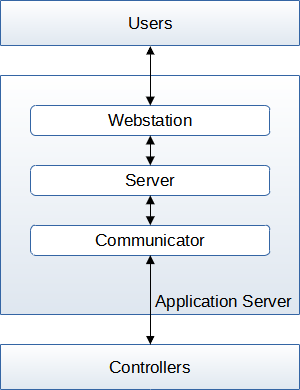
\includegraphics[width=0.3\textwidth]{images/scada_architecture.png}
    \caption{Arquitectura general de Rapid SCADA \cite{rapidscada_architecture}}
    \label{fig:scada_architecture}
\end{figure}

Els components principals de Rapid SCADA funcionen com a serveis del sistema operatiu, iniciant-se automàticament per garantir la disponibilitat contínua del sistema.

En entorns Linux, aquests serveis es gestionen mitjançant eines com \texttt{systemctl}, mentre que en Windows es poden administrar des de les eines pròpies del sistema o des de l'Administrator \cite{rapidscada_services}.

\subsection{Descripció dels components}

\subsubsection*{Webstation}


És l'aplicació web encarregada de la visualització de dades i la interacció amb l'usuari. Permet accedir al sistema SCADA mitjançant un navegador web sense necessitat d'instal·lar programari addicional

Permet representar informació en forma de taules, gràfics o sinòptics, així com consultar dades històriques i enviar comandes. L'accés està controlat mitjançant usuaris i permisos definits per l'administrador i existeix la possibilitat d'ampliar aquesta aplicació mitjançant plugins per adaptar-se a diferents necessitats de visualització \cite{rapidscada_apps}.


\subsubsection*{Communicator}

És el component responsable de la comunicació amb els dispositius de camp, com PLCs, sensors i controladors industrials.

La seva funció principal és adquirir dades en temps real i enviar comandes, gestionant múltiples línies de comunicació i diferents protocols industrials. Funciona en segon pla i registra l'activitat en fitxers de log per facilitar el diagnòstic d'errors \cite{rapidscada_apps}.

\subsubsection*{Server}

Aquest component és el nucli del sistema Rapid SCADA. S'encarrega de gestionar l'emmagatzematge de dades, el processament i la distribució de la informació a la resta d'aplicacions.

Gestiona tant les dades en temps real com les històriques, controla l'accés dels usuaris i proporciona la informació a la resta de components. Funciona com un servei en execució contínua, sense interfície d'usuari. La seva configuració es realitza des de l'aplicació Administrator. La seva funcionalitat es pot ampliar mitjançant mòduls addicionals \cite{rapidscada_apps}.


\subsubsection*{Agent}

L'\textit{Agent} és un servei encarregat de la gestió remota i la comunicació entre una instància de Rapid SCADA i l'aplicació Administrator.

Facilita la transferència de configuracions i l'accés als registres del sistema, permetent treballar tant en local com de forma remota mitjançant connexió TCP (port 10002 per defecte) \cite{rapidscada_apps}. Aquest component no disposa d'interfície gràfica i el seu funcionament es verifica mitjançant els registres del sistema.

\subsubsection*{Administrator}

Per últim, \textit{Administrator} és l'eina principal de desenvolupament i configuració de Rapid SCADA. Actua com un entorn integrat que permet definir tota l'estructura del sistema.

Facilita la transferència de configuracions i l'accés als registres del sistema, permetent treballar tant en local com de forma remota mitjançant connexió TCP \cite{rapidscada_apps}.


També incorpora eines que faciliten el desenvolupament:
\begin{itemize}
    \item Assistents (wizards) per crear dispositius i canals
    \item Importació i exportació de configuracions
    \item Clonació de canals
    \item Funcions de cerca, filtratge i ordenació
\end{itemize}



\subsection{Configuració amb ScadaAdmin}

La configuració del sistema SCADA s'ha realitzat mitjançant l'eina \textit{ScadaAdmin}, que actua com a entorn principal de desenvolupament \cite{rapidscada_config_basics}. Aquesta permet crear i desplegar projectes que defineixen completament el sistema mitjançant fitxers, principalment en format XML.

Un projecte de Rapid SCADA es divideix en diferents blocs principals:

\begin{itemize}
    \item \textbf{Configuration Database}: defineix l'estructura del sistema (objectes, dispositius, canals, usuaris)
    \item \textbf{Views}: conté les visualitzacions
    \item \textbf{Server, Communicator i Webstation}: configuració dels serveis del sistema
\end{itemize}

\subsubsection{Mòdul Database}

La base de dades de configuració és el nucli del sistema. Durant el desenvolupament es treballa en XML, però en el desplegament es transforma a format binari \texttt{.dat} optimitzat \cite{rapidscada_database}.


\subsubsection*{Primary Tables}

Les \textbf{taules primàries} defineixen el funcionament principal del sistema. Són les més importants i s'han de configurar amb cura.

\begin{itemize}
    \item \textbf{Objects}: estructura jeràrquica del sistema (planta, línies, màquines)
    \item \textbf{Communication Lines}: defineixen les línies de comunicació amb els dispositius
    \item \textbf{Devices}: llista de dispositius físics o virtuals
    \item \textbf{Channels}: canals de dades (variables del sistema, sensors, actuadors)
    \item \textbf{Limits}: límits de valors (alarmes)
    \item \textbf{Views}: configuració de les visualitzacions
    \item \textbf{Roles i Users}: gestió d'usuaris i permisos
\end{itemize}

Aquestes taules estan interrelacionades. Per exemple, un dispositiu està associat a una línia de comunicació, i un canal està associat a un dispositiu.

\subsubsection*{Secondary Tables}

Les \textbf{taules secundàries} complementen la configuració del sistema amb informació auxiliar.

\begin{itemize}
    \item \textbf{Archive kinds i Archives}: tipus i configuració d'arxius històrics
    \item \textbf{Channel types i Data types}: tipus de dades
    \item \textbf{Device types}: tipus de dispositius (drivers)
    \item \textbf{Formats}: formats de visualització
    \item \textbf{Units}: unitats de mesura
    \item \textbf{Scripts}: càlculs i fórmules
\end{itemize}

\subsubsection{Procés de configuració}

 El procés recomanat de configuració és el següent \cite{rapidscada_config_basics}:

\begin{enumerate}
    \item Crear un nou projecte
    \item Definir objectes, línies de comunicació i dispositius
    \item Configurar el Communicator i la comunicació amb els dispositius
    \item Crear canals per gestionar les dades
    \item Definir visualitzacions (Views)
    \item Desplegar el projecte al servidor
\end{enumerate}

Aquest procés s'ha seguit en el desenvolupament del present TFG, adaptant-lo a la simulació de la planta industrial implementada en Unity.

\subsection{Visualització i interfícies}
La visualització es basa en el concepte de \textbf{Views} \cite{rapidscada_views}, que permeten representar i interactuar amb les dades del sistema a través de la Webstation.


\subsubsection*{Tipus de vistes (\textit{Views})}

Rapid SCADA inclou per defecte diversos tipus de vistes, tot i que el sistema és extensible mitjançant plugins. Cada vista es correspon amb un fitxer dins del directori \textit{Views} del projecte. Els tipus principals de vistes són:


\begin{itemize}
    \item \textbf{Table View} → fitxers de visualització tabular
    \item \textbf{Mimic Diagram} → esquemes gràfics del procés 
    \item \textbf{SchemClassic} → esquemes clàssics 
    \item \textbf{Faceplate} → components reutilitzables 
    \item \textbf{XML File} → configuracions personalitzades
    \item \textbf{Text File} → suport per definicions manuals
\end{itemize}


\subsubsection*{Execució de les vistes}

Les vistes es mostren a través de la \textbf{Webstation}, que és l'aplicació web de Rapid SCADA accessible des d'un navegador. El procés de visualització és el següent:

\begin{enumerate}
    \item Configuració a ScadaAdmin
    \item Registre a la taula Views
    \item Desplegament del projecte
    \item Accés des de Webstation segons permisos
\end{enumerate}

Les vistes poden incloure paràmetres com objecte associat, ordre o configuració específica (Figura \ref{fig:rapidscada_views}).

En el cas de les \textbf{Table Views}, aquestes permeten visualitzar dades històriques i en temps real. A més a més, es poden generar gràfiques clicant sobre els valors, permeten enviar comandes als dispositius i  utilitzen arxius històrics (Min, Hour, etc.) com a font de dades

La funcionalitat de les vistes es pot ampliar mitjançant plugins, que permeten crear interfícies més avançades i adaptades a les necessitats del sistema, com es detallarà en apartats posteriors.



\begin{figure}[H]
    \centering
    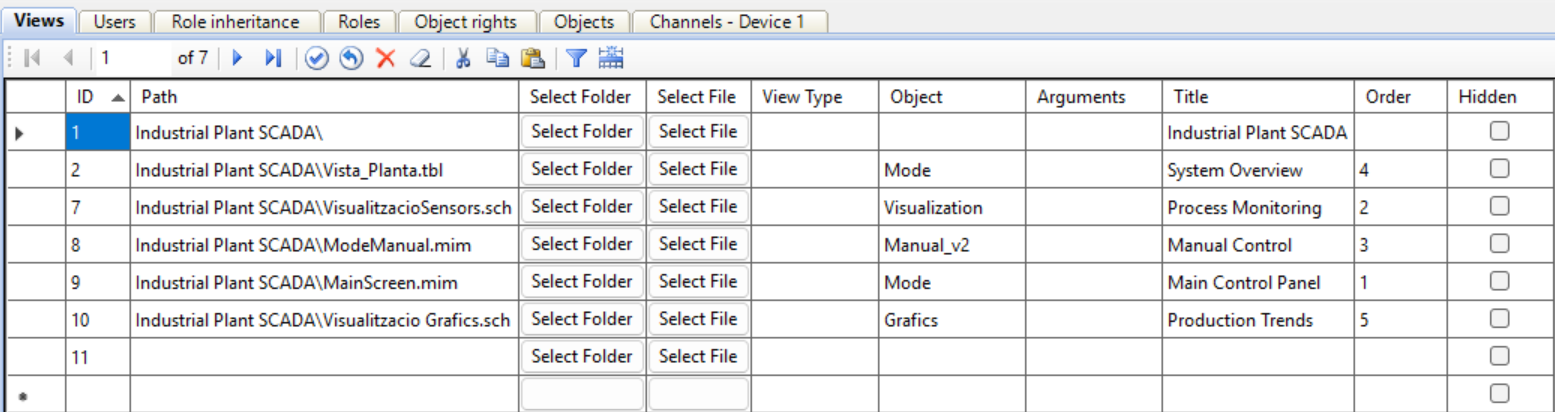
\includegraphics[width=0.7\textwidth]{images/views_scada.png}
    \caption{Taula \textit{Views} de RapidScada}
    \label{fig:rapidscada_views}
\end{figure}

\vspace{2cm}
\subsection{Comunicacions i dispositius}

\begin{wrapfigure}[17]{r}{0.38\textwidth}
    \centering
    \vspace{0pt}
    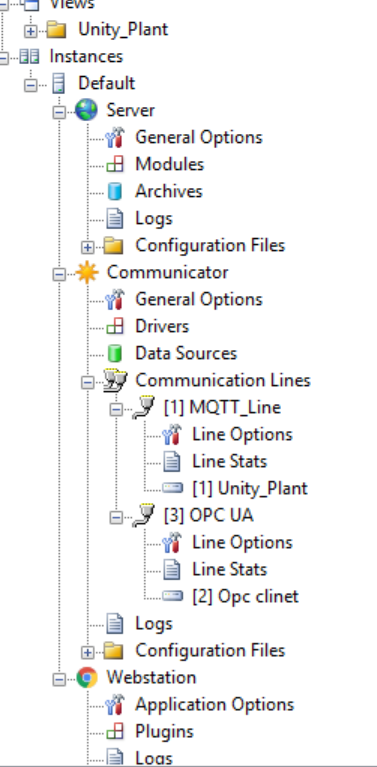
\includegraphics[width=0.33\textwidth]{images/communication.png}
    \caption{Jerarquia de RapidScada}
    \label{fig:rapidscada_comm}
\end{wrapfigure}

La comunicació amb dispositius es gestiona mitjançant el mòdul \textbf{Communicator} i es basa en tres elements: \textbf{Communication Lines}, \textbf{Devices} i \textbf{Channels} \cite{rapidscada_device_polling, rapidscada_channels}. Aquest elements es troben relacionats entre si, és a dir, una línia de comunicació conté diversors dispositius, i cada dispositiu pot està associat a múltiples canals. La configuració s'ha de realitzar seguint una seqüència lògica per garantir la coherència del sistema (Figura \ref{fig:rapidscada_comm}).


\subsubsection*{Communication Lines}

Les línies de comunicació defineixen el mètode de connexió i permeten gestionar diverses connexions simultàniament.
Entre els principals tipus de línies suportades es troben: \textit{Port sèrie}, \textit{TCP Client}, \textit{TCP Server}, \textit{UDP} i \textit{MQTT Client}.


\subsubsection*{Devices i polling}


Els \textbf{dispositius} representen els dispositius físics o fonts de dades del sistema (PLC, sensors, actuadors o simuladors) \cite{rapidscada_device_polling}. Cada dispositiu s'assigna a una \textit{Communication Line}, que defineix el canal de comunicació general, però la configuració específica del protocol es realitza principalment en el dispositiu mitjançant el \textbf{driver} seleccionat.

És a dir, la \textit{Communication Line} estableix el tipus de connexió (TCP, sèrie, MQTT, etc.), mentre que el \textit{Device} defineix com es comunica realment amb aquell equip. En alguns casos, com amb OPC UA o MQTT, la configuració pot dependre gairebé exclusivament del dispositiu.

En crear un dispositiu, es defineix el seu \textbf{device type} (driver), i posteriorment es poden ajustar els paràmetres principals dins de les opcions del dispositiu:


\begin{itemize}
    \item Driver (protocol de comunicació) i adreça (del dispositiu real amb el que vols comunicar-te.)
    \item Timeout i Delay
    \item Estat d'activació
\end{itemize}

El paràmetre \textbf{polling} determina en quin format específic es llegeixen les dades del dispositiu (cíclic, periòdic o sota demanda).

\subsubsection*{Channels}

Els canals són les unitats bàsiques de dades dins del SCADA (equivalents a variables o tags). Cada canal està associat a un dispositiu i a una variable concreta (sensor, estat, actuador, ...).

Les propietats més rellevants són:

\begin{itemize}
    \item \textbf{Data type}: tipus de dada (numèrica, booleana, etc.)
    \item \textbf{Tag}: identificador vinculat amb el dispositiu
    \item \textbf{Format}: representació visual
    \item \textbf{Limits}: definició d'alarmes
    \item \textbf{Archives}: on es guarden les dades (Min, Hour, etc.)
\end{itemize}

Els canals permeten registrar dades històriques, generar esdeveniments i enviar comandes als dispositius

\subsection{Gestió de perfils de seguretat}
\label{sec:scada_users}

%%\subsubsection{Model de control d'accés}

Rapid SCADA utilitza un model de control d'accés basat en tres elements principals: \textbf{objectes}, \textbf{rols} i \textbf{usuaris} \cite{rapidscada_user_management}.

En primer lloc, es defineixen els \textbf{objectes}, que representen les diferents parts del sistema (planta, dispositius, zones o funcionalitats). Aquests objectes es poden organitzar de forma jeràrquica, permetent estructurar el sistema de manera lògica.

A continuació, es creen els \textbf{rols}, que defineixen un conjunt de permisos. A cada rol se li assignen drets específics sobre cada objecte, com ara visualització de dades o enviament de comandes.

Finalment, els \textbf{usuaris} es vinculen a un rol determinat. D'aquesta manera, cada usuari hereta automàticament els permisos associats al rol assignat. Aquest model permet una gestió flexible i escalable dels accessos dins del sistema.

\subsubsection*{Creació d'usuaris i assignació de rols}

Els usuaris es defineixen a la taula \textit{Users} i s'associen a un rol.

Alguns usuaris i rols bàsics es creen per defecte, com ara:
\begin{itemize}
    \item \textbf{Administrator}: accés complet
    \item \textbf{Dispatcher}: visualització i control
    \item \textbf{Guest}: només visualització
\end{itemize}

També es poden crear rols personalitzats amb permisos configurables, simplificant la gestió en sistemes complexos.


\subsubsection*{Permisos i control d'accés}

Els permisos es defineixen a la taula \textit{Object rights}, indicant què pot fer cada rol sobre cada objecte.

Aquest sistema permet controlar accions com:
\begin{itemize}
    \item Visualitzar dades
    \item Accedir a pantalles
    \item Enviar comandes
\end{itemize}

Només els rols personalitzats poden tenir permisos configurables, ja que els rols predefinits ja tenen els seus drets definits internament. La informacó respecte els permisos que té cada rol es pot trobar a la \textit{Rights Matrix} (Figura \ref{fig:rights_matrix}), on la lletra \textit{V} significa \textit{View} (visualització de la pantalla) i la lletra \textit{C} significa \textit{Control} (interactuar amb la pantalla). 

\begin{figure}[H]
    \centering
    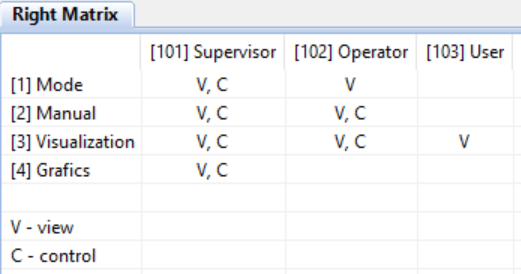
\includegraphics[width=0.5\textwidth]{images/right_matrix.png}
    \caption{Exemple de Rights Matrix a Rapid SCADA}
    \label{fig:rights_matrix}

\end{figure}

A més a més, Rapid SCADA permet definir \textbf{herència de rols}, de manera que un rol pot heretar els permisos d'ltres rols. Això permet reutilitzar configuracions i reduir la complexitat. A part, com que els objectes poden estar organitzats jeràrquicament, els permisos assignats a un objecte superior es propaguen als seus subobjectes, facilitant la gestió en sistemes grans.


\subsection{Gestió de dades i emmagatzematge}

Rapid SCADA incorpora diferents mecanismes per gestionar i emmagatzemar la informació generada pel sistema. Les dades provinents dels dispositius i canals són processades pel mòdul \textit{Server}, que s'encarrega tant de la gestió en temps real com de l'emmagatzematge històric \cite{rapidscada_apps}.

Per defecte, el sistema utilitza un mecanisme d'emmagatzematge intern basat en fitxers binaris amb extensió \texttt{.dat}, ubicats principalment a la carpeta \textit{Archive}. Aquest format està optimitzat per al registre continu de dades industrials i permet un accés eficient a grans volums d'informació temporal.

Les dades històriques poden ser consultades des de la mateixa \textit{Webstation} mitjançant taules, gràfiques i tendències, sense necessitat d'accedir directament als fitxers interns del sistema. Aquest enfocament prioritza el rendiment i la fiabilitat del sistema per sobre de l'accés extern directe a les dades.

A més de l'emmagatzematge intern, Rapid SCADA permet integrar bases de dades externes com \textbf{PostgreSQL} o \textbf{InfluxDB} mitjançant mòduls i plugins específics \cite{rapidscada_db_export}. Aquesta funcionalitat facilita:

\begin{itemize}
    \item L'emmagatzematge de dades en formats consultables externament
    \item La realització d'anàlisi avançada i informes personalitzats
    \item La integració amb altres aplicacions industrials o plataformes IIoT
\end{itemize}

En aquests casos, les dades generades pel sistema SCADA es transfereixen des del sistema intern cap a la base de dades externa, permetent l'execució de consultes SQL o l'anàlisi de sèries temporals segons la tecnologia utilitzada.


\subsection{Plugins de Rapid SCADA}

%%\subsubsection{Consideracions generals sobre plugins}

Rapid SCADA permet ampliar les seves funcionalitats mitjançant \textbf{plugins} i mòduls addicionals. En el cas de la Webstation, aquests mòduls s'anomenen plugins i permeten estendre la interfície d'usuari i les capacitats de visualització. Mitjançant plugins es poden implementar:
\begin{itemize}
    \item Nous tipus de vistes
    \item Components gràfics per a esquemes
    \item Gràfiques i informes avançats
\end{itemize}

Es desenvolupen en \textit{.NET} \cite{rapidscada_dev_basics} i s'integren com a llibreries \texttt{.dll}. També es poden obtenir des del repositori oficial o des de la botiga de mòduls de Rapid SCADA.

\subsubsection{Sistema de llicències i instal·lació}

Els plugins poden tenir diferents modalitats:
\begin{itemize}
    \item \textbf{Gratuïts}: inclosos per defecte o disponibles públicament
    \item \textbf{De pagament}: requereixen registre i clau de llicència
    \item \textbf{Versió \textit{trial}}: funcionament limitat sense registre, el qual ens obliga a demanar un codi que dura 24 hores cada vegada que volguem instal·lar aquests plugins. 
\end{itemize}

El procés d'instal·lació consisteix en:
\begin{itemize}
    \item Copiar els fitxers del plugin a la carpeta d'instal·lació de SCADA
    \item Activar-lo des de \textit{ScadaAdmin}.
    \item Configurar-lo segons la seva documentació
    \item Carregar el projecte al sistema
\end{itemize}


\subsubsection{Plugins utilitzats en el projecte}

\subsubsection*{Chart Pro Plugin}

Aquest plugin \cite{rapidscada_chart_pro} amplia les capacitats de visualització de dades, permetent representar gràfiques avançades amb múltiples canals simultanis.

Les seves funcionalitats principals són:
\begin{itemize}
    \item Visualització de múltiples canals en un mateix gràfic
    \item Modes de visualització (fix o dinàmic)
    \item Exportació a formats com PNG o PDF
    \item Configuració mitjançant perfils
\end{itemize}

S'ha utilitzat per representar l'evolució temporal de variables del sistema, millorant la visualització respecte al sistema base (Figura \ref{fig:chart_pro}).


\begin{figure}[H]
    \centering
    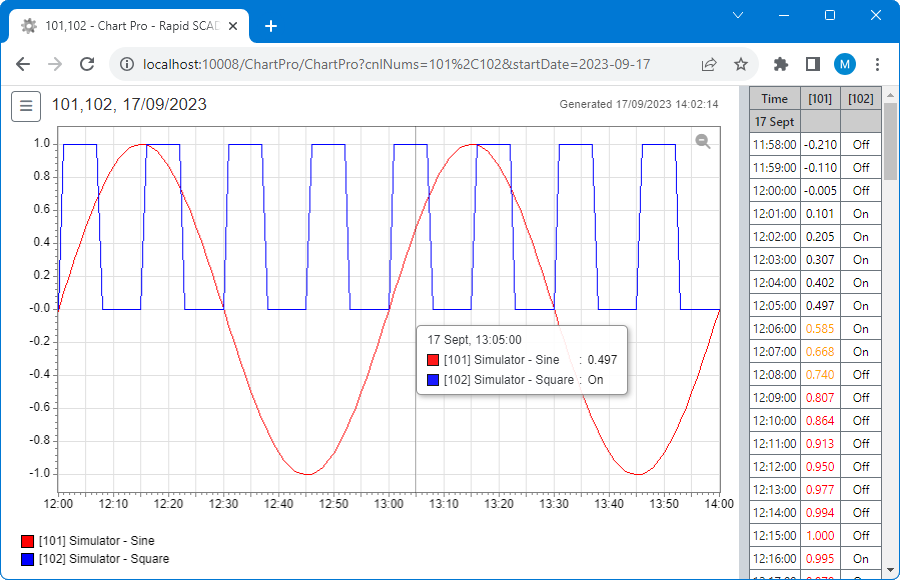
\includegraphics[width=0.5\textwidth]{images/chart-pro-exemple.png}
    \caption{Exemple del modul ChartPro \cite{rapidscada_chart_pro}}
    \label{fig:chart_pro}
\end{figure}

\subsubsection*{Extra Scheme Editor}

El sistema base de Rapid SCADA permet la creació d'esquemes mitjançant fitxers \texttt{.sch}, amb elements bàsics com textos, imatges, botons, indicadors (LED) i enllaços (Aplicació d'aquesta part en l'apartat \ref{sec:hmi}). El \textbf{Extra Scheme Editor} amplia aquestes funcionalitats afegint nous components gràfics com \textbf{Chart} (gràfiques de dades), \textbf{Trend}, \textbf{Gauge} (indicadors analògics) o \textbf{Frame}

Especialment rellevant és l'ús del component \textbf{Chart}, que, combinat amb el Chart Pro Plugin, permet visualitzar múltiples canals en temps real dins dels esquemes.

Tot i això, cal destacar que les gràfiques integrades en fitxers \texttt{.sch} tenen funcionalitats més limitades en comparació amb les visualitzacions generades des de les vistes de tipus taula (\texttt{.tbl}). En aquestes últimes, en seleccionar una variable amb dades històriques, es poden generar gràfiques més completes, amb opcions avançades com la selecció de períodes de temps o la visualització detallada de l'evolució de les dades.

\subsubsection*{Mimic Editor}

El \textbf{Mimic Editor} és un plugin que permet crear interfícies gràfiques més avançades i flexibles que els fitxers \texttt{.sch}.

A diferència dels esquemes tradicionals, aquest editor permet:
\begin{itemize}
    \item Associar comportaments dinàmics als elements gràfics 
    \item Definir accions en interaccions (clics) (no solament als botons o al \textit{toggle}).
    \item Enviar valors específics directament a canals (control actiu) sense limitació
\end{itemize}

A més, permet integrar els components del \textit{Extra Scheme Editor}, combinant visualització i control en una mateixa interfície.

Aquest plugin ha estat clau en el desenvolupament del projecte, ja que permet una interacció més completa amb el sistema SCADA i facilita la implementació del control sobre la planta simulada.

\newpage
\section{Fonaments teòrics de Unity}
\label{sec:unity_theory}
\subsection{Introducció a Unity}

%%\subsubsection{Què és Unity i per a què serveix}

La plataforma Unity (també coneguda com \textit{Unity3D}, figura \ref{fig:logo_unity}) és un motor de desenvolupament en temps real utilitzat principalment per a la creació d'aplicacions interactives en 2D i 3D, especialment en l'àmbit dels videojocs. Aquest motor permet als desenvolupadors dissenyar, simular i executar entorns virtuals mitjançant una combinació d'un editor visual i un sistema de programació basat en \textit{scripts} \cite{Unity}.

A diferència d'altres eines més específiques, Unity es caracteritza per ser una plataforma multiplataforma, la qual permet desenvolupar una aplicació una sola vegada i exportar-la a diferents sistemes com ordinadors, dispositius mòbils, consoles o entorns web.

A nivell funcional, Unity proporciona eines per gestionar gràfics, física, il·luminació, animacions i interacció amb l'usuari, tot integrat dins d'un mateix entorn de desenvolupament \cite{UnityOfficial, UnityDocsManual}. Això facilita el procés de creació de projectes complexos sense necessitat de desenvolupar un motor des de zero.

\begin{figure}[H]
    \centering
    
\includegraphics[width=0.35\linewidth]{images/logo_unity.png}
    \caption{Logotip oficial del motor Unity}
    \label{fig:logo_unity}
\end{figure}

\subsubsection{Contextos d'aplicació de Unity}

Tot i que Unity va ser concebut inicialment com un motor per al desenvolupament de videojocs \cite{UnityWikipedia}, amb el pas del temps s'ha convertit en una eina utilitzada en múltiples àmbits gràcies a la seva flexibilitat i capacitat de simulació en temps real \cite{UnityLearnIntro}.  Actualment, Unity s'utilitza en sectors com:

\begin{itemize}
\item \textbf{Videojocs:} és un dels motors més utilitzats per desenvolupadors independents i estudis professionals.
\item \textbf{Simulació industrial:} permet crear bessons digitals i entorns virtuals per simular processos reals.
\item \textbf{Realitat virtual (VR) i realitat augmentada (AR):} facilita el desenvolupament d'experiències immersives.
\item \textbf{Arquitectura i enginyeria:} per visualitzar projectes en 3D abans de la seva construcció.
\item \textbf{Educació i recerca:} s'utilitza per crear entorns interactius i simulacions experimentals.
\end{itemize}

Aquesta versatilitat es deu al fet que Unity ha evolucionat d'un simple motor de videojocs a una plataforma general de creació de contingut interactiu en temps real.



\subsubsection{Evolució del motor Unity al llarg dels anys}

Unity va ser desenvolupat per l'empresa Unity Technologies i presentat per primera vegada l'any 2005. Inicialment, el seu objectiu era proporcionar un motor assequible per a desenvolupadors independents, que fins aquell moment tenien dificultats per accedir a tecnologies similars.

Amb el temps, Unity ha anat evolucionant tant en funcionalitats com en àmbits d'aplicació \cite{UnityLearnIntro}. En els seus inicis estava centrat exclusivament en el desenvolupament de videojocs, però progressivament ha incorporat millores en el renderitzat, la física, la compatibilitat multiplataforma i la integració amb noves tecnologies com la realitat virtual o la intel·ligència artificial.

Un dels aspectes més rellevants de la seva evolució és que ha facilitat molt el desenvolupament d'aplicacions, permetent que persones o petits equips puguin crear projectes complexos sense necessitat de disposar de grans recursos ni de desenvolupar eines pròpies des de zero.

Actualment, Unity és considerat un dels motors de desenvolupament més utilitzats a nivell mundial, amb una gran comunitat d'usuaris i una àmplia documentació disponible \cite{UnityWikipedia}.

\subsection{Característiques generals del motor}

\subsubsection{Treball en entorns 2D i 3D}

Unity permet desenvolupar aplicacions tant en 2D com en 3D dins d'un mateix entorn de treball. Per un costat, en entorns 2D, proporciona eines específiques com el sistema de \textit{Sprites}, física 2D independent i càmeres ortogràfiques, facilitant el desenvolupament d'aplicacions basades en gràfics plans.

Per l'altre costat, en entorns 3D, incorpora un sistema complet de representació espacial amb càmeres en perspectiva, il·luminació avançada i simulació física tridimensional, permetent desenvolupar entorns immersius com el sistema virtual d'aquest projecte \cite{Unity2Dor3D}.

\subsubsection{Capacitats de renderització}
Com a factor interessant, consta d'un sistema de renderització en temps real basat en la GPU, que permet visualitzar escenes de forma eficient \cite{GPUWikipedia}. Ofereix diferents \textit{Render Pipelines} \cite{UnityRenderPipelines}, entre els quals destaquen:
\begin{itemize}
    \item \textbf{Built-in Render Pipeline}: sistema clàssic amb configuració senzilla però menys flexible.
    \item \textbf{Universal Render Pipeline (URP)}: utilitzat en aquest projecte per oferir un bon equilibri entre rendiment i qualitat.
    \item \textbf{High Definition Render Pipeline (HDRP)}: orientat a visualitzacions d'alt realisme.
\end{itemize}

Aquesta flexibilitat permet adaptar el motor a diferents necessitats, des de simulacions senzilles fins a entorns visuals complexos.

\subsubsection{Tipus de projectes que es poden desenvolupar}

Unity permet crear diferents tipus de projectes segons la configuració inicial seleccionada dins del \textit{Unity Hub} (figura \ref{fig:menu_unity}). Entre els principals tipus destaquen \cite{UnityProjectTemplates}:

\begin{itemize}
    \item \textbf{Projectes 2D}: orientats a videojocs o aplicacions amb gràfics plans.
    \item \textbf{Projectes 3D (URP)}: utilitzats en la majoria d'aplicacions, incloent simulacions industrials com la desenvolupada en aquest treball.
    \item \textbf{Projectes HDRP}: enfocats a visualitzacions d'alt realisme (arquitectura, simulació avançada).
    \item \textbf{Realitat Virtual (VR)}: per al desenvolupament d'entorns immersius amb dispositius com ulleres VR.
    \item \textbf{Realitat Augmentada (AR)}: aplicacions que combinen elements virtuals amb el món real.
    \item \textbf{Mixed Reality (MR)}: combinació avançada de VR i AR.
\end{itemize}


\begin{figure}[H]
    \centering
    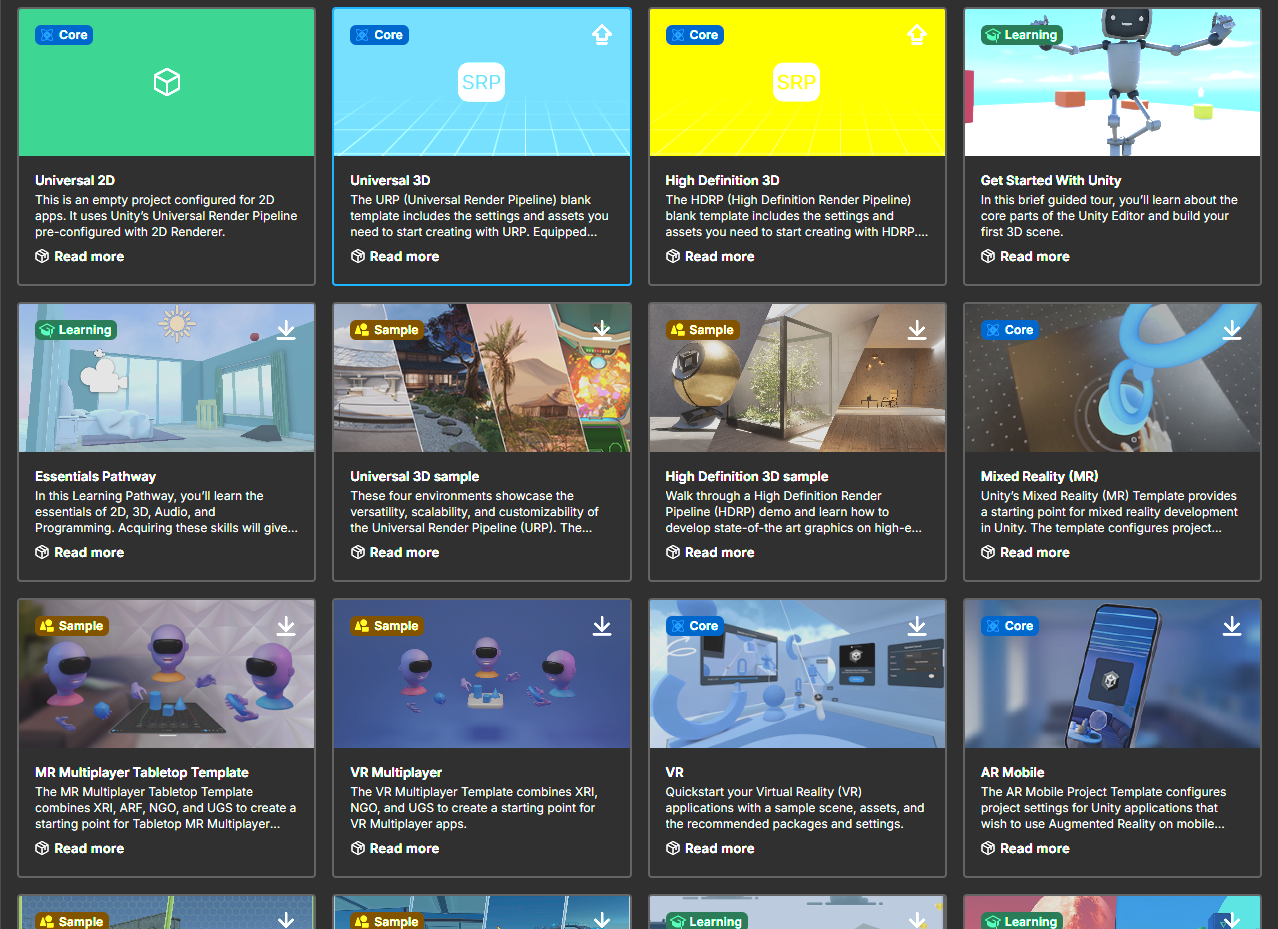
\includegraphics[width=0.4\linewidth]{images/menu_unity_1.png}
    \caption{Menu de projectes}
    \label{fig:menu_unity}
\end{figure}

\subsubsection{Procés de creació d'un projecte}

La creació d'un projecte a Unity segueix una sèrie de fases que permeten desenvolupar aplicacions de manera estructurada i modular. Inicialment, des del \textit{Unity Hub} es crea un nou projecte seleccionant la plantilla més adequada segons el tipus d'aplicació que es vol desenvolupar \cite{UnityCreateProject}.

Una vegada creat el projecte, el desenvolupament es basa principalment en la construcció d'escenes (\textit{Scenes}), que representen els diferents espais o entorns de treball dins de l'aplicació \cite{UnityScenes}. A partir d'aquí, el procés habitual de desenvolupament inclou les següents etapes:

\begin{itemize}
    \item Creació de l'escena i col·locació dels objectes
    \item Importació de models 3D, materials i textures
    \item Configuració de components i propietats físiques
    \item Programació del comportament mitjançant scripts en C\#
    \item Execució, simulació i proves del sistema
\end{itemize}

Aquest procés de treball permet desenvolupar aplicacions de forma iterativa, facilitant la modificació i ampliació del projecte durant totes les fases del desenvolupament. En aquest treball, aquesta metodologia ha permès construir la simulació de la planta industrial de manera modular i escalable.
\subsection{Entorn de desenvolupament de Unity}

%%\subsubsection{Estructura general de l'editor}

L'editor de \textit{Unity} \cite{UnityEditorInterface} està format per diferents finestres que permeten gestionar tots els elements d'un projecte de manera visual i interactiva. Aquest entorn es pot personalitzar segons les necessitats de l'usuari, però per defecte presenta una distribució estàndard amb les principals eines de desenvolupament. En la figura \ref{fig:MenuEditor} es mostren les finestres més rellevants de l'editor, que són essencials per a la creació i gestió de projectes a Unity.

\begin{figure}[H]
    \centering
    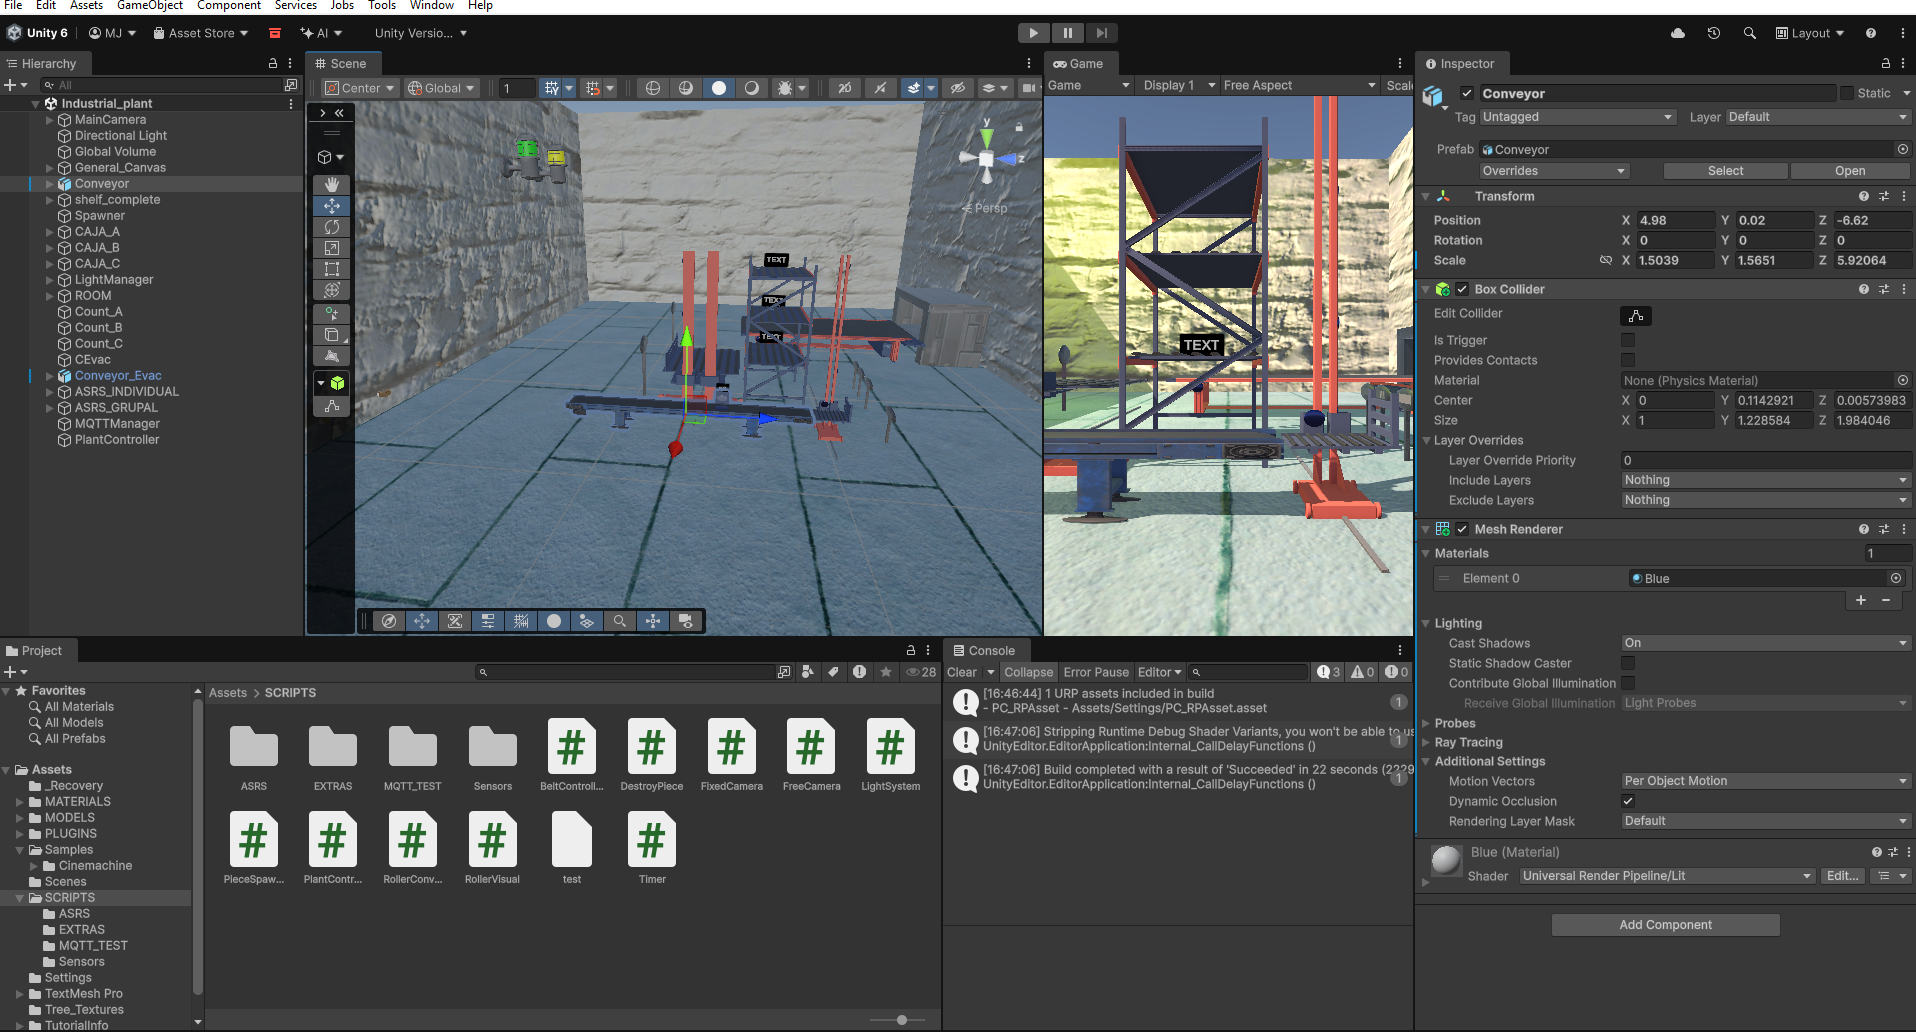
\includegraphics[width=0.95\linewidth]{images/menu_editor.png}
    \caption{Distribució estàndard de l'editor de Unity}
    \label{fig:MenuEditor}
\end{figure}


\subsubsection{Vistes i jerarquia}

A les finestres centrals es situen les dues vistes la d'escena i la de joc, juntament amb els objectes que permeten muntar una escena. 

A la vista \textit{Scene} \cite{UnityScenes} s'observa l'espai on es construeix el món virtual. Permet visualitzar i manipular els objectes en un entorn 2D o 3D, modificar la seva posició, rotació i escala, així com organitzar-los dins de l'escena. Aquesta vista és \textbf{interactiva} i no representa el resultat final del joc, sinó una eina de disseny.

A la vista \textit{Game} es mostra la representació final del joc tal com la veuria l'usuari. Aquesta vista depèn de les càmeres de l'escena i permet executar el projecte en temps real mitjançant el botó de \textit{Play}.

En l'\textit{Inspector} \cite{UnityInspector} es pot visualitzar i modificar totes les propietats dels objectes seleccionats. Quan es selecciona un objecte, l'Inspector mostra tots els seus components (transformacions, materials, scripts, etc.) i permet editar-los (figura \ref{fig:menu_editor_inspector}).

\begin{figure}[H]
    \centering
    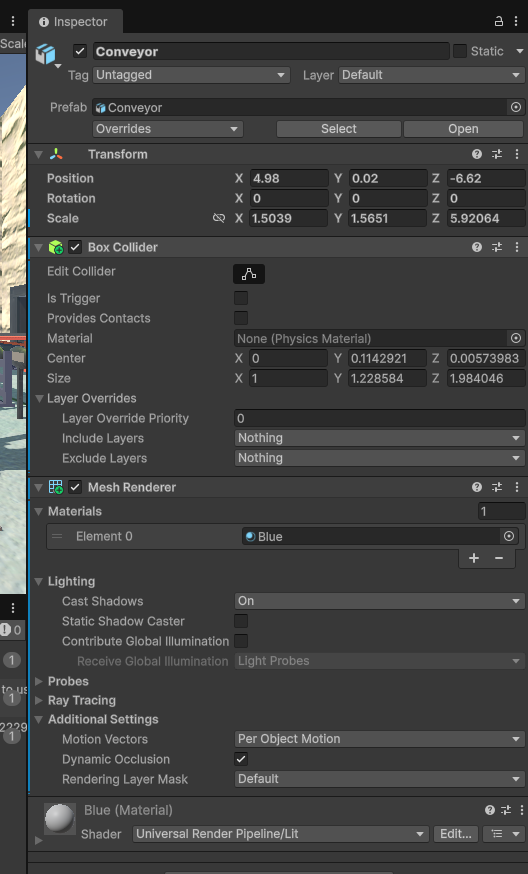
\includegraphics[width=0.3\linewidth]{images/menu_editor_insp.png}
    \caption{Finestra Inspector de Unity amb característiques d'un objecte seleccionat}
    \label{fig:menu_editor_inspector}
\end{figure}

A la finestra \textit{Hierarchy} \cite{UnityHierarchy} es mostra tots els objectes (\textit{GameObjects}) presents en l'escena actual, organitzats en forma d'arbre jeràrquic.

\begin{figure}[H]
    \centering
    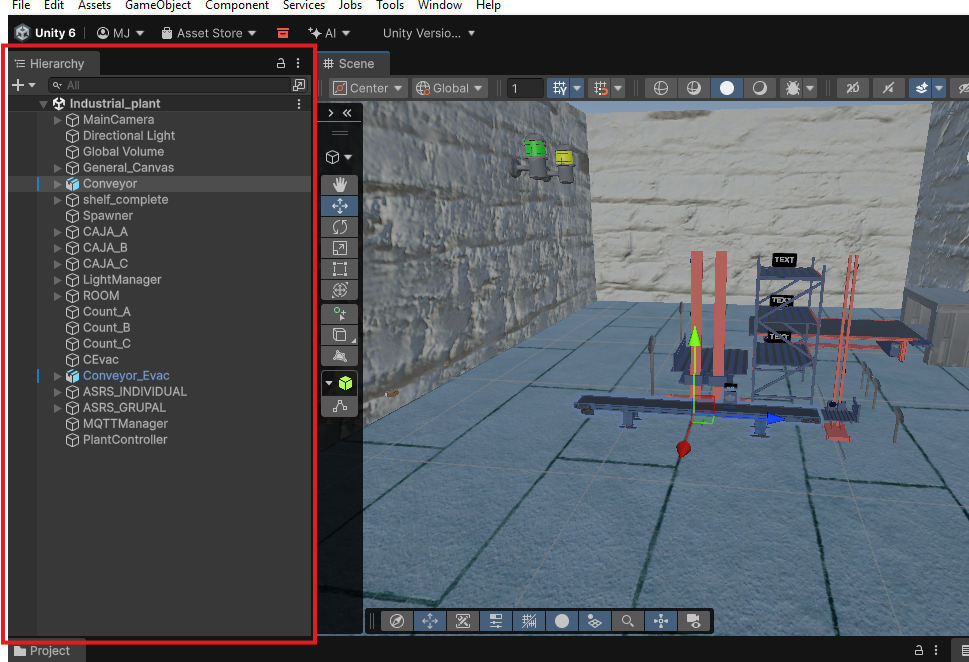
\includegraphics[width=0.6\linewidth]{images/menu_editor_hier.png}
    \caption{Finestra Hierarchy que mostra l'estructura jeràrquica dels GameObjects}
\end{figure}

Aquesta estructura permet establir relacions pare-fill entre objectes, facilitant la seva organització i manipulació. 


\subsubsection*{Gestió de components}

Cada objecte a Unity està format per components \cite{UnityComponents}. Aquests defineixen el seu comportament i característiques (per exemple, \textit{Transform}, \textit{Renderer}, \textit{Collider} o scripts personalitzats). Des de l'Inspector es poden afegir nous components mitjançant el botó \textit{Add Component}, així com modificar les seves propietats.

\subsubsection*{Tags i Layers}

Unity permet assignar \textit{Tags} i \textit{Layers} als objectes per facilitar la seva identificació i gestió \cite{UnityTags2023}.

\begin{itemize}
    \item \textbf{Tags}: permeten identificar objectes (per exemple, "Player" o "Box").
    \item \textbf{Layers}: s'utilitzen principalment per controlar col·lisions i càmeres.
\end{itemize}


\subsubsection*{Gestió de paquets (Package Manager)}

El \textit{Package Manager} \cite{UnityPackageManager} és una eina integrada en Unity que permet afegir i gestionar funcionalitats addicionals mitjançant paquets, els quals inclouen recursos, scripts i eines que amplien les capacitats del motor. Aquesta eina facilita la instal·lació i actualització de components dins del projecte des d'una única interfície (figura \ref{fig:package_manager}). 
En aquest projecte s'han utilitzat alguns paquets rellevants \cite{UnityPackagesDocs}:

\begin{itemize}

\item \textbf{Cinemachine}: Permet gestionar càmeres de forma avançada. Tot i que inicialment es va considerar per al control de càmera, finalment s'han reutilitzat alguns recursos visuals del paquet \cite{UnityCinemachine}.

\item \textbf{FBX Exporter}: Utilitzat per exportar models en format \textit{.fbx} i editar-los en eines externes (\textit{Blender}).

\item \textbf{Input System}: Sistema d'entrada de dades més flexible que permet gestionar diferents dispositius.

\item \textbf{ProBuilder}: Eina de modelatge integrada utilitzada per crear geometria directament dins de Unity.

\end{itemize}

\begin{figure}[h]
    \centering
    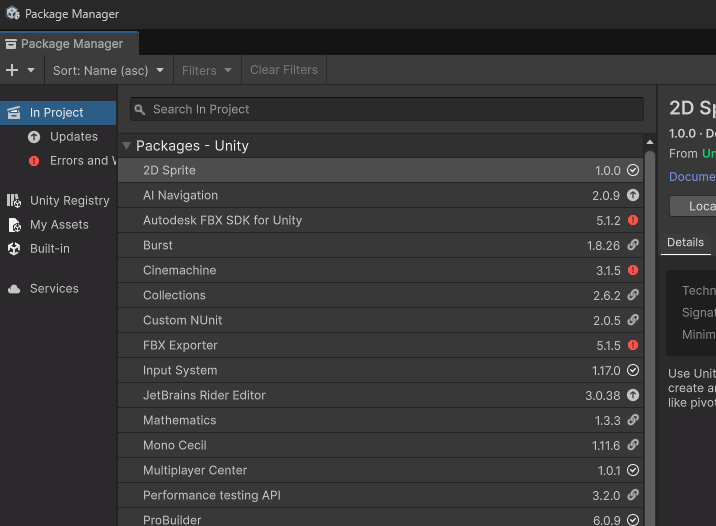
\includegraphics[width=0.5\linewidth]{images/unity_package_manager.png}
    \caption{Interfície del Package Manager de Unity}
    \label{fig:package_manager}
\end{figure}



\subsubsection{Eines i gestió de projectes}

Com a eina que pot ajudar a tindre un control del projecte, tenim que la consola (\textit{Console}) és l'eina que mostra missatges del sistema, errors i advertències generades durant l'execució del programa. És essencial per detectar errors en scripts i depurar el funcionament del sistema.

A més a més, observem que la barra superior de Unity conté els principals menús de gestió del projecte i accés a funcionalitats avançades del motor (figura \ref{fig:barra_superior}). 

\begin{figure}[H]
    \centering
    
\includegraphics[width=0.6\linewidth]{images/barra_superior.png}
    \caption{Barra superior del menú editor en Unity}
    \label{fig:barra_superior}
\end{figure}

\begin{itemize}
\item \textbf{File}: permet crear, obrir i guardar projectes i escenes.
\item \textbf{Edit}: inclou opcions de configuració, preferències i eines d'edició generals.
\item \textbf{Assets}: gestiona els recursos del projecte, permetent importar, exportar i organitzar fitxers.
\item \textbf{GameObject}: permet crear nous objectes dins de l'escena, com càmeres, llums o objectes buits.
\item \textbf{Component}: s'utilitza per afegir components als objectes seleccionats, definint el seu comportament.
\item \textbf{Services}: dona accés a serveis externs de Unity com analítica, multiplayer o monetització.
\item \textbf{Jobs}: relacionat amb el sistema de processament paral·lel de Unity per optimitzar el rendiment.
\item \textbf{Tools}: inclou eines addicionals, tant pròpies com instal·lades mitjançant paquets.
\item \textbf{Window}: permet obrir i gestionar les diferents finestres de l'editor, incloent el \textit{Package Manager}.
\item \textbf{Help}: proporciona accés a la documentació oficial, tutorials i suport.

\end{itemize}

\subsection{Gestió de materials i textures}

%%\subsubsection{Idees bàsiques respecte als materials}

En Unity, un \textit{material} defineix l'aspecte visual d'un objecte dins de l'escena, incloent propietats com el color, la brillantor o la resposta a la llum \cite{UnityMaterialsIntro}. 

Els materials es creen des del panell de \textit{Project} i es configuren a l'\textit{Inspector}. Cada material està associat a un \textbf{Shader}, que determina com es representa visualment l'objecte \cite{UnityShaders}.

Pel que fa a l'assignació d'aquests, els materials s'assignen als objectes mitjançant el component \textit{Mesh Renderer}, encarregat de la seva representació visual. Aquesta assignació es pot fer directament des de l'\textit{Inspector} o arrossegant el material sobre l'objecte. Un mateix material pot ser compartit entre diversos objectes \cite{UnityMaterialsReference}. 


\subsubsection{Importació de textures externes}

Les textures són imatges que aporten detall visual als materials, com el color o el relleu \cite{UnityMaterialsIntro}. En aquest projecte s'han utilitzat textures PBR (\textit{Physically Based Rendering}) provinents de repositoris externs, que permeten aconseguir resultats més realistes. El procés bàsic d'ús és:

\begin{enumerate}

\item \textbf{Importació de les textures}: Les textures s'afegeixen al projecte arrossegant-les a la carpeta \textit{Assets}. \cite{UnityImportTextures}
\item \textbf{Creació del material}: Es crea un material que actuarà com a contenidor de les textures.
\item \textbf{Assignació de mapes PBR}: Les textures s'assignen als canals corresponents del material, com el color base o el relleu (normal map), per definir el seu comportament visual.

\begin{itemize}

\item \textbf{Albedo (Base Map)}: color base del material.
\item \textbf{Normal Map}: detall superficial (relleu).  
\item \textbf{Metallic Map}:parts metàl·liques del material (actuació davant la llums)
\item \textbf{Height Map}: profunditat o desplaçament en la superfície del material.
\item \textbf{Ambient Occlusion (AO)}: ombres suaus on la llum arriba més difícilment

\end{itemize}


\item \textbf{Configuració del tipus de textura}: Algunes textures requereixen ajustos específics a l'\textit{Inspector}, com el cas dels \textit{Normal Maps}. \cite{UnityImportTextures}


\item \textbf{Ajust de propietats del material}: Després una vegada tens tots els elements seleccionats, sempre existeix la opció de modificar aquestes textures segons sembli més correcte a cadascú.

\end{enumerate}

\subsubsection{Propietats dels materials }

Els materials disposen de diverses propietats bàsiques:

\begin{itemize}

\item \textbf{Shader}: defineix com el material interactua amb la llum. \cite{UnityShaders}
\item \textbf{Color}: estableix el color base del material.
\item \textbf{Offset}: permet desplaçar la textura dins de l'objecte. \cite{UnityTextureProperties}

\end{itemize}

Aquestes propietats permeten ajustar i reutilitzar materials de forma eficient dins de l'escena. Addicionalment, Unity utilitza tècniques com el \textit{Physically Based Rendering (PBR)} per aconseguir resultats realistes sota diferents condicions d'il·luminació \cite{UnityMaterialsIntro}. 

\subsection{Sistema de components en Unity}

%%\subsubsection{Concepte de GameObject}

En Unity, qualsevol element present dins d'una escena es representa mitjançant un \textit{GameObject}, que constitueix la unitat bàsica de treball del motor gràfic \cite{UnityGameObjects}. Aquest component pot representar objectes visibles (peces, cintes, càmeres, ...), però també elements lògics (controladors, punts de referència...). 

Unity utilitza un model modular basat en composició, on cada funcionalitat s'implementa mitjançant components independents. Per exemple, un objecte pot incorporar components de representació gràfica, física, detecció de col·lisions o scripts programats en C\#.


\subsubsection{Arquitectura basada en components}

Com s'ha dit anteriorment,Unity utilitza un sistema basat en components, on cada \textit{GameObject} pot contenir múltiples components que defineixen les seves propietats i comportament.

Aquest enfocament segueix el paradigma de \textit{composition over inheritance} \cite{UnityComponents}, molt utilitzat en el desenvolupament de videojocs, ja que permet reutilitzar funcionalitats de manera eficient. Alguns exemples de components habituals són:

\begin{itemize}
\item \textbf{Transform}: defineix la posició, rotació i escala de l'objecte.
\item \textbf{Renderer}: permet visualitzar l'objecte.
\item \textbf{Collider}: defineix la seva forma física per a col·lisions.
\item \textbf{Rigidbody}: permet aplicar física realista.
\item \textbf{Scripts}: defineixen comportaments personalitzats.
\end{itemize}

Aquest sistema modular permet afegir o eliminar funcionalitats sense modificar l'estructura interna de l'objecte, facilitant el desenvolupament i manteniment del projecte.

\subsubsection{Component Rigidbody}

El \textit{Rigidbody} \cite{UnityRigidbody} permet aplicar física als objectes, com forces, gravetat i col·lisions, sent essencial en simulacions com el moviment de peces on es busca que hi hagi interacció de peces i que tingui un comportament relativament realista.


%%\subsubsection*{Propietats principals}

El \textit{Rigidbody} disposa de diverses propietats que controlen el seu comportament:

\begin{itemize}
\item \textbf{Mass}: defineix la massa de l'objecte.
\item \textbf{Drag}: resistència al moviment lineal.
\item \textbf{Angular Drag}: resistència a la rotació.
\end{itemize}


\paragraph{Diferència entre \textit{isKinematic} i \textit{useGravity}}

Dins del component \textit{Rigidbody}, dues propietats especialment rellevants són \textit{isKinematic} i \textit{useGravity}, ja que determinen com l'objecte interactua amb el sistema de física de Unity.

\begin{itemize}

\item \textbf{useGravity}:  
Quan aquesta propietat està activada, l'objecte es veu afectat per la gravetat global definida al motor físic. Això implica que l'objecte caurà si no hi ha cap suport que el mantingui en posició.

\item \textbf{isKinematic}:  
Quan està activada, el \textit{Rigidbody} deixa de ser controlat pel motor físic. Això significa que no respon a forces ni a col·lisions físiques i que el moviment s'ha de controlar manualment mitjançant scripts \cite{UnityRigidbody,UnityColliders}.

\end{itemize}


En el context d'aquest projecte, aquesta diferenciació és especialment important. Per exemple, els objectes poden tenir la gravetat activada per comportar-se de manera realista sobre les cintes transportadores, mentre que altres elements com actuadors o parts del sistema es controlen manualment mitjançant scripts, utilitzant \textit{isKinematic}.


\subsubsection*{Configuració de la física}

Unity utilitza el motor físic NVIDIA PhysX \cite{UnityPhysics} per gestionar les simulacions físiques, permetent calcular col·lisions, forces i moviments de manera eficient. Els càlculs físics es realitzen principalment dins del mètode \texttt{FixedUpdate()}, que s'executa a intervals regulars, garantint estabilitat en la simulació \cite{UnityUpdate}.

El \textit{Rigidbody} també permet \textbf{restringir moviments en determinats eixos} mitjançant les opcions de \textit{Constraints}, ajudant a que els moviments poguin ser controlats i previsibles. Per exemple, podem bloquejar la rotació en els eixos X i Z per evitar que les peces es tombin o inestabilitzin, o limitar el moviment en un eix concret per simular guies o carrils.

\subsubsection{Component Collider}

Els \textit{Colliders} \cite{UnityColliders} defineixen la forma física d'un objecte per a la detecció de col·lisions. No són visibles, però són essencials per a la interacció entre objectes. L'ús correcte del tipus de collider és important per equilibrar precisió i rendiment.

%%\subsubsection*{Tipus de colliders}

Unity ofereix diferents tipus de colliders segons la geometria:

\begin{itemize}
\item \textbf{Box Collider}: forma cúbica.
\item \textbf{Sphere Collider}: forma esfèrica.
\item \textbf{Capsule Collider}: forma cilíndrica amb extrems arrodonits.
\item \textbf{Mesh Collider}: adapta la forma exacta del model.
\end{itemize}

\subsubsection*{Mode Trigger}

Poden funcionar en mode \textit{Trigger}, permetent detectar objectes sense col·lisió física, fet útil per simular sensors industrials. Aquest mode s'utilitza mitjançant esdeveniments com \texttt{OnTriggerEnter()}, \texttt{OnTriggerExit()} o \texttt{OnTriggerStay()}. Aquest tipus de detecció és molt útil en sistemes industrials per simular sensors.

\subsubsection*{Detecció de col·lisions}

Quan dos objectes amb colliders interactuen, Unity pot generar esdeveniments de col·lisió com \texttt{OnCollisionEnter()}, \texttt{OnCollisionExit()} o \texttt{OnCollisionStay()}. Aquest sistema permet detectar impactes físics reals dins del motor.


\subsubsection{Component Renderer}

El component \textit{Renderer} \cite{UnityRenderer} és responsable de la representació visual dels objectes dins de l'escena. Aquest component permet mostrar un objecte utilitzant un model 3D i un material associat. Sense un \textit{Renderer}, l'objecte no és visible dins de la escena. El \textit{Renderer} utilitza materials per definir l'aparença visual de l'objecte. Aquests materials inclouen shaders i textures que determinen com interactua amb la llum.


\subsubsection{Component Light}
\label{sec:lights}

El component \textit{Light} \cite{UnityLighting} és l'encarregat de simular les fonts de llum dins de l'escena de Unity i determina com els objectes són il·luminats i com es perceben materials, textures i volums. Les llums influeixen directament en el procés de renderització, afectant el color, la intensitat i les ombres dels objectes dins de l'entorn virtual.

%%\subsubsection*{Tipus de llums}

Unity ofereix diferents tipus de llums segons el seu comportament:

\begin{itemize}
\item \textbf{Directional Light}: Il·lumina tots els objectes en una mateixa direcció sense importar la seva posició (sol).

\item \textbf{Point Light}: Llum en totes les direccions des d'un punt concret, similar a una bombeta. La seva intensitat disminueix amb la distància.

\item \textbf{Spot Light}: Llum focalitzada en forma de con

\item \textbf{Area Light}:  
Utilitzada principalment en renderització avançada, simula una superfície emissora de llum.
\end{itemize}

\subsubsection*{Propietats principals}

El component \textit{Light} disposa de diverses propietats configurables des de l'\textit{Inspector}, com poden ser \textbf{Color} (color de la llum), \textbf{Intensity} (intensitat lumínica), \textbf{Range} (abast de la llum) i \textbf{Shadows} (ombre actives o no).

En el context d'aquest projecte, la il·luminació no només té una funció estètica, sinó també funcional. Per exemple, es poden utilitzar llums per indicar l'estat del sistema, com senyals lluminoses (verd, groc, vermell) similars a les utilitzades en entorns industrials reals. A més, la possibilitat d'activar o desactivar llums mitjançant scripts permet simular comportaments com alarmes o indicadors d'estat dins de la simulació.


\subsection{Fonaments bàsics de programació}

Unity permet implementar el comportament dels objectes mitjançant scripts, que defineixen la lògica del sistema. Aquests scripts s'associen als \textit{GameObjects} i s'executen automàticament segons el cicle de vida del motor. El sistema de programació de Unity es basa en el concepte de components, on cada script actua com un comportament independent que es pot reutilitzar en diferents objectes.

\subsubsection{Llenguatge utilitzat i llibreries principals}

El llenguatge principal utilitzat en Unity és \textbf{C\#} \cite{UnityProgrammingGuide}, integrat amb la plataforma \textit{.NET}. Aquest llenguatge permet una programació orientada a objectes robusta i flexible.

Els scripts en Unity hereten habitualment de la classe \textit{MonoBehaviour}, que proporciona accés a les funcionalitats del motor com el sistema de física, el temps o la gestió d'objectes. Tanmateix, s'utilitzen llibreries com:

\begin{itemize}
\item \texttt{UnityEngine}: proporciona accés a tots els components del motor (Transform, Rigidbody, etc.)
\item \texttt{System.Collections} \cite{dotnet_collections}: permet gestionar col·leccions de dades
\end{itemize}


\subsubsection{Estructura d'un script en Unity}

Els scripts en Unity segueixen un cicle de vida determinat, en el qual existeixen una sèrie de funcions que s'executen automàticament en funció de l'estat de l'objecte.

\subsubsection*{Mètodes principals}

\begin{itemize}

\item \textbf{Awake}: Primer mètode que es crida i serveix per inicialitzar variables internes.

\item \textbf{Start}:  
S'executa abans del primer frame, després de \texttt{Awake}\cite{UnityExecutionOrder}.

\item \textbf{Update}:  
S'executa una vegada per cada frame. És el mètode principal per a la lògica del joc i la gestió d'entrada.

\item \textbf{FixedUpdate}:  
S'executa a intervals de temps fixos i s'utilitza principalment per a càlculs físics. Normalment, s'ha d'utilitzar per treballar amb \textit{Rigidbody}, mentre que \texttt{Update} s'utilitza per la lògica general \cite{UnityUpdate}.

\end{itemize}




\subsubsection{Gestió del temps}

Unity proporciona un sistema de control temporal \cite{UnityTime} per garantir que els moviments siguin independents del nombre de frames per segon.

\begin{enumerate}
    \item \texttt{Time.deltaTime}: Representa el temps transcorregut entre dos frames consecutius. S'utilitza per garantir que el moviment sigui constant independentment del rendiment del sistema.
    \item \texttt{Time.fixedDeltaTime}: Representa l'interval de temps fix utilitzat en \texttt{FixedUpdate}. \texttt{Update} s'executa una vegada per frame, mentre que \texttt{FixedUpdate} pot executar-se múltiples vegades per mantenir la coherència del sistema físic. \cite{UnityUpdate}

\end{enumerate}

\subsubsection{Accés a components (GetComponent)}

Unity permet accedir als components \cite{UnityComponents} d'un objecte mitjançant la funció \texttt{GetComponent<T>()}. Aquesta funció retorna una referència a un component específic associat al mateix \textit{GameObject}.

\texttt{Rigidbody rb = GetComponent<Rigidbody>();}

\subsubsection{Moviment i interpolació}

El tipus \texttt{Vector3} representa vectors en un espai tridimensional mitjançant tres components: X, Y i Z. Aquest tipus de dada s'utilitza tant per definir posicions com direccions o velocitats.

En Unity, moltes operacions de moviment es basen en vectors, com per exemple:

\begin{itemize}
\item Posicions (\texttt{transform.position})
\item Direccions (\texttt{Vector3.forward})
\item Velocitats
\end{itemize}

\subsubsection*{Funció MoveTowards}

La funció \texttt{Vector3.MoveTowards()} permet desplaçar un objecte de forma progressiva cap a una posició objectiu sense sobrepassar-la.


Aquest mètode calcula una interpolació lineal controlada, garantint un moviment suau i estable, molt utilitzat en sistemes industrials simulats com el transelevador.


%%REVISAR SUBSECTION
\subsection{Fonaments avançats de programació}

\subsubsection{Creació d'objectes en temps d'execució}

Unity permet crear objectes en temps d'execució mitjançant la funció \texttt{Instantiate()} \cite{UnityInstantiate}.  Aquesta funció crea una còpia d'un objecte \textit{prefab} dins de l'escena \cite{UnityInstantiate}. Aquest mecanisme és utilitzat en aquest projecte per generar peces de manera automàtica mitjançant el sistema de \textit{spawner}.

\subsubsection{Transformacions i sistemes de coordenades}
Trobem dos sistemes de coordenades principals en Unity \cite{UnityTransformLocalPosition}:
\begin{itemize}
    \item \textbf{position}: Defineix la posició global (coordenades globals) d'un objecte dins de l'escena.
    \item \textbf{localPosition}: Defineix la posició relativa (coordenades relatives)respecte al seu objecte pare. 
\end{itemize}

En estructures complexes com el transelevador d'aquest projecte, és habitual treballar en coordenades locals i posteriorment transformar-les a globals. Aquest procés permet:

\begin{itemize}
\item Mantenir el moviment relatiu dins de l'estructura
\item Evitar desalineacions amb el sistema pare
\item Integrar correctament el moviment amb la física de Unity
\end{itemize}

\subsubsection{Sistema de rotacions}
\subsubsection*{Quaternions}

El terme \textit{Quaternion} prové de les matemàtiques i fa referència a una extensió dels nombres complexos a quatre dimensions. Un quaternion està format per quatre components (x, y, z, w), però aquests no representen angles directes, sinó una representació matemàtica de la rotació \cite{UnityQuaternion}.

\subsubsection*{Problema del Gimbal Lock}

Quan es treballa amb angles d'Euler (rotacions en X, Y, Z), es pot produir un problema conegut com \textbf{Gimbal Lock}. Aquest fenomen ocorre quan dos eixos de rotació s'alineen, provocant la pèrdua d'un grau de llibertat en el moviment. Això pot generar comportaments inesperats o limitacions en la rotació. 

Per aquest motiu, Unity utilitza internament quaternions, ja que no pateixen el problema de \textit{Gimbal Lock}, permeten interpolacions suaus i sn més estables numèricament.

Unity emmagatzema totes les rotacions com a quaternions precisament per evitar aquests problemes. Tot i això, per facilitar la comprensió i manipulació, Unity permet treballar amb angles d'Euler \cite{UnityQuaternionEuler2019} a través de propietats com \texttt{transform.eulerAngles}, que converteixen internament els quaternions a angles legibles. 



\subsubsection{Control de moviment mitjançant Rigidbody}

Els objectes amb component \textit{Rigidbody} \cite{UnityRigidbody} poden ser controlats mitjançant velocitats enlloc de posicions.

En aquesta contexte, la propietat \texttt{linearVelocity} defineix la velocitat lineal de l'objecte en l'espai. En la situació del nostre sistema, es calcula una velocitat en una direcció concreta, només es modifiquen els eixos horitzontals i es manté la component vertical per no interferir amb la gravetat, aixó aconseguim que el \textit{GameObject} es mogui de forma realista sobre els diferent components, mantenint la interacció física amb el sistema.


\subsubsection{Variables i encapsulació}

\subsubsection*{Variables públiques i privades}

\begin{itemize}
\item \textbf{public}: accessibles des de l'Inspector \cite{MicrosoftFields}
\item \textbf{private}: només accessibles dins del script
\end{itemize}

\subsubsection*{Assignació de variables}
En C\#, l'operador \texttt{=>} s'utilitza per definir propietats o funcions de forma simplificada.

Per exemple: \begin{lstlisting}[style=simple]
public bool S8 => M2.Level0;
\end{lstlisting}

Aquesta expressió és equivalent a:

\begin{lstlisting}[style=simple]
public bool S8{ get { return M2.Level0; } }
\end{lstlisting}

Aquest tipus de sintaxi s'anomena \textit{expression-bodied member} \cite{MicrosoftExpressionBodied} i permet definir propietats de forma més compacta i llegible.

\subsection{Sistema d'interfície d'usuari (UI) en Unity}

\subsubsection{Concepte de Canvas}

En Unity, el \textit{Canvas} és l'element fonamental per a la creació d'interfícies d'usuari (UI). Es tracta d'un \textit{GameObject} especial que actua com a contenidor de tots els elements visuals interactius, com ara textos, botons, imatges o indicadors d'estat.

Per tal de que tot funcioni correctament, tots els elements d'interfície han de ser fills d'un \textit{Canvas}, ja que aquest defineix l'espai on es representen i es renderitzen dins de l'aplicació \cite{UnityCanvas}. El \textit{Canvas} es pot entendre com una "pantalla virtual" sobre la qual es dibuixen tots els elements UI.

\subsubsection{Modes de renderització del Canvas}

Unity permet diferents formes de mostrar la interfície segons el tipus d'aplicació:

\begin{itemize}

\item \textbf{Screen Space - Overlay}:  
La interfície es dibuixa directament sobre la pantalla, independentment de la càmera. És el mode més utilitzat per HUDs o interfícies fixes.

\item \textbf{Screen Space - Camera}:  
La UI es renderitza en funció d'una càmera concreta, permetent integrar-la millor amb l'escena.

\item \textbf{World Space}:  
El Canvas es comporta com un objecte 3D dins de l'escena, permetent crear interfícies integrades en el món (pantalles, panells industrials, etc.).

\end{itemize}


\subsubsection{Elements bàsics de la UI}

Dins d'un Canvas es poden afegir diferents tipus d'elements:

\begin{itemize}
\item \textbf{Text}: per mostrar informació (estat, valors, alarmes)
\item \textbf{Buttons}: per interactuar amb el sistema
\item \textbf{Images}: per representar icones o indicadors visuals
\item \textbf{Sliders}: per mostrar valors variables
\end{itemize}

Aquests elements utilitzen un component especial anomenat \textit{Rect Transform}, que permet posicionar-los en funció de la pantalla i adaptar-los a diferents resolucions. 

\newpage
\section{Transelevadors i sistemes AS/RS}
%%\subsection{Què és un transelevador}

Un transelevador \cite{transelevador_info} és un equip automàtic de manipulació de materials utilitzat en sistemes d'emmagatzematge automatitzat (AS/RS), dissenyat per transportar, emmagatzemar i recuperar unitats de càrrega dins d'estanteries industrials.

Aquest sistema es desplaça habitualment per un passadís mitjançant rails, permetent el moviment en diferents direccions per accedir a qualsevol ubicació del magatzem. La seva funció principal és automatitzar les operacions logístiques, reduint la intervenció humana i augmentant l'eficiència del sistema.

Els transelevadors (figura \ref{fig:transelevador1}) podden treballar de forma completament automàtica, controlats per sistemes informàtics, o bé en mode manual en funció de l'aplicació.

\begin{figure}[H]
    \centering
    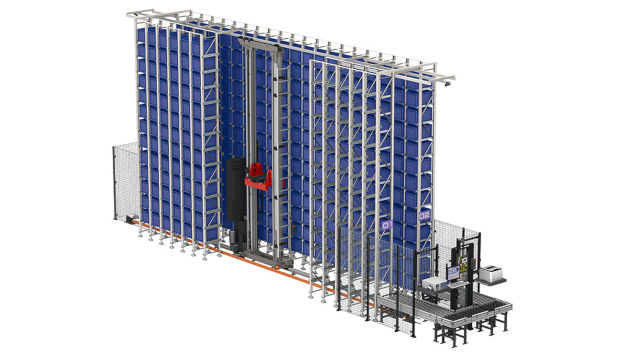
\includegraphics[width=0.7\linewidth]{images/miniload-asrs.jpg}
    \caption{AS/RS amb transelevador tipus miniload \cite{asrs_daifuku}.}
    \label{fig:transelevador1}
\end{figure}


\subsection{Contextos d'aplicació dels sistemes AS/RS}
Els sistemes AS/RS (\textit{Automated Storage and Retrieval Systems}) són sistemes d'emmagatzematge automatitzat controlats per ordinador, utilitzats en entorns industrials i logístics per gestionar el flux de materials de manera eficient. Aquests sistemes s'apliquen principalment en dos grans àmbits \cite{asrs_daifuku}:

\begin{itemize}
    \item \textbf{Indústria de fabricació}:
    \begin{itemize}
        \item Emmagatzematge de matèries primeres
        \item Subministrament de components a línies de producció
        \item Gestió de productes en procés (buffers)
        \item Emmagatzematge de producte final
    \end{itemize}

    \item \textbf{Logística i distribució}:
    \begin{itemize}
        \item Emmagatzematge temporal de productes
        \item Preparació de comandes
        \item Classificació i agrupació de mercaderies per a enviament
    \end{itemize}
\end{itemize}

Els AS/RS permeten un ús eficient de l'espai vertical del magatzem, incrementant la densitat d'emmagatzematge i millorant la gestió de l'inventari.

A més, contribueixen a la reducció de costos laborals, a la millora de la seguretat i a una major precisió en les operacions logístiques.



\subsection{Funcionament del transelevador}

El funcionament d'un transelevador \cite{transelevador_info} basa en un sistema automatitzat capaç de realitzar moviments coordinats per accedir a qualsevol posició dins del magatzem.

Aquest sistema opera principalment mitjançant tres moviments:

\begin{itemize}
    \item \textbf{Moviment longitudinal}: desplaçament al llarg del passadís sobre rails.
    \item \textbf{Moviment vertical}: elevació i descens de la càrrega mitjançant el màstil.
    \item \textbf{Moviment de càrrega}: introducció o extracció de la unitat de càrrega dins de l'estanteria.
\end{itemize}


En sistemes més avançats, els transelevadors es coordinen amb altres equips com cintes transportadores o sistemes de llançadora, integrant-se en un sistema logístic completament automatitzat. Aquests sistemes poden operar amb diferents tipus de càrrega, permetent adaptar el sistema a diferents necessitats industrials:

\begin{itemize}
    \item \textbf{Càrrega unitària}: palets o elements pesants.
    \item \textbf{Minicàrrega}: caixes, contenidors o productes lleugers.
\end{itemize}

\subsection{Parts principals d'un transelevador}

Un transelevador està format per diferents subsistemes mecànics i electrònics que permeten el seu funcionament automatitzat dins del magatzem (Figura \ref{fig:parts_transelevador}).

Entre els principals elements \cite{transelevador_info} que el componen destaquen:

\begin{itemize}
    \item \textbf{Sistema de presa de càrrega}: habitualment una pinça o plataforma elevadora que permet la manipulació de la unitat de càrrega dins de les estanteries.

    \item \textbf{Sistema de sensors}: conjunt de dispositius encarregats de detectar la posició, presència de càrrega i estat del sistema, essencials per al control automàtic.

    \item \textbf{Sistemes d'accionament}: motors elèctrics que permeten els moviments principals del transelevador(vertical, horitzonatl i transversal):

    \item \textbf{Sistema de manipulació extensible}: mecanismes que permeten introduir i extreure la càrrega de les estanteries.

    \item \textbf{Estructura mecànica}: formada per màstil o columna, xassís superior i inferior, i sistemes de guia sobre rails.

    \item \textbf{Unitat d'elevació}: inclou la cuna o plataforma elevadora, motor d'elevació i sistemes de seguretat associats.

    \item \textbf{Unitat de traslació}: permet el moviment longitudinal mitjançant rodes sobre rails, amb sistemes anti-descarrilament.

    \item \textbf{Sistema elèctric}: armari elèctric, sistemes d'alimentació i protecció.

    \item \textbf{Sistema de control}: pot ser manual (cabina d'operador) o automàtic mitjançant sistemes basats en microprocessadors.

    \item \textbf{Punt de comandament}: pot ser embarcat, remot o d'emergència.
\end{itemize}

Aquests sistemes treballen conjuntament per permetre el moviment eficient de càrregues en passadissos estrets i a gran altura.

\begin{figure}[H] 
    \centering
    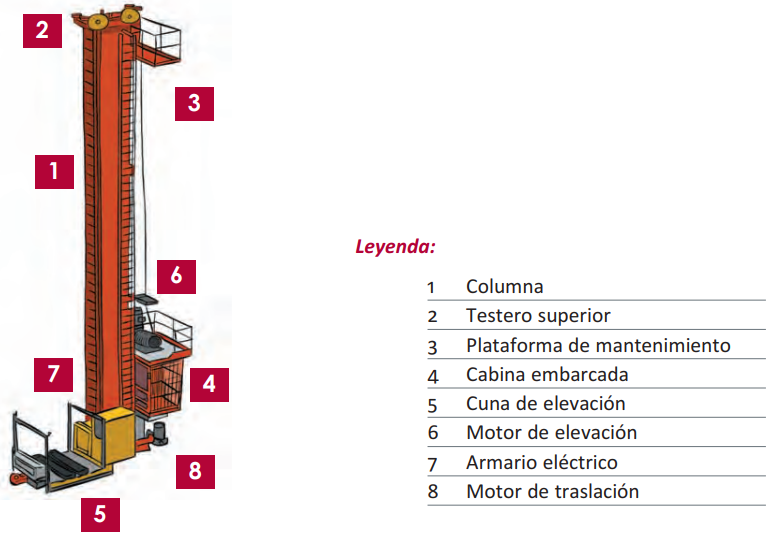
\includegraphics[width=0.5\linewidth]{images/parts_trans.PNG}
    \caption{Parts principals d'un transelevador industrial \cite{manual_logistica}.}
    \label{fig:parts_transelevador}
\end{figure}

\subsection{Normativa i estanteries en sistemes AS/RS}

Els transelevadors són equips industrials automatitzats que han de complir diferents normatives de seguretat i disseny, tant a nivell europeu com estatal.

Les principals normatives aplicables \cite{manual_logistica} són:

\begin{itemize}
    \item \textbf{Directiva 2006/42/CE}: regula els requisits de seguretat en el disseny de màquines.
    \item \textbf{Reial Decret 1215/1997}: estableix les condicions de seguretat en l'ús d'equips de treball.
    \item \textbf{UNE-EN 528}: norma específica per a transelevadors.
    \item \textbf{UNE-EN 1090-1}: relacionada amb estructures metàl·liques.
\end{itemize}

A més, aquests sistemes requereixen documentació tècnica obligatòria, com el manual d'instruccions, certificat CE, resultats d'assajos i registres d'inspecció.

\subsubsection{Norma UNE-EN 15620 i classificació d'estanteries}

El disseny del sistema també depèn de les estanteries utilitzades \cite{rack_estanterias_norma}. La norma \textbf{UNE-EN 15620} defineix toleràncies i precisió en sistemes d'emmagatzematge.

Segons aquesta norma, les estanteries es classifiquen en:

\begin{itemize}
    \item \textbf{Classe 100}: transelevadors automàtics en instal·lacions estàndard (altura inferior a 18m).
    \item \textbf{Classe 200}: major precisió amb sistemes de posicionament comparat amb la classe 100.
    \item \textbf{Classe 300A}: passadissos molt estrets amb operació guiada.
    \item \textbf{Classe 300B}: similar però amb menor assistència.
    \item \textbf{Classe 400}: sistemes manuals amb carretons convencionals.
\end{itemize}

Aquesta classificació és clau per determinar el nivell d'automatització i precisió del sistema.

\begin{figure}[H]
    \centering
    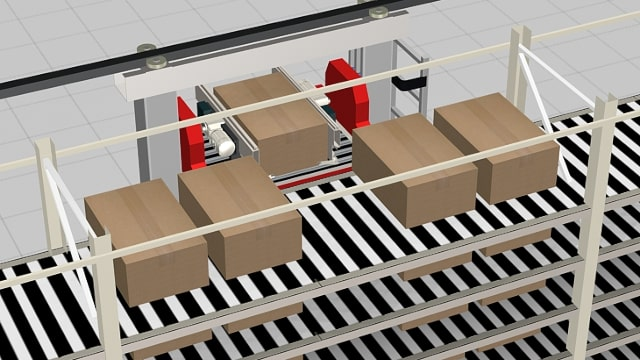
\includegraphics[width=0.45\linewidth]{images/shelving-rack.jpg}
    \caption{Exemple d'estanteries per a sistemes automatitzats tipus miniload \cite{asrs_daifuku}}
\end{figure}


\subsection{Seguretat en els transelevadors}
Els transelevadors operen en entorns automatitzats amb moviments d'alta velocitat i manipulació de càrregues, fet que implica riscos que han de ser controlats adequadament.

Els principals riscos associats inclouen:
\begin{itemize}
    \item Aplastament per impacte amb estructures
    \item Caiguda de càrregues
    \item Contactes elèctric
    \item Caigudes en operacions de manteniment
    \item Errors de control del sistema
\end{itemize}

Per minimitzar aquests riscos \cite{manual_logistica}, els sistemes incorporen diferents mesures de seguretat com ara \textbf{parades d'emergència} accessibles, \textbf{control d'accés} mitjançant enclavaments, \textbf{sensors} de seguretat i finals de carrera, així com \textbf{sistemes anti-caiguda} i \textbf{reguladors de velocitat}.

A nivell de disseny, també s'integren dispositius com sistemes antidescarrilament, frenada automàtica en cas de fallada d'energia i limitadors de recorregut i velocitat.

Finalment, el sistema de control evita canvis de mode no autoritzats i garanteix la coherència entre accessos i comandaments, assegurant un funcionament segur en tot moment.


\subsection{Condicions d'ús i manteniment}

Els transelevadors són equips sotmesos a un ús intensiu i continu, especialment en sistemes automatitzats, per la qual cosa requereixen un manteniment adequat i un control estricte del seu estat.

Segons la normativa aplicable \cite{manual_logistica}, aquests equips han de sotmetre's a inspeccions periòdiques realitzades per personal autoritzat. Entre els aspectes clau destaquen:

\begin{itemize}
    \item Inspeccions periòdiques segons el manual del fabricant
    \item Revisió anual d'almenys el 20\% de la instal·lació
    \item Inspecció completa cada 5 anys
    \item Assajos funcionals amb càrrega nominal i addicional
\end{itemize}

El manteniment inclou:

\begin{itemize}
    \item Substitució preventiva de components
    \item Lubricació d'elements mecànics
    \item Control de sistemes de seguretat
    \item Verificació del correcte funcionament dels sensors i actuadors
\end{itemize}

Pel que fa a les condicions d'ús:

\begin{itemize}
    \item L'operador ha de ser major d'edat, format i autoritzat
    \item S'ha de registrar qualsevol incidència o avaria
    \item No es permet l'accés a persones als passadissos durant el funcionament
    \item S'han de seguir protocols estrictes en operacions de manteniment
\end{itemize}

Finalment, és obligatori disposar de procediments d'emergència i realitzar simulacres periòdics per garantir una resposta adequada davant possibles fallades del sistema.

\subsection{Relació del sistema desenvolupat amb els sistemes AS/RS i transelevadors}

El sistema desenvolupat en aquest treball es pot classificar conceptualment com un sistema AS/RS de tipus minicàrrega \cite{asrs_daifuku}, ja que implementa una gestió automatitzada del flux de materials, incloent transport, emmagatzematge i evacuació de peces.

Un dels elements clau és la utilització de transelevadors, que reprodueixen el comportament típic d'aquests equips industrials mitjançant moviments coordinats en eixos vertical i horitzontal per posicionar càrregues en diferents nivells d'estanteria.

A més, el sistema integra característiques pròpies dels AS/RS reals, com ara l'automatització del procés, el control de posició mitjançant sensors i la gestió estructurada de l'emmagatzematge.

Tot i això, cal destacar que es tracta d'un model simplificat respecte a instal·lacions industrials reals (Figura \ref{fig:comparacion_asrs}). Per exemple, no s'inclouen aspectes com la gestió multi-passadís, sistemes redundants, optimització avançada de rutes o integració amb sistemes ERP. Una descripció detallada del funcionament i de la implementació del sistema es presenta a la secció \ref{sec:disseny_proces}.

\begin{figure}[H]
\centering

\begin{minipage}{0.42\textwidth}
    \centering
    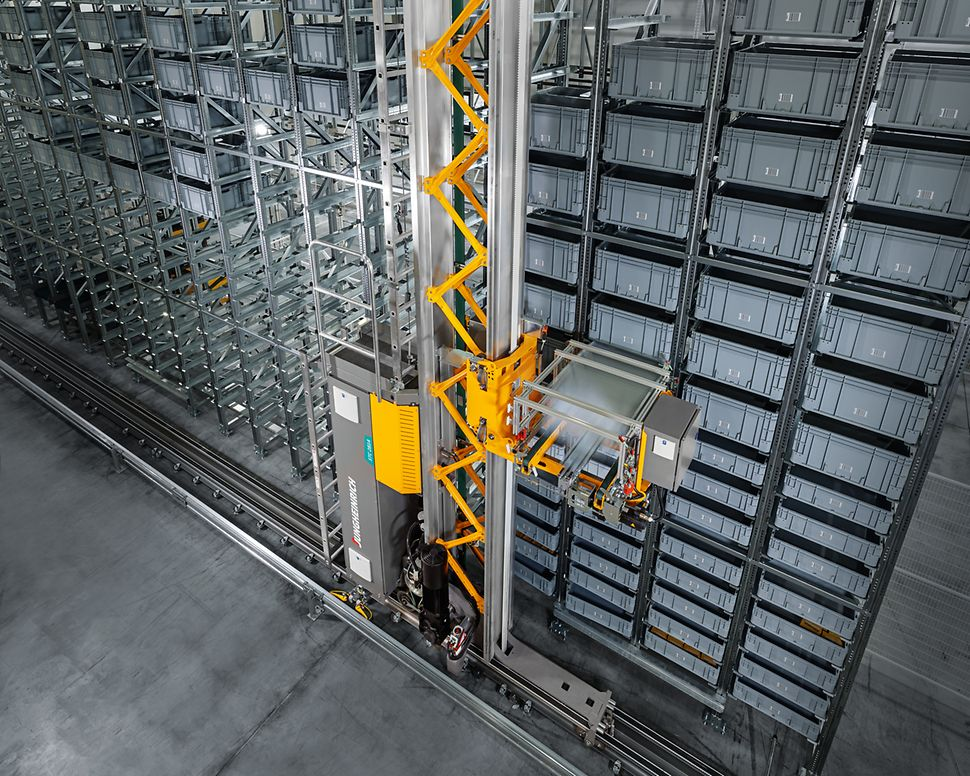
\includegraphics[width=\linewidth]{images/stage-miniload.jpg}
    \caption*{Sistema AS/RS industrial amb transelevador real \cite{transelevadores_jungheinrich}}  
\end{minipage}
\hfill
\begin{minipage}{0.42\textwidth}
    \centering
    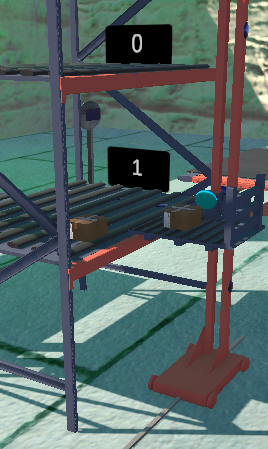
\includegraphics[width=0.5\linewidth]{images/unity_transelevador.png}
    \caption*{Model desenvolupat en Unity del sistema implementat}
\end{minipage}

\caption{Comparació entre AS/RS real i el model desenvolupat en aquest projecte}
\label{fig:comparacion_asrs}
\end{figure}

\newpage
\section{Disseny del procés industrial i arquitectura de comunicació}
\label{sec:disseny_proces}
%%\subsection{Concepció general del sistema}

La planta industrial dissenyada com a simulació d'una planta industrial dintre de Unity representa un sistema automatitzat de classificació i emmagatzematge de peces. La lògica del procés s'executa íntegrament en Unity, mentre que Rapid SCADA actua com a sistema de supervisió, monitoratge i enviament de comandes d'operació.

Aquesta separació és intencionada i respon a criteris d'arquitectura industrial moderna:

\begin{itemize}
\item Unity = sistema físic simulat + lògica de control.
\item Rapid SCADA = capa de supervisió i operació.
\item MQTT = canal de comunicació desacoblat.
\end{itemize}

Aquest enfocament permet reproduir una arquitectura equivalent a la d'un sistema industrial real on el PLC executaria la lògica i el SCADA supervisaria el procés.

\subsection{Disseny detallat del procés industrial}
El sistema industrial virtual que finalment s'ha decidit realitzar en l'entorn virtual ha anat evolucionant cap a una arquitectura més complexa basada en sistemes d'emmagatzematge automatitzat similars als utilitzats en magatzems industrials tipus AS/RS.

El procés consta de tres subsistemes principals:

\begin{itemize}
\item Sistema d'entrada i classificació inicial.
\item Sistema d'emmagatzematge amb transelevador.
\item Sistema d'evacuació amb transelevador de sortida.
\end{itemize}


%%\subsubsection{Descripció funcional global}

El sistema simula una línia automatitzada de classificació, emmagatzematge i evacuació de peces, diferenciades en tres tipus (A $\rightarrow$ Cub, B $\rightarrow$ Cilindre vertical i C $\rightarrow$ Triangle). El procés es desenvolupa de manera seqüencial seguint les etapes següents:

\subsubsection*{1. Generació i transport inicial}

Les peces són generades sobre la cinta principal (motor M1), que les transporta cap a la zona de control. El sensor S1 detecta la presència de peça i inicia el procés.

\subsubsection*{2. Identificació de tipus}

A la zona d'identificació, el sensor S2 determina el tipus de peça segons la seva geometria:

\begin{itemize}
\item Peça A (cub) = 1
\item Peça B (cilindre vertical) = 2
\item Peça C (triangle) = 3
\end{itemize}

Aquesta informació s'utilitza per definir la seva destinació dins del sistema.

\subsubsection*{3. Transferència i elevació}

La peça és transferida al primer transelevador, que la posiciona segons el tipus detectat al lloc predeterminat. Consta d'un sensor de presència (\textbf{S3}) per detectar si la peça ha arribat correctament a la plataforma d'elevació. Aquest sistema combina:
\begin{itemize}
\item Moviment vertical (3 possibles nivells d'estanteria i el nivell de la cinta) 
\item Moviment horitzontal (3 possibles posicions dins l'estanteria i la posició de la cinta) 
\end{itemize}

Els sensors de posició permeten conèixer en tot moment la ubicació del transelevador i garantir un posicionament correcte, tant verticalment com horitzontalment.

\subsubsection*{4. Dipòsit en estanteria}

Un cop el transelevador es troba a la posició corresponent, la peça es diposita a l'estanteria mitjançant els rodets de la plataforma del transelevador (M4). 

Cada estanteria està associada a un tipus de peça i disposa de diverses posicions. Les peces s'organitzen de manera progressiva, desplaçant-se cap a l'interior per deixar espai a noves entrades.


Per garantir el control correcte de l'estat de cada zona d'emmagatzematge, s'han distribuït sensors de presència en cadascun dels nivells, permetent detectar l'ocupació de les diferents posicions. Addicionalment, cada nivell incorpora sistemes de rodets motoritzats que faciliten tant la inserció de noves peces com el procés posterior d'evacuació.

Quan una estanteria arriba a la seva capacitat màxima (nou peces en aquest cas), el sistema inicia automàticament el procés d'evacuació de les peces emmagatzemades cap a la zona de sortida de la planta.

\subsubsection*{5. Evacuació per estanteria plena}


Quan una estanteria arriba a la seva capacitat màxima, s'activa el procés d'evacuació. Les peces són transportades cap a un segon transelevador, encarregat de recollir-les.

Aquest segon transelevador és l'encarregat de transportar les peces des de les estanteries fins a la cinta d'evacuació final. Per fer-ho, disposa d'una plataforma amb rodets motoritzats que permeten introduir i extreure les caixes de manera automàtica.

A diferència del primer transelevador, aquest sistema disposa de dues posicions horitzontals -corresponents a la zona d'estanteries i a la cinta d'evacuació- i quatre posicions verticals -associades als tres nivells d'estanteria i al nivell de la cinta de sortida. Cada posició es troba monitoritzada mitjançant sensors, permetent conèixer en tot moment la ubicació exacta del transelevador.

\subsubsection*{6. Evacuació final}
Quan el segon transelevador està completament carregat amb nou caixes, es desplaça fins a la posició final on es troba la cinta d'evacuació. Se sap si el transelevador està completament carregat gràcies a disposar de dos sensors de prescència, al final i al principi de la plataforma. Quan els dos es troben actius, s'assumeix que està carregada adequadament.

En aquest punt, totes les peces de la plataformes són expulsades simultàniament gràcies als rodets de la plataformes cap a la cinta d'evacuació, qui serà l'encarregat d'enviar les peces fora de la planta industrial.

\subsubsection{Taula de sensors, actuadors i comptadors del sistema}
\label{sec:tables}
A continuació es mostra la llista completa de sensors i actuadors utilitzats en la planta industrial virtual.

\begin{table}[H]
\centering
\small

\caption{Sensors del sistema}
\label{tab:tab_sensors}
\begin{tabular}{|p{3cm}|p{5cm}|p{6cm}|}

\hline
\textbf{Sensor} & \textbf{Ubicació} & \textbf{Funció} \\ \hline

S1 & Cinta principal & Detecta la presència de peça a l'entrada del sistema \\ \hline
S2 & Estació d'identificació & Determina el tipus de peça (A, B o C) \\ \hline
S3 & Plataforma transelevador 1 & Detecta presència de caixa a la plataforma \\ \hline
S4 & Transelevador 1 & Posició horitzontal a cinta principal \\ \hline
S5 & Transelevador 1 & Posició horitzontal 1 davant estanteries \\ \hline
S6 & Transelevador 1 & Posició horitzontal 2 davant estanteries \\ \hline
S7 & Transelevador 1 & Posició horitzontal 3 davant estanteries \\ \hline
S8 & Transelevador 1 & Posició vertical nivell cinta \\ \hline
S9 & Transelevador 1 & Posició vertical nivell estanteria A \\ \hline
S10 & Transelevador 1 & Posició vertical nivell estanteria B \\ \hline
S11 & Transelevador 1 & Posició vertical nivell estanteria C \\ \hline
S12 & Cinta evacuació final & Detecta presència de caixa evacuada \\ \hline
S13 & Plataforma transelevador 1 & Detecta presència de caixa al principi de la plataforma \\ \hline
S14 & Plataforma transelevador 1 & Detecta presència de caixa  al final de la plataforma \\ \hline

SA\_1$\rightarrow$SA\_3 & Estanteria A & Sensor presència caixa posició 1 $\rightarrow$posició 3  \\ \hline
SB\_1$\rightarrow$SB\_3 & Estanteria B & Sensor presència caixa posició 1$\rightarrow$posició 3  \\ \hline
SC\_1$\rightarrow$SC\_3 & Estanteria C & Sensor presència caixa posició 1$\rightarrow$posició 3\\ \hline

SH\_1 & Transelevador 2 & Posició horitzontal 1 \\ \hline
SH\_2 & Transelevador 2 & Posició horitzontal 2 \\ \hline

SV\_1 & Transelevador 2 & Posició vertical nivell 1 (cinta evacuació)\\ \hline
SV\_2 & Transelevador 2 & Posició vertical nivell 2 (estanteria A)\\ \hline
SV\_3 & Transelevador 2 & Posició vertical nivell 3 (estanteria B)\\ \hline
SV\_4 & Transelevador 2 & Posició vertical nivell 4 (estanteria C)\\ \hline

\end{tabular}


\end{table}

\begin{table}[H]
\centering
\small

\caption{Actuadors del sistema}
\label{tab:tab_actuadors}
\begin{tabular}{|p{3cm}|p{5cm}|p{6cm}|}

\hline
\textbf{Motor} & \textbf{Ubicació} & \textbf{Funció} \\ \hline

M1 & Cinta principal & Transport de peces a l'entrada del sistema \\ \hline
M2 & Transelevador 1 & Moviment horitzontal del transelevador \\ \hline
M3 & Transelevador 1 & Moviment vertical del transelevador \\ \hline
M4 & Plataforma transelevador 1 & Rodets per introduir o extreure caixes \\ \hline
M5 & Transelevador 2 & Moviment horitzontal \\ \hline
M6 & Transelevador 2 & Moviment vertical \\ \hline
M7 & Plataforma transelevador 2 & Rodets moviment de caixes \\ \hline
M8 & Cinta evacuació final & Transport de caixes fora del sistema \\ \hline
M9\_A & Estanteria A & Motor dels rodets \\ \hline
M9\_B & Estanteria B & Motor dels rodets \\ \hline
M9\_C & Estanteria C & Motor dels rodets \\ \hline

\end{tabular}

\end{table}

\begin{table}[H]
\centering
\small
\caption{Comptadors del sistema}
\label{tab:tab_comptadors}
\begin{tabular}{|p{3cm}|p{5cm}|p{6cm}|}
\hline
\textbf{Comptador} & \textbf{Ubicació / Associació} & \textbf{Funció} \\ \hline

C\_A & Estanteria A & Registra el nombre actual de peces de tipus A emmagatzemades \\ \hline

C\_B & Estanteria B & Registra el nombre actual de peces de tipus B emmagatzemades \\ \hline

C\_C & Estanteria C & Registra el nombre actual de peces de tipus C emmagatzemades \\ \hline

Count\_EvacA & Sistema d'evacuació & Comptabilitza el total de peces de tipus A evacuades del sistema \\ \hline

Count\_EvacB & Sistema d'evacuació & Comptabilitza el total de peces de tipus B evacuades del sistema \\ \hline

Count\_EvacC & Sistema d'evacuació & Comptabilitza el total de peces de tipus C evacuades del sistema \\ \hline

\end{tabular}

\end{table}

\subsection{Modelització segons filosofia GEMMA}

La filosofia GEMMA (\textit{Guide d'Étude des Modes de Marches et d'Arrêts}) és una metodologia utilitzada en automatització industrial per definir de manera estructurada els diferents modes de funcionament i aturada d'un sistema automàtic. Aquesta metodologia permet establir un comportament coherent i segur del sistema davant situacions normals d'operació, parades controlades, funcionament manual o situacions d'emergència.

En aquest projecte, la filosofia GEMMA s'ha utilitzat com a base per definir els principals estats de funcionament de la planta industrial virtual desenvolupada a Unity i supervisada mitjançant Rapid SCADA. Els modes implementats dins del sistema són els següents:
\begin{itemize}
\item A1 - Estat inicial segur: Tots els actuadors desactivats. Elevadors en posició segura. Sensors desactivats.

\item F1 - Producció automàtica: Execució contínua del cicle complet de classificació sense intervenció de l'operador.

\item F5 - Funcionament manual: L'operador pot activar individualment motors i pistons.

\item A2 - Aturada a final de cicle: El sistema es pararà després d'haver acabat el cicle que es troba fent.
\item A3 - Pausa: El procès es pararà en l'estat en el que es trobi.
\item D1 - Aturada d'emergència: Tall immediat de tots els actuadors. Prioritat absoluta de seguretat.

\item D2 - Tractament d'avaria: Permet diagnòstic i rearmament controlat.
\end{itemize}

\subsection{Especificació dels topics MQTT}

La comunicació entre Unity i RapidSCADA es basa en una arquitectura Publish/Subscribe mitjançant MQTT \cite{Team2015MQTT}. Cada topic representa una variable concreta del sistema. Totes les dades transmeses són de tipus enter (\textit{int}). La interpretació del valor és acordada prèviament entre ambdós sistemes i forma part del disseny del protocol intern. No s'utilitzen dades en format text per garantir compatibilitat amb entorns industrials reals i facilitar una possible integració amb PLCs.
\subsubsection{Estructura general dels topics}

Els topics segueixen la següent estructura:

\begin{itemize}
\item \textbf{plant/sensors/*} → Estat de sensors
\item \textbf{plant/actuators/*} → Estat d'actuadors
\item \textbf{plant/counters/*} → Comptadors
\item \textbf{plant/status/*} → Estat global
\item \textbf{plant/alarms/*} → Alarmes
\item \textbf{plant/cmd/*} → Ordres de control
\end{itemize}

\subsubsection{Topics de lectura i escriptura}


Aquests topics representen les variables de procés que Unity publica i Rapid SCADA llegeix per supervisar l'estat de la planta virtual.

\paragraph{Sensors}

Els sensors segueixen la nomenclatura: \textbf{plant/sensors/Si},  on \textit{i} correspon al número del sensor definit a la Taula \ref{tab:tab_sensors}.


\textbf{Convenció utilitzada:}

\begin{itemize}
\item 0 = sensor inactiu
\item 1 = sensor actiu
\end{itemize}

En el cas dels sensors d'identificació de peça, el valor representa el tipus de peça detectada:


\begin{itemize}
\item 0 = cap peça
\item 1 = peça tipus A
\item 2 = peça tipus B
\item 3 = peça tipus C
\end{itemize}
\paragraph{Actuadors}
Els actuadors segueixen la nomenclatura: \textbf{plant/actuators/Mi}, on \textit{i} correspon al número del motor o actuador definit a la Taula \ref{tab:tab_actuadors}.


\textbf{Convenció utilitzada:}

\begin{itemize}
\item 0 = actuador aturat
\item 1 = moviment o funcionament normal
\item -1 = moviment invers (només aplicable als rodets bidireccionals)
\end{itemize}


\paragraph{Comptadors}
Els comptadors segueixen la nomenclatura: \textbf{plant/counters/*}. La descripció detallada dels comptadors implementats es mostra a la Taula \ref{tab:tab_comptadors}.

\paragraph{Estat del sistema}

Les variables globals d'estat permeten conèixer el mode actual de funcionament del sistema. El topic \textbf{plant/status/actuation mode} indica el mode de control actual, seguint la convenció definida a continuació:

\textbf{Convenció utilitzada:}

\begin{itemize}
\item -1 = Aturat
\item 0 = Automàtic
\item 1 = Manual
\end{itemize}


\paragraph{Alarmes}

Les alarmes permeten indicar situacions de seguretat o fallada del sistema.

\textbf{Convenció utilitzada:}

\begin{itemize}
\item 0 = Funcionament normal
\item 1 = Emergència activa
\end{itemize}

\subsubsection{Topics de control (SCADA $\rightarrow$ Unity)}
Aquests topics representen les ordres enviades des de Rapid SCADA cap a Unity per controlar el comportament de la planta virtual.

\textbf{Control general}

\begin{table}[H]
\centering
\small
\caption{Topics de control general}
\label{tab:mqtt_general_cmd}
\begin{tabular}{|p{5cm}|p{8cm}|}
\hline
\textbf{Topic} & \textbf{Funció} \\ \hline

plant/cmd/start & Inici del sistema \\ \hline

plant/cmd/stop & Aturada controlada \\ \hline

plant/cmd/reset & Reinicialització del sistema \\ \hline

plant/cmd/pause & Pausa temporal del procés \\ \hline

plant/cmd/emergency & Activació d'aturada d'emergència \\ \hline

\end{tabular}

\end{table}

\textbf{Convenció utilitzada:}

\begin{itemize}
\item 0 = ordre inactiva
\item 1 = ordre activada
\end{itemize}

\textbf{Selector de mode}

\begin{table}[H]
\centering
\small
\caption{Selector de mode de funcionament}
\label{tab:mqtt_selector}
\begin{tabular}{|p{5cm}|p{8cm}|}
\hline
\textbf{Topic} & \textbf{Convenció} \\ \hline

plant/cmd/selector &
-1 = STOP \newline
0 = AUTO \newline
1 = MANUAL \\ \hline

\end{tabular}

\end{table}

\paragraph{Control manual d'actuadors}

Els actuadors controlats manualment segueixen la nomenclatura \textbf{plant/cmd/Mi} on \textit{i} correspon al motor o actuador associat.


\textbf{Convenció utilitzada:}

\begin{itemize}
\item 0 = aturat
\item 1 = moviment endavant
\item -1 = moviment invers (en el cas dels rodets bidireccionals)
\end{itemize}

\paragraph{Control de posicionament dels transelevadors}

A diferència de la resta d'actuadors, els transelevadors funcionen mitjançant control per posició discreta. El valor enviat no representa directament el moviment, sinó la posició objectiu que ha d'assolir el sistema.

\begin{table}[H]
\centering
\small
\caption{Control de posicionament dels transelevadors}
\label{tab:mqtt_asrs}
\begin{tabular}{|p{4cm}|p{4cm}|p{5cm}|}
\hline
\textbf{Actuador} & \textbf{Topic} & \textbf{Valors vàlids} \\ \hline

Transelevador 1 horitzontal & plant/cmd/M2 & Posicions 1 a 4 \\ \hline

Transelevador 1 vertical & plant/cmd/M3 & Posicions 1 a 4 \\ \hline

Transelevador 2 horitzontal & plant/cmd/M5 & Posicions 1 a 2 \\ \hline

Transelevador 2 vertical & plant/cmd/M6 & Posicions 1 a 4 \\ \hline

\end{tabular}

\end{table}

El sistema interpreta aquests valors com a consignes de posició i la lògica interna s'encarrega de gestionar automàticament el moviment fins arribar al destí indicat.

\paragraph{Control manual de comptadors}

A diferència de la resta d'actuadors, els comptadors de producció i evacuació es poden modificar manualment. Aquesta funcionalitat és útil en tasques de manteniment, proves o correcció manual de valors.


\begin{table}[H]
\centering
\small
\caption{Control manual de comptadors de producció}
\label{tab:mqtt_manual_counters}
\begin{tabular}{|p{6cm}|p{7cm}|}
\hline
\textbf{Topic} & \textbf{Funció} \\ \hline

plant/cmd/manual/countA & Modificació del comptador de peces tipus A \\ \hline

plant/cmd/manual/countB & Modificació del comptador de peces tipus B \\ \hline

plant/cmd/manual/countC & Modificació del comptador de peces tipus C \\ \hline

plant/cmd/manual/CEvacA & Modificació del comptador d'evacuació de peces tipus A \\ \hline

plant/cmd/manual/CEvacB & Modificació del comptador d'evacuació de peces tipus B \\ \hline

plant/cmd/manual/CEvacC & Modificació del comptador d'evacuació de peces tipus C \\ \hline
\end{tabular}
\end{table}

\textbf{Convenció utilitzada:}

\begin{itemize}
\item 1 = incrementa una unitat el comptador associat
\item 0 = reinicia el comptador a zero
\end{itemize}


\newpage
\section{Disseny i implementació de la planta virtual en Unity}

Una vegada definits el procés industrial i l'arquitectura de comunicació del sistema, es va procedir al desenvolupament de la planta virtual mitjançant el motor gràfic Unity.

Aquest apartat descriu les decisions de disseny preses durant la construcció dels diferents components del sistema, així com la manera en què s'han implementat els comportaments necessaris mitjançant scripts. Es farà referència als conceptes mencionats en la part de teoria de Unity (secció \ref{sec:unity_theory}).

L'objectiu principal d'aquesta implementació  era reproduir el comportament d'una petita planta industrial automatitzada intentant que tot tingui un semblant realista ja sigui en l'apartat visual, en la funcionalitat del sistema i en la simplicitat de simulació.

\subsection{Construcció de l'entorn de la planta} 

Per definir l'entorn de treball que representarà la planta industrial, es va construir una sala utilitzant objectes geomètrics bàsics del motor. Concretament, es van utilitzar quatre \texttt{Cube} per representar les parets, ajustant-ne la mida i posició per delimitar correctament l'espai de simulació. Per al sòl es va utilitzar un objecte \texttt{Plane}, que permet cobrir superfícies àmplies de manera eficient.

Pel que fa a la selecció dels materials, s'han tingut en compte criteris habituals en entorns industrials, com ara la resistència mecànica, la durabilitat davant del desgast, la facilitat de neteja i la seguretat (superfícies antilliscants) \cite{industrial_floor_molins,pavimentos_sika}.

En base a aquests criteris, els paviments industrials acostumen a utilitzar materials com el formigó polit, les resines epoxi o els paviments de poliuretà. En aquest projecte s'ha optat per una textura de \textbf{formigó polit} (Figura \ref{fig:formigo}). 

Pel que fa a les parets, en entorns industrials són comunes solucions com el maó, els panells metàl·lics o superfícies pintades. En aquest cas, s'ha seleccionat una textura de \textbf{maó pintat} (Figura \ref{fig:mao}).

\begin{figure}[H]
\centering
\begin{subfigure}{0.25\textwidth}
    \centering
    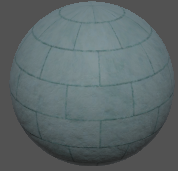
\includegraphics[width=\linewidth]{images/concrete_texture.png}
    \caption{Textura de formigó polit \cite{texture_concrete}}
    \label{fig:formigo}
\end{subfigure}
\hspace{3cm}
\begin{subfigure}{0.25\textwidth}
    \centering
    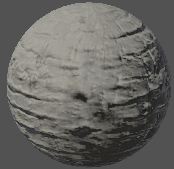
\includegraphics[width=\linewidth]{images/brick_texture.png}
    \caption{Textura de maó pintat \cite{texture_brick}}
    \label{fig:mao}
\end{subfigure}
\caption{Materials utilitzats per a la construcció de l'entorn industrial}
\end{figure}



\subsection{Models 3D utilitzats en la planta}

La major part dels elements mecànics de la planta no han estat modelats des de zero, sinó que s'han obtingut a partir de repositoris públics d'actius per a Unity. Això ha permès centrar el desenvolupament en la lògica del sistema i el comportament dels components.

Tot i això, la majoria dels models han estat adaptats per ajustar-los a les necessitats del projecte. Principalment, s'han modificat els materials originals per aconseguir una estètica més coherent amb l'entorn industrial definit.

En alguns casos concrets, com els transelevadors, els models 3D han estat editats mitjançant \textit{Blender} \cite{blender_download} per simplificar l'estructura, separar components i adaptar-los al comportament requerit dins de la simulació. De manera similar, les estanteries també han estat ajustades a partir del model base per millorar la seva funcionalitat dins del sistema. Els principals components utilitzats en la construcció de la planta són els següents. 

\begin{itemize}

\item \textbf{Conveyor:}  
La cinta utilitzada per l'entrada de peces es mostra a la figura  \ref{fig:conveyor1}

\begin{figure}[H]
    \centering
    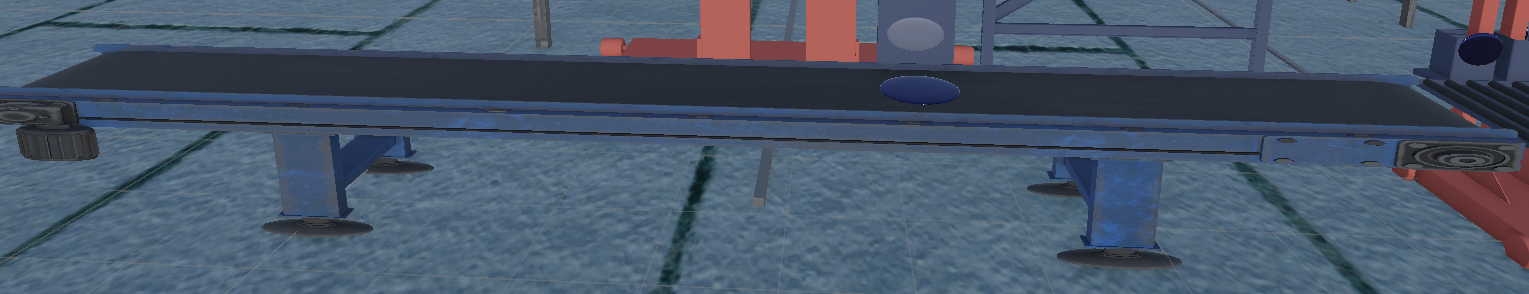
\includegraphics[width=0.7\linewidth]{images/conveyor1.png}
    \caption{Cinta principal. Autor:\textit{jkvarel} \cite{sketchfab_conveyor}}
    \label{fig:conveyor1}
\end{figure}


\item \textbf{Estanteria industrial - Warehouse Shelf Rack:}  
L'estructura d'emmagatzematge de peces es mostra a la figura \ref{fig:shelf}. Model proposat per l'autor \textit{scailman} \cite{sketchfab_warehouse}, però modificat per mi. 

\begin{figure}[H]
    \centering
    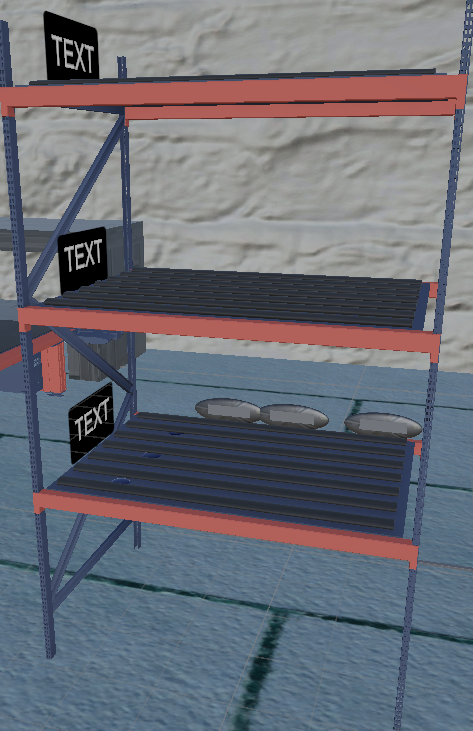
\includegraphics[width=0.35\linewidth]{images/shelf.png}
    \caption{Model estanteria}
        \label{fig:shelf}

\end{figure}


\item \textbf{Cinta transportadora d'evacuació - Conveyor Belt Assembly Line:}
Utilitzada en la fase final del procés per transportar les caixes fora del sistema (Figura \ref{fig:conveyor2}). 

\begin{figure}[H]
    \centering
    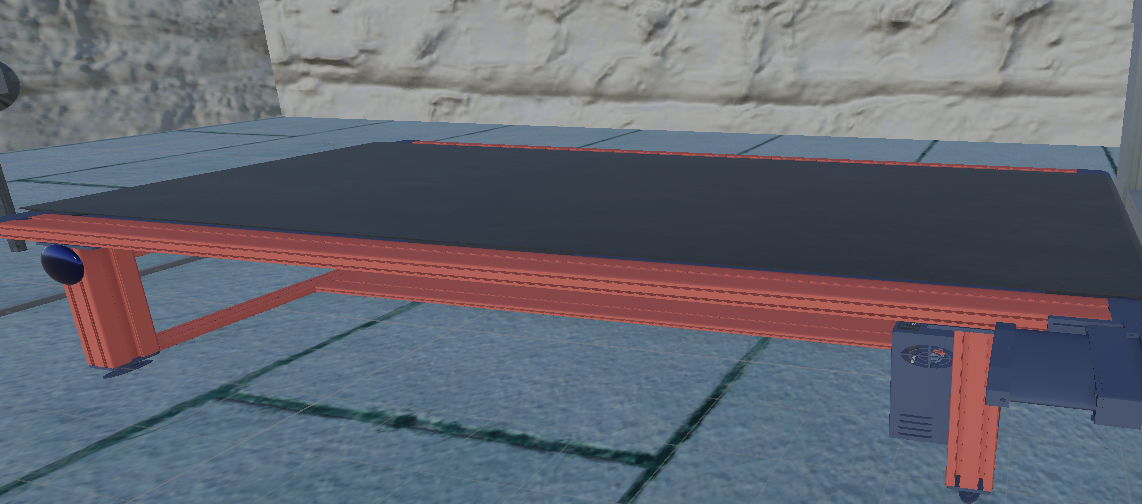
\includegraphics[width=0.5\linewidth]{images/conveyor2.png}
    \caption{Cinta evacuació. Autor: \textit{LOVANO} \cite{conveyor_assembly}}
        \label{fig:conveyor2}

\end{figure}

\item \textbf{Models de caixes - Card Boards Low Poly:} 

Models utilitzats per representar les peces que circulen pel sistema de producció (Figura \ref{fig:boxes}). Tant el cilindre com el triangle han estat creats a partir del model de caixa base mitjançant modificacions bàsiques en \textit{Unity}.
\begin{figure}[H]
    \centering
    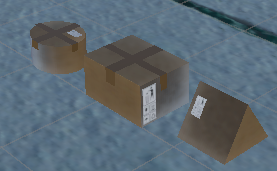
\includegraphics[width=0.3\linewidth]{images/pieces.png}
    \caption{Caixes utilitzades en el sistema. Autor: \textit{minitakesstudio} \cite{boxes_model}}
    \label{fig:boxes}
\end{figure}

\item \textbf{Transelevador - ASRS Concept:} 
Model utilitzat per representar el sistema automàtic d'emmagatzematge i recuperació de peces (Figura \ref{fig:transelevadors}). 

\begin{figure}[H]
\centering
\begin{subfigure}{0.3\textwidth}
    \centering
    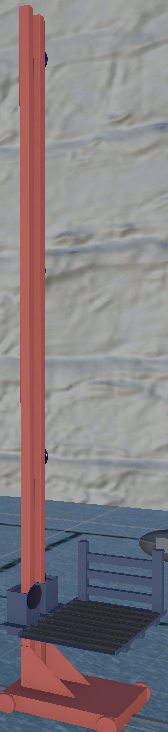
\includegraphics[width=0.355\linewidth]{images/transelevador1.png}
    \caption*{Transelevador 1}
\end{subfigure}
\hspace{1cm}
\begin{subfigure}{0.3\textwidth}
    \centering
    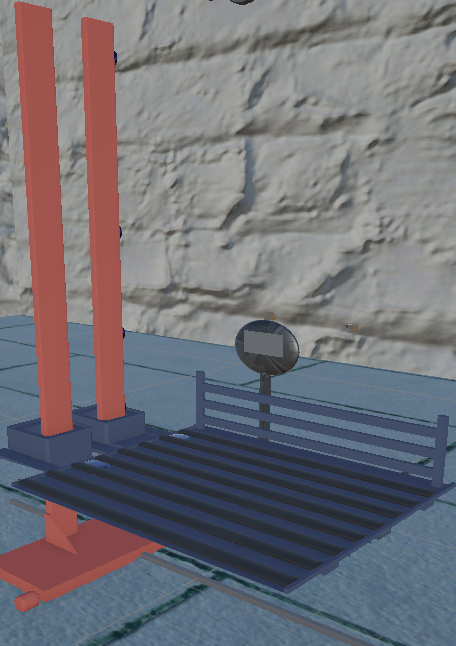
\includegraphics[width=\linewidth]{images/transelevador2.png}
    \caption*{Transelevador 2}
\end{subfigure}
\caption{Model transelevador, modificats per mi. Autor: \textit{Ford Jacobs} \cite{asrs_grabcad}}
    \label{fig:transelevadors}

\end{figure}


\item \textbf{Lamps:}
Models utilitzats per representar les llums de sistema correcta i d'emergència dintre de untiy (Figura \ref{fig:lamp}).

\begin{figure}[H]
\centering
\begin{subfigure}{0.2\textwidth}
    \centering
    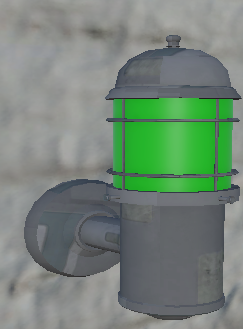
\includegraphics[width=\linewidth]{images/light_off.png}
    \caption*{Llum apagada}
\end{subfigure}
\hspace{1cm}
\begin{subfigure}{0.2\textwidth}
    \centering
    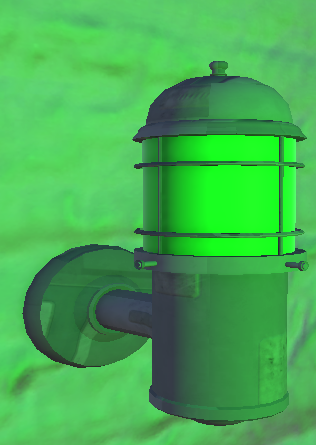
\includegraphics[width=\linewidth]{images/light_on.png}
    \caption*{Llum Encesa}
\end{subfigure}
\caption{Disseny de les làmpares i funcionalitat. Autor: \textit{Arrona72} \cite{wall_lamps}.}
    \label{fig:lamp}
\end{figure}

\end{itemize}

A més dels elements anteriors, s'han implementat també sensors virtuals que permeten detectar la presència de peces o la posició dels transelevadors en diferents punts del sistema.

\subsection{Sistema de control de càmera}

Per facilitar la navegació i inspecció de la planta virtual durant la simulació, s'ha implementat un sistema de control de càmera inspirat en el comportament de la vista d'escena de l'editor de Unity \cite{UnitySceneNavigation}. Aquest sistema permet a l'usuari moure's lliurement per l'entorn industrial, facilitant tant la supervisió del procés com les tasques de depuració i desenvolupament \cite{GameDeveloperCamera}.El comportament de la càmera es gestiona mitjançant l'script \textit{FreeCamera} (secció \ref{sec:scripts_unity}). Aquest script permet implementar tres funcionalitats principals:

\begin{itemize}
    \item \textbf{Rotació de càmera:} Quan es manté premut el botó dret del ratolí (\texttt{GetMouseButton(1)}), el sistema llegeix el moviment del ratolí mitjançant els eixos \texttt{Mouse X} i \texttt{Mouse Y} \cite{UnityInput}. A partir d'aquestes dades, es modifica la propietat \texttt{transform.eulerAngles}, permetent rotar la càmera al voltant dels eixos horitzontal i vertical. 
    \item \textbf{Desplaçament lateral (\textit{Panning}):} Quan es prem el botó central del ratolí (\texttt{GetMouseButton(2)}), la càmera es desplaça lateralment dins de l'escena. Aquest moviment es realitza utilitzant \texttt{transform.Translate()}, aplicant un desplaçament proporcional al moviment del ratolí i a la velocitat definida dintre del codi. D'aquesta manera, l'usuari pot moure's horitzontalment o verticalment sense modificar l'orientació de la càmera.
    \item \textbf{Zoom:} El zoom es controla mitjançant la roda del ratolí, llegint el valor de \texttt{MouseScrollWheel}. L'ús de \texttt{Space.Self} \cite{UnityTransformTranslate} permet que el moviment es realitzi segons l'orientació actual de la càmera, mantenint un comportament natural independentment de la seva rotació.
\end{itemize}


\subsection{Control de velocitat de la simulació}

Per facilitar les proves i l'anàlisi del comportament del sistema, s'ha implementat un mecanisme que permet modificar la velocitat global de la simulació en temps real mitjançant el teclat. El sistema utilitza la propietat \texttt{Time.timeScale} de Unity \cite{UnityTimeScale}, que permet accelerar o reduir la velocitat amb què s'executen tots els processos dependents del temps dins de la simulació (secció \ref{sec:scripts_unity}).

\begin{itemize}
\item En prémer la tecla \textbf{1}, la simulació funciona a velocitat normal.
\item En prémer la tecla \textbf{2}, la simulació funciona al doble de velocitat.
\item En prémer la tecla \textbf{3}, la simulació funciona cinc vegades més ràpid.
\end{itemize}

Aquest comportament és equivalent a l'opció d'accelerar la reproducció d'un vídeo. Tot el sistema continua funcionant amb la mateixa lògica i seqüència d'operacions, però els moviments, temporitzadors i processos es realitzen en menys temps.

\subsection{Implementació de les cintes transportadores}

Les cintes transportadores són un element clau del sistema, ja que permeten el desplaçament de les peces entre les diferents etapes del procés. Tot i utilitzar diferents models, totes les cintes comparteixen una estructura similar. Cada model inclou una part anomenada \textit{Belt}, que representa la superfície per on es mouen les peces i sobre la qual s'aplica el comportament funcional.  Per simular el moviment, s'han combinat dos mecanismes:

\begin{itemize}
\item \textbf{Moviment visual:} es desplaça l'\textit{offset} de la textura del material de la cinta en cada fotograma, generant la sensació de moviment continu. Aquesta part es realitza mitjançant el càlcul del paràmetre \texttt{mainTextureOffset} del material dins de la funció \texttt{Update()} (\cite{UnityUpdate}) de l'script associat a la cinta.
\item \textbf{Moviment físic:} s'aplica una velocitat als objectes situats sobre la cinta.
\end{itemize}

Per delimitar la zona de col·lisió amb els objectes (\textit{collider}), es disposa de dos colliders dintre del mateix objecte amb dues funcions: 

\begin{itemize}
\item Un \textbf{collider estàndard}, que manté les peces recolzades sobre la superfície.
\item Un \textbf{collider tipus \textit{trigger}} situat sobre el \textit{Belt}, que detecta les peces i permet aplicar el moviment a partir de la funció \texttt{OnTriggerStay}.
\end{itemize}

Per tal de controlar el comportament de la cinta s'hi ha aplicat un script (secció \ref{sec:scripts_unity}) a l'objecte \textit{Belt} que permetés controlar de forma independent el comportament de la superfície. Es recorda que un script és el codi que s'aplica a un component del sistema que li indica com ha de comportar-se dintre de la simulació. 

Per controlar la part del moviment, quan una peça amb etiqueta \textit{Box} \cite{UnityTags2023} entra al \text{trigger}, s'accedeix al seu \textit{Rigidbody} \cite{UnityRigidbody} i se li modifica el paràmetre de \texttt{linearVelocity}, aplicant un velocitat en la direcció de la cinta, modificant només les components horitzontals per no afectar la gravetat.

Per fer més accessible aquest codi, l'script incorpora mètodes públics per activar o desactivar la cinta i ajustar la seva velocitat, facilitant la seva integració dins de la lògica de control del sistema.

\subsection{Implementació del sistema d'estanteries}


El model 3D utilitzat per representar l'estructura d'emmagatzematge (\textit{Warehouse Shelf Rack}) no incorporava inicialment plataformes funcionals. Per aquest motiu, es va ampliar el model mitjançant la creació de nous objectes directament dins de Unity. Concretament, per cada nivell es van afegir plataformes com a \textit{subobjectes} de l'estructura principal, facilitant així la seva gestió dins de la jerarquia.

Cada plataforma disposa d'un \textbf{Box Collider} sense \textit{Trigger}, amb la funció de suportar físicament les caixes i evitar que travessin l'estructura durant la simulació.

\begin{figure}[H]
\centering
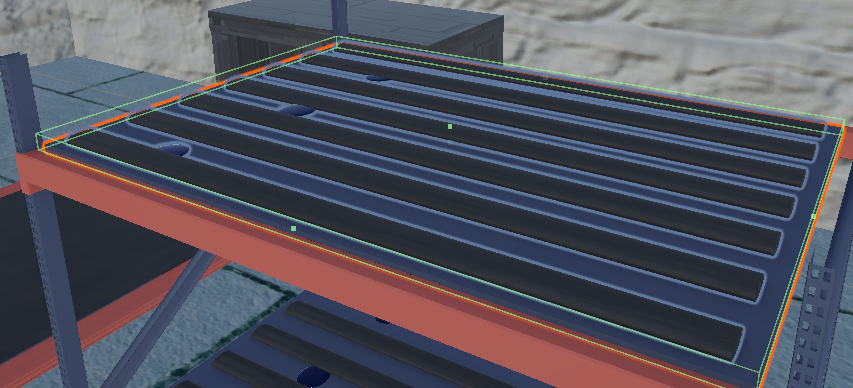
\includegraphics[width=0.7\textwidth]{images/collider_shelf.png}
\caption{Plataformes afegides a l'estanteria amb colliders}
\end{figure}

Addicionalment, s'ha implementat un sistema de rodets que permet reorganitzar les caixes dins de cada nivell quan una fila es completa. Aquest mecanisme desplaça les peces al llarg de la plataforma per deixar lliure la posició més propera al transelevador. El seu funcionament és equivalent al dels rodets de la plataforma del transelevador, que es descriu amb més detall en l'apartat \ref{sec:rollers}.

\subsection{Implementació del transelevador (ASRS Crane)}

El model original del sistema ASRS es trobava en format \textit{.stp}, per la qual cosa es va convertir a un format compatible amb Unity (\textit{.fbx}) \cite{stp_to_fbx}. A més a més, el model inicial presentava una estructura excessivament complexa per a la simulació, fet que va requerir la seva edició prèvia amb \textbf{Blender}. El programa Blender permet manipular models 3D de forma més precisa que Unity quan es tracta de separar malles, dividir objectes o reorganitzar l'estructura d'un model.

 Mitjançant aquest procés es van separar els diferents components del model, especialment els rodets de la plataforma, per tal de poder controlar-los de forma independent mitjançant \textit{scripts}. També es va afegir un \textit{Collider} a la plataforma per garantir el correcte suport de les peces durant el moviment.

\subsection*{Sistema de posicionament del transelevador}

El moviment del transelevador es basa en un conjunt de posicions predefinides mitjançant \texttt{Empty GameObjects} \cite{UnityGameObjects}, col·locats en els punts on el sistema ha d'aturar-se. Aquest enfocament permet definir les posicions de forma visual dins de Unity i simplifica la configuració del moviment. El \textbf{primer transelevador} disposa de 4 posicions horitzontals i 4 posicions verticals, mentre que el \textbf{segon transelevador} disposa de 2 posicions horitzontals i 4 posicions verticals.
Cada una d'aquestes posicions correspon a una localització específica del procés industrial, com ara la cinta principal, els diferents nivells d'estanteria o la zona d'evacuació.

\subsection*{Moviment horitzontal del transelevador}

El moviment horitzontal del transelevador es controla mitjançant un script específic que desplaça l'estructura del sistema entre les diferents posicions definides. L'script defineix les posicions objectiu i utilitza \texttt{Vector3.MoveTowards()} dins de \textit{FixedUpdate()} \cite{UnityUpdate} per desplaçar progressivament el transelevador. El moviment s'aplica mitjançant \textit{Rigidbody.MovePosition()}, garantint una integració correcta amb el sistema físic (secció \ref{sec:scripts_unity}).

\subsection*{Moviment vertical de la plataforma}

La plataforma del transelevador disposa d'un moviment vertical \cite{UnityElevatorVideo} independent que permet posicionar la càrrega als diferents nivells de l'estanteria (secció \ref{sec:scripts_unity}). En aquest cas, el moviment es calcula en coordenades locals (\textit{localPosition}) \cite{UnityTransformLocalPosition} per mantenir la coherència amb l'estructura jeràrquica del transelevador, ja que la plataforma és un objecte fill. Això evita desalineacions quan el conjunt es desplaça horitzontalment.

La nova posició es calcula amb \texttt{Vector3.MoveTowards()} i posteriorment es transforma a coordenades globals mitjançant \texttt{TransformPoint}, permetent l'ús de \texttt{Rigidbody.MovePosition()}.

El moviment s'executa dins de \texttt{FixedUpdate()}, garantint estabilitat en la simulació física. Degut a això, i al fet que el desplaçament es calcula de forma incremental, s'ha utilitzat una velocitat superior respecte al moviment horitzontal per mantenir una resposta visual coherent.

Finalment, el script incorpora la variable \textit{IsMoving}, que indica si la plataforma està en moviment. Aquesta informació és utilitzada per la lògica de control i per la seva integració amb el sistema SCADA.

\subsection*{Sistema de rodets de la plataforma}
\label{sec:rollers}
La plataforma del transelevador disposa d'un sistema de rodets que permet introduir o extreure les caixes. El seu funcionament és similar al d'una cinta transportadora, amb la diferència que pot operar en ambdues direccions (secció \ref{sec:scripts_unity}).  L'script detecta objectes amb \textit{Rigidbody} \cite{UnityRigidbody} dins d'un collider \textit{trigger} i aplica una velocitat en la direcció definida. Aquesta direcció es pot invertir mitjançant el paràmetre \textit{forward}.

Tanmateix, per reforçar l'efecte visual, s'ha implementat un script que desplaça la textura del material dels rodets (secció \ref{sec:scripts_unity}). Aquest només s'activa quan el sistema està en funcionament, mantenint coherència entre el moviment visual i físic.

\subsection{Indicadors visuals i sensors}

Per facilitar la visualització de l'estat del sistema, s'ha implementat un sistema d'indicadors visuals basat en LEDs virtuals, que reflecteixen l'estat dels sensors.

El comportament es gestiona mitjançant l'script \textit{LEDIndicator}, que canvia el material \cite{UnityMaterialsReference} de l'objecte segons l'estat del sensor associat (encès/apagat) (secció \ref{sec:scripts_unity}). Aquest enfocament permet desacoblar la lògica dels sensors de la seva representació visual, facilitant la reutilització del sistema.
%
%S'han implementat tres tipus de sensors que simulen el comportament de dispositius industrials reals:
%
%\begin{itemize}
%\item Sensors de presència
%\item Sensors òptics
%\item Sensors de posició
%\end{itemize}

\subsubsection{Sensors de presència}

Els sensors de presència s'utilitzen per detectar la presència de peces en punts concrets del sistema, com cintes o la plataforma del transelevador (secció \ref{sec:scripts_unity}).  Es basen en un \textit{Collider} en mode \textit{Trigger}, utilitzant els esdeveniments \texttt{OnTriggerEnter} i \texttt{OnTriggerExit} per detectar l'entrada i sortida d'objectes amb etiqueta \textit{Box} \cite{UnityColliders, UnityComponents}.

Per evitar errors amb múltiples peces simultànies, s'utilitza un comptador intern en lloc de \texttt{OnTriggerStay()}, reduint també el cost computacional. Quan una peça amb etiqueta \textit{Box} entra dins del sensor, aquest activa la variable interna del sensor i encén el LED associat.

\begin{figure}[H]
\centering
\begin{subfigure}{0.2\textwidth}
    \centering
    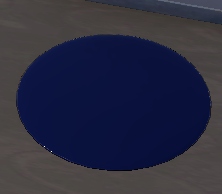
\includegraphics[width=\linewidth]{images/s1_off.png}
\end{subfigure}
\hspace{1cm}
\begin{subfigure}{0.2\textwidth}
    \centering
    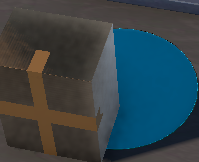
\includegraphics[width=\linewidth]{images/s1_on.png}
\end{subfigure}
\caption{Sensor de presència apagat i encès.}
\end{figure}

\subsubsection{Sensors òptics}

El sensor òptic permet identificar el tipus de peça mitjançant un script associat a cada objecte (secció \ref{sec:scripts_unity}).  Quan una peça entra dins del sensor, es llegeix aquesta informació i, després d'un retard controlat mitjançant un temporitzador, es valida la detecció (secció \ref{sec:scripts_unity}).  Aquest retard simula el temps de resposta d'un sensor real i permet al sistema prendre decisions en funció del tipus de peça. A l'apartat \ref{sec:timers} s'explica com s'ha implementat aquest retard. 

Com a implementació separada de la detecció bàsica, el sistema incorpora una simulació de fallades del sensor per tal d'aproximar el comportament del model a una situació industrial real. Per aconseguir-ho, s'ha implementat una probabilitat de fallada configurable mitjançant el paràmetre \texttt{failProbability}. Cada vegada que una peça és detectada correctament i finalitza el temporitzador del sensor, es genera un valor aleatori utilitzant \texttt{Random.value}. Si aquest valor és inferior a la probabilitat configurada, el sensor no detectarà la peça, provocant que el sistema entri en estat d'avaria.

Això permet generar situacions aleatòries d'error durant el funcionament de la simulació i comprovar la correcta resposta del sistema davant condicions no ideals.


\subsubsection{Sensors de posició del transelevador}

Els sensors de posició determinen la ubicació del transelevador mitjançant la comparació entre la seva posició actual i posicions de referència. Es basen en comparar la posició actual del transelevador amb la posició objectiu associada a cada sensor, calculant la distància entre el \textit{Rigidbody} i el punt de referència corresponent.

\begin{lstlisting}[style=simple]
public bool Pos1 => Vector3.Distance(rb.position, position1.position) <0.01f;
\end{lstlisting}

Quan la distància és inferior a un llindar, es considera que s'ha assolit la posició, activant també els indicadors LED associats a la vegada que s'activa la variable del sensor. Aquest sistema permet simular el comportament dels finals de carrera o sensors de posició utilitzats habitualment en sistemes AS/RS industrials.

\subsection{Sistema de llums d'estat}

S'ha implementat un sistema de llums \cite{UnityLighting}, basats en objectes \textbf{Point Light} de Unity (secció \ref{sec:lights}) per indicar l'estat global del sistema:

\begin{itemize}
\item Verd: funcionament automàtic
\item Vermell: estat d'emergència
\item Groc: mode manual
\end{itemize}

El control es realitza mitjançant variables com \textit{isOk}, \textit{emergency} i \textit{manual}. L'activació es fa habilitant o deshabilitant el \textit{GameObject} a través de la funció \texttt{SetActive()}, simulant l'encesa real (secció \ref{sec:lightsystem}). Per generar l'efecte intermitent de la llum vermella, s'utilitza un temporitzador basat en \texttt{Time.deltaTime}, que permet alternar l'estat de la llum de forma periòdica \cite{UnityTime}.

\subsection{Implementació d'un temporitzador (Timer)}
\label{sec:timers}


Per tal d'aproximar encara més el comportament del sistema a un entorn industrial real, s'ha implementat un mecanisme de temporització que permet introduir retards controlats en determinades accions del sistema. Aquest tipus de funcionalitat és especialment important en sistemes automatitzats, ja que molts processos industrials no es realitzen de manera instantània, sinó que requereixen un temps determinat per completar-se. 

Per implementar aquesta funcionalitat s'ha desenvolupat una classe anomenada \textit{Timer}, el funcionament de la qual és equivalent a un temporitzador de tipus \textbf{TON (Timer On Delay)} utilitzat habitualment en PLCs.

El funcionament d'aquest temporitzador (secció \ref{sec:scripts_unity}) es basa en una entrada booleana que activa el comptatge del temps mitjançant \texttt{Time.deltaTime} \cite{UnityTime}. Quan el temps acumulat supera el valor \texttt{preset} (valor predifinit del timer), la sortida \texttt{done} esdevé \texttt{true}. Si l'entrada es desactiva abans, el temporitzador es reinicia. Aquesta classe permet controlar de forma precisa els retards en la detecció de les peces del \textbf{sensor òptic}, així com en altres processos que requereixin una temporització específica dins del procès \textbf{d'automatització del sistema}.


\subsection{Interfície de visualització de dades (Canvas)}

A més dels indicadors LED, s'ha implementat una interfície gràfica en Unity per mostrar dades en temps real mitjançant el sistema \textit{Canvas} \cite{UnityCanvas}.

L'estructura es basa en un objecte pare amb vuit elements fills, on trobem quatra panells visuals i quatre elements de text. Tres d'aquests elements de text mostren el nombre de peces emmagatzemades. Un script \textit{DisplayCounter} (secció \ref{sec:scripts_unity}) actualitza aquest valor en cada fotograma accedint al comptador de caixes que es realitza en el procès automàtic i convertint-lo a text amb la funció \texttt{ToString()} \cite{dotnet_collections}. En canvi,el quart text mostra el tipus de peça detectada pel sensor òptic (secció \ref{sec:scripts_unity}). Quan no hi ha detecció es mostra \textit{"No piece"}, i en cas contrari es mostra el valor de l'enumeració \textit{PieceShape}.

S'ha utilitzat \textit{TextMeshPro} per a la representació del text, jofereix una qualitat de renderització de text superior en comparació amb el sistema de text tradicional, a part de més qualitat i de més flexibilitat. Els scripts treballen amb components \texttt{TMP\_Text} \cite{dotnet_text}, permetent actualitzar el contingut dinàmicament. 

\subsection{Generació i configuració de les peces del sistema}

Les peces constitueixen l'element principal que circula pel sistema industrial simulat, i per tant la seva correcta configuració és essencial per garantir un comportament físic i funcional adequat dins de l'entorn de Unity. Cada peça disposa de l'script \textit{PieceData} (secció \ref{sec:scripts_unity}), que defineix el seu tipus mitjançant una enumeració. A nivell físic \cite{UnityRigidbody}, totes les peces comparteixen:

\begin{itemize}

\item \textbf{Component Rigidbody} amb gravetat activada

\item \textbf{Restricció de rotacions en eix X i Z} per garantir estabilitat. 

\item \textbf{Etiqueta \textit{Box}} per a la seva detecció \cite{UnityTags2023}


\end{itemize}

Cada peça també incorpora un sistema de col·lisió d'un sistema de col·lisió \cite{UnityColliders} adaptat a la seva geometria per tal de garantir una simulació física precisa:

\begin{itemize}

\item \textbf{Tipus A i B:} \textit{Box Collider} (eficient i adequat per formes simples)

\item \textbf{Tipus C:} \textit{Mesh Collider} convex per adaptar-se a la seva geometria triangular, treta del paquet \textit{ProBuilder}, amb la forma \textit{Prism}.

\end{itemize}

\subsubsection{Sistema de generació de peces}

La generació de peces dintre del sistema es realitza mitjançant l'script \textit{PieceSpawner} (secció \ref{sec:scripts_unity}), integrat dins del GRAFCET, evitant una generació periòdica automàtica i permetent control total del procés. Tot i això, el sistema està preparat per fer ús dels Timers i fer que cada peça apareixés cada cert temps de forma controlada de forma senzilla. 

El tipus de peça es determina de forma probabilística mitjançant \texttt{Random.value} i intervals acumulats definits per \texttt{probA}, \texttt{probB} i \texttt{probC} (on de forma predefinida \texttt{probA} = 0.5, \texttt{probB} = 0.3 i \texttt{probC} = 0.2).


Les peces es creen amb \texttt{Instantiate()} \cite{UnityInstantiate}, definint posició i rotació inicial mitjançant \texttt{Quaternion.Euler} (modificació de la rotació respecte el objecte original) o \texttt{Quaternion.identity} (mateixa rotació del objecte original) \cite{UnityQuaternion}.


\subsubsection{Sistema d'eliminació de peces}

Per tal de controlar el flux de peces dins de la planta i evitar l'acumulació infinita d'objectes en l'escena, s'ha implementat un mecanisme senzill per eliminar les peces quan arriben al final del procés. Aquest comportament es basa en un collider configurat com a \textit{trigger} situat a la zona final de la línia de producció (secció \ref{sec:scripts_unity}). Quan una peça entra en aquesta zona, és eliminada automàticament del sistema \cite{UnityLearnDestroyI}, simulant la sortida del sistema i evitant problemes de rendiment.

\newpage
\section{Disseny del sistema d'automatització}
%%En aquest capítol es descriu el disseny del sistema d'automatització per al control de la planta. Es detallen els components principals, la seva interacció i les tecnologies utilitzades.

\subsection{Automatització del procés}

El control automàtic de la planta s'ha desenvolupat mitjançant la metodologia GRAFCET, utilitzada habitualment en entorns industrials per representar sistemes seqüencials de forma estructurada i modular.

L'automatització s'ha dividit en diferents programes independents amb l'objectiu de separar la lògica de procés, el control dels actuadors i les funcions de supervisió i seguretat. Aquesta estructura modular facilita tant la implementació com el manteniment del sistema.

Els principals GRAFCETs desenvolupats són:

\begin{itemize}
\item GRAFCET general del procés (G0)
\item GRAFCETs de classificació de peces (G20, G40 i G60)
\item GRAFCET d'evacuació (G80)
\item GRAFCETs de control d'actuadors
\item GRAFCET selector de mode de funcionament
\item GRAFCET d'emergència
\item Sistema de detecció d'avaries
\end{itemize}

A causa de la mida i complexitat dels diagrames desenvolupats, la representació completa dels GRAFCETs es pot consultar a l'Annex A.


L'automatització de la planta es realitza utilitzant el mètode gràfic GRAFCET, que permet definir el comportament seqüencial del sistema a partir d'etapes i transicions. A nivell de disseny, el sistema s'ha dividit en diferents GRAFCETs amb l'objectiu de separar la lògica de procés del control d'actuadors i facilitar tant la implementació com el manteniment.

\begin{itemize}
\item GRAFCET general
\item GRAFCETs de classificació (A, B i C)
\item GRAFCET d'evacuació
\item GRAFCETs d'actuadors
\item GRAFCETs de control (selector, emergència i avaria)
\end{itemize}

\subsubsection{Condicions globals del sistema}

Per coordinar el funcionament dels diferents programes, s'han definit una sèrie de condicions globals utilitzades en múltiples transicions del sistema.

Aquestes variables permeten verificar l'estat general de la planta, garantir condicions segures d'operació i simplificar la implementació dels GRAFCETs.

\begin{table}[H]
\centering
\renewcommand{\arraystretch}{1.5}
\caption{Condicions globals de control del sistema}
\label{tab:condicions_control}

\begin{tabular}{|p{3.5cm}|p{9.8cm}|}
\hline
\textbf{Condició} & \textbf{Descripció} \\
\hline

\texttt{CI} &
Verifica les condicions inicials del sistema. Tots els sensors de presència han d'estar desactivats i els transelevadors han de trobar-se en la seva posició inicial correcta (S4, S8, SH1 i SV1 actius) \tablefootnote{Els sensors de presència de les estanteries no es tenen en compte en aquesta verificació, ja que el sistema permet iniciar-se amb peces ja emmagatzemades}
.  \\

\hline

\texttt{COND\_AUTO} &
Indica que el sistema es troba en mode automàtic, amb el selector en posició automàtica, el sistema sense emergència activa i el botó de pausa desactivat. \\

\hline

\texttt{COND\_MANUAL} &
Determina que el sistema es troba funcionant en mode manual. \\
\hline

\texttt{CI\_Actuators} &
Comprova que tots els actuadors es troben en el seu estat inicial segur abans de permetre certes transicions del sistema. \\

\hline

\end{tabular}

\end{table}


\subsubsection{GRAFCET general}

El GRAFCET general (G0) coordina el flux principal del procés automàtic i actua com a element central de sincronització entre els diferents subprocessos del sistema.

La seva funció principal és gestionar el recorregut de les peces des de la seva entrada fins a la seva classificació i posterior retorn del sistema a l'estat inicial. El funcionament general del procés és el següent:

\begin{enumerate}

\item Verificació de les condicions inicials del sistema.

\item Entrada controlada de peces a la cinta transportadora.

\item Detecció de la peça mitjançant sensors de presència i classificació.

\item Transferència de la peça al transelevador.

\item Selecció automàtica del programa de classificació corresponent segons el tipus de peça detectada.

\item Espera de finalització del procés de classificació.

\item Retorn del transelevador a la seva posició inicial.

\end{enumerate}

El GRAFCET general no controla directament actuadors, sinó que coordina l'activació dels diferents programes associats al procés automàtic. La representació completa del GRAFCET G0 es mostra a l'Annex \ref{sec:grafcets_g0}.

   
\subsubsection{GRAFCETs de classificació}

El sistema disposa de tres GRAFCETs de classificació independents (G20, G40 i G60), responsables de gestionar l'emmagatzematge automàtic de les peces de tipus A, B i C respectivament.

Cada programa controla el posicionament vertical i horitzontal del transelevador amb l'objectiu de dipositar les peces en la posició corresponent de l'estanteria.  La selecció de la posició d'emmagatzematge es realitza mitjançant comptadors interns que permeten distribuir les peces de manera ordenada dins de cada prestatgeria. Cada vegada que entra una peça d'un tipus determinat, el comptador associat a aquest tipus s'incrementa una sola vegada al ser una \textbf{acció impulsional}, i el sistema calcula la posició d'emmagatzematge corresponent en funció del valor del comptador.

En concret, el sistema utilitza una operació de tipus mòdul per determinar la ubicació final de cada peça dins del cicle de classificació, de manera que les peces es van assignant seqüencialment a les diferents posicions disponibles sense repeticions consecutives excessivesñ

Quan una estanteria arriba a la seva capacitat màxima, el sistema activa automàticament el procés d'evacuació corresponent. Els GRAFCETs complets de classificació es poden consultar a l'Annex \ref{sec:grafcets_g20}.



\subsubsection{GRAFCET d'evacuació}

El GRAFCET d'evacuació (G80) gestiona el buidatge automàtic de les estanteries quan aquestes arriben a la seva capacitat màxima.  Aquest programa coordina els moviments del segon transelevador i dels sistemes de rodets per transferir les peces des de les estanteries fins a la cinta d'evacuació.

El procés inclou:

\begin{itemize}
\item Identificació de l'estanteria plena
\item Posicionament del transelevador
\item Transferència de peces
\item Transport cap a la cinta de sortida
\item Retorn del sistema a la posició inicial
\end{itemize}

La representació completa del GRAFCET G80 es pot consultar a l'Annex \ref{sec:grafcets_g80}.

\subsubsection{GRAFCET Actuadors}


El control dels actuadors s'ha implementat mitjançant GRAFCETs independents encarregats de gestionar el comportament de cintes transportadores, rodets i transelevadors.

Aquesta separació permet desacoblar la lògica de moviment del procés principal i facilita la reutilització dels programes. Els principals actuadors controlats són:

\begin{itemize}
\item Cintes transportadores
\item Rodets d'estanteria
\item Rodets de plataforma
\item Transelevadors
\end{itemize}

En el cas dels rodets bidireccionals, s'ha implementat un estat intermedi d'aturada obligatori abans d'invertir el sentit de gir, evitant canvis bruscos de direcció.

Els transelevadors disposen d'estats específics de confirmació de posició mitjançant sensors, garantint la correcta finalització dels moviments abans de continuar el procés. Aquesta fase de confirmació és clau per assegurar la coherència del sistema, ja que evita que es produeixin nous moviments fins que la posició objectiu ha estat verificada físicament.

A més, aquest mecanisme permet sincronitzar els diferents GRAFCETs associats al moviment, assegurant que qualsevol canvi d'estat es produeix només quan el sistema es troba en una posició estable i validada. Els GRAFCETs complets d'actuadors es poden consultar a l'Annex \ref{sec:grafcets_g100}..


\subsubsection{GRAFCET Selector}
\label{sec:section_selector}
el GRAFCET selector (G500) gestiona el mode de funcionament del sistema, permetent alternar entre funcionament automàtic i manual.

Aquest programa supervisa:
\begin{itemize}
\item La posició del selector de mode
\item Els botons d'arrencada i aturada
\item Les condicions de seguretat
\item L'estat del sistema d'emergència
\end{itemize}

En mode automàtic, el sistema executa el procés complet de forma autònoma, mentre que en mode manual l'usuari pot controlar directament els actuadors.

Abans de permetre qualsevol transició entre modes, el sistema verifica que els actuadors es troben en una posició segura i que es compleixen les condicions inicials de funcionament. És a dir, que tant per sortir d'un mode com per entrar a l'altre, és necessari polsar el botó de \textit{Start} o el botó de \textit{Stop} respectivament, i que el sistema es trobi en condicions segures per realitzar el canvi de mode. La representació completa del GRAFCET G500 es pot consultar a l'Annex \ref{sec:grafcets_g500}.

\subsubsection{GRAFCET d'emergència}
\label{sec:grafc_emerg}
El GRAFCET d'emergència (G600) garanteix una aturada segura de la planta davant situacions d'emergència o fallades del sistema. L'activació es pot produir mitjançant:
\begin{itemize}
\item El botó d'emergència
\item Una condició d'avaria detectada pel sistema de supervisió
\end{itemize}

Quan s'activa l'emergència:
\begin{itemize}
\item Es congelen tots els GRAFCETs
\item S'aturen els actuadors
\item El sistema passa automàticament a mode manual
\item Es reinicien diversos programes a posicions segures
\end{itemize}

La recuperació del sistema requereix:
\begin{itemize}
\item Restablir el botó d'emergència
\item Prémer el botó de reset
\item Verificar les condicions inicials del sistema
\end{itemize}

La representació completa del GRAFCET G600 es mostra a l'Annex \ref{sec:grafcets_g500}: \ref{fig:annex_g600}.

\subsubsection{Detecció d'avaries}

La detecció d'avaries s'ha implementat mitjançant un sistema de supervisió temporal basat en un \textit{Dual TWEEN}. Aquest mecanisme permet detectar situacions en què una determinada transició del procés no es completa dins del temps esperat.

La fallada supervisada correspon al procés d'identificació de peces. Si una peça és detectada pel sensor d'entrada però el sensor òptic no identifica el seu tipus dins d'un temps màxim de 10 segons, el sistema considera que existeix una avaria. \footnote{Aquesta fallada està forçada dintre de Unity per tal d'observar com actua el sistema en aquests tipus de situacions.}

En aquesta situació:
\begin{itemize}
\item S'activa automàticament el GRAFCET d'emergència
\item El sistema entra en estat segur
\item Es requereix intervenció de l'operari
\end{itemize}

Aquest comportament permet simular i validar la resposta del sistema davant condicions anòmales de funcionament. El GRAFCET complet de detecció d'avaries es pot consultar a l'Annex \ref{sec:grafcets_g500}: \ref{fig:annex_gdt0}.

\subsection{Implementació del control en Unity}
Per a la simulació del sistema industrial s'ha desenvolupat un script principal anomenat \textit{PlantController}, el qual actua com a nucli de control de tota la planta dins de Unity.

Aquest script conté totes les variables públiques associades als elements del sistema, incloent sensors, actuadors, comptadors i sistemes auxiliars.

\subsubsection{Estructura general del controlador}

El controlador es basa en una arquitectura centralitzada on tots els GRAFCETs s'executen de manera seqüencial dins del mètode \texttt{Update()}. A nivell estructural, cada GRAFCET està implementat com una funció independent i tots els GRAFCETs són cridats seqüencialment a cada iteració del cicle. 


\begin{lstlisting}[style=simple]
void Update() {
  GRAFCET_EMERGENCIA();
  GRAFCET_MODO();
  Classification();
  Classification_DUALTWEEN();
  ShelfA();
  ShelfB();
  ShelfC();
  Evacuation();

  GRAFCET_M1();
  GRAFCET_M4();
  ...
}
\end{lstlisting}



\subsubsection{Gestió d'estats mitjançant variables ETAPA}

Cada GRAFCET es representa mitjançant una variable de tipus enter (\texttt{int}), la qual indica l'etapa activa.

\begin{lstlisting}[style=simple]
public int ETAPA_0 = 0; //PROCES GENERAL
public int ETAPA_20 = 20;

public int ETAPA_100 = 100; // ACTUADORS
public int ETAPA_140 = 140; 

public int ETAPA_500 = 500; // SELECTOR
public int ETAPA_600 = 600; // EMERGENCIA
\end{lstlisting}

Cada valor representa una etapa concreta del GRAFCET, i els canvis d'estat es realitzen mitjançant estructures \texttt{switch-case}. Un exemple d'implementació: 

\begin{lstlisting}[style=simple]
  void GRAFCET_M1() {
    switch (ETAPA_100) {
    case 100: 
      M1.SetState(false);
      if (ETAPA_0 == 10 || ETAPA_0 == 12 || (COND_MANUAL && CMD_M1 == 1)) 
      ETAPA_100 = 101;
      break;
    case 101: 
      M1.SetState(true);
      if (ETAPA_0 == 11 || ETAPA_0 == 13 || (COND_MANUAL && CMD_M1 == 0)) 
      ETAPA_100 = 100;
      break; } }
\end{lstlisting}

\subsubsection{Gestió dels components del sistema}
\subsubsection*{Sensors i actuadors}

Els sensors i actuadors es defineixen com a variables públiques dins del controlador segons les classes que s'han creat en la resta de scripts:

\begin{lstlisting}[style=simple]
public PrescenceSensor S1, S3, S12;
public OpticalSensor S2;

public MotorBelt M1, M8;
public ASRSVertical M2;
\end{lstlisting}

Això permet connectar directament els objectes de Unity amb la lògica de control. Per enllaçar-les, des de l'editor de Unity es poden arrossegar els objectes corresponents als camps públics del controlador, establint així la connexió entre el model digital i la lògica de control.


\subsubsection*{Gestió de botons}

Els botons es defineixen amb comportament industrial:

\begin{lstlisting}[style=simple]
public bool B_Start = false;     // Normalment obert
public bool B_Stop = true;       // Normalment tancat
public bool B_Emergency = true;  // Normalment tancat
public bool B_Pause = false;
public bool B_Reset = false; 
\end{lstlisting}


\subsubsection*{Gestió temporal i Detecció d'avaries}

Els temporitzadors permeten controlar retards i detectar errors:

\begin{lstlisting}[style=simple]
Timer T0, T1, TDT0;
void Start() {
  T0 = new Timer {preset = 0.15f};
  T1 = new Timer {preset = 1f};
  TDT0 = new Timer {preset = 10f};
}
\end{lstlisting}

Especialment, el temporitzador \texttt{TDT0} s'utilitza per detectar errors en la classificació, activant el GRAFCET d'emergència si una peça no és identificada en el temps explicat en l'anterior secció: 


\begin{lstlisting}[style=simple]
case 11:
  TDT0.Update(true);
  if (ETAPA_0 == 12) {
    ETAPA_DT0 = 12;
    TDT0.Update(false);
  }
  else if (TDT0.done) { ETAPA_DT0 = 21; }
  break;
\end{lstlisting}

\subsubsection{Control global del sistema}

El control global es basa en dos GRAFCETs principals: el \textbf{selector de mode} (G500) i el \textbf{GRAFCET d'emergència} (G600), executats en cada iteració del mètode \texttt{Update()}.

\subsubsection*{GRAFCET de selector de mode (ETAPA\_500)}

Aquest GRAFCET centralitza tant la selecció del mode de funcionament com l'activació general del sistema. Els elements de control associats són \texttt{B\_Start}, \texttt{B\_Stop}  i el\texttt{Selector}de mode (\texttt{0} automàtic, \texttt{1} manual, \texttt{-1} neutre). Per passar d'un estat a un altre és la mateixa explicació que s'ha explicat en la secció \ref{sec:section_selector}

\subsubsection*{GRAFCET d'emergència (G600)}

El GRAFCET d'emergència té la màxima prioritat dins del sistema i pot interrompre qualsevol altre procés en execució. L'emergència es pot activar en dues situacions:
\begin{itemize}
\item Quan es prem el botó \texttt{B\_Emergency}
\item Quan es detecta una avaria en el sistema de classificació (\texttt{ETAPA\_DT0 = 21})
\end{itemize}

Quan s'activa l'emergència:
\begin{itemize}
\item Es desactiva el funcionament normal del sistema (\texttt{LS.isOk = false})
\item S'activa la senyalització d'emergència (\texttt{LS.emergency = true})
\item Es reinicien tots els GRAFCETs del procés automàtic mitjançant la funció \texttt{ResetGrafcetsProcess()} que s'encarrega de retornar els GRAFCETS de producció a les seves etapes inicials (ETAPA\_0 = 0, ETAPA\_20 = 20, etc).
\item Es força el sistema a mode manual (\texttt{ETAPA\_500 = 503})
\end{itemize}

La recuperació del sistema requereix una acció conscient per part de l'operador, tal com s'ha explicat en la secció \ref{sec:grafc_emerg}, i implica que el botó d'emergència torni a la seva posició normal i que es premi el botó de reset per restablir les condicions de funcionament. En concret, el sistema només permet sortir de l'estat d'emergència quan el selector de mode també ha tornat a una situació vàlida (ETAPA\_500 = 500)


\subsubsection*{Control manual dels actuadors}

\begin{lstlisting}[style=simple]
public int CMD_M1 = 0;
public int CMD_M2 = -1;
public int CMD_M3 = -1;
\end{lstlisting}

Aquestes variables permeten controlar manualment els actuadors en mode manual. Els valors s'actualitzaren a través dels tòpics MQTT, provenent del RapidScada. També és necessari que la condició de COND\_MANUAL estigui activa a part de modificar aquestes variables de CMD. 

Pel que fa als transelevadors, tal i com hem explicat previàment. , quan el transelevador arriba a la posició inicial, la comanda s'ha de forçar a un valor neutre (\texttt{-1}), evitant que el sistema torni a executar automàticament el mateix moviment.

D'altra banda, en els estats de confirmació, la condició de sortida inclou explícitament que la comanda sigui diferent de la que ha originat el moviment, assegurant així que només una nova ordre provoca un canvi d'estat. A més a més, no es permet el moviment en un eix concret quan el sistema es troba en l'estat de confirmació de l'altre eix, evitant així moviments simultanis que podrien generar conflictes.


\subsubsection{Gestió avançada de senyals i control intern}

Per tal de garantir un comportament robust i fiable del sistema, s'han implementat diversos mecanismes interns de control que complementen la lògica GRAFCET. Aquests inclouen la detecció de flancs, la gestió de comptadors, els resets controlats i la integració amb el sistema d'avaries.

\subsubsection*{Detecció de flanc de pujada amb diccionari (Rising Edge)}

En aquest sistema, la detecció de flanc de pujada (rising edge) no es realitza mitjançant variables individuals, sinó a través d'un \textbf{diccionari d'estats previs}, que permet gestionar múltiples senyals de forma escalable i organitzada.

\begin{lstlisting}[style=simple]
Dictionary<string,bool> prevStates=new Dictionary<string, bool>();
bool RisingEdge(string key, bool current){
  bool prev = false;
  if (prevStates.ContainsKey(key))prev = prevStates[key];
  prevStates[key] = current;
  return current && !prev;}
\end{lstlisting}

\paragraph{Funcionament}

El funcionament es basa en associar cada senyal a una \textbf{clau única} (\texttt{key}) dins del diccionari \cite{csharp_dictionary}:

\begin{itemize}
\item \textbf{key}: identifica la senyal (per exemple, una etapa concreta d'un GRAFCET)
\item \textbf{current}: valor actual de la condició
\item \textbf{prev}: valor anterior emmagatzemat al diccionari
\end{itemize}

El procés és el següent:

\begin{enumerate}
\item Es consulta el valor anterior de la senyal dins del diccionari
\item Si no existeix, s'assumeix com a \texttt{false}
\item S'actualitza el diccionari amb el valor actual
\item Es retorna \texttt{true} només si la senyal ha passat de 0 a 1
\end{enumerate}

Això permet detectar de forma precisa el moment exacte en què una condició s'activa.

\paragraph{Ús dins dels GRAFCETs}

Cada flanc de pujada es defineix amb una clau única associada a una etapa concreta. Per exemple:

\begin{lstlisting}[style=simple]
if (RisingEdge("ETAPA_0_10", ETAPA_0 == 10)) Spawner.SpawnPiece();
\end{lstlisting}


Com podreu observar, aquestta funció implementada per mi de \texttt{Rising\_Edge} s'ha aplicat tant per introduir una peça en l'etapa que toca com modificar el valors dels 6 comptadors que hi ha dintre del sistema en les etapes corresponent. Com únicament és necessari fer-ho quan s'activa l'etapa, aquesta funció és perfecta per aquestes situacions.

\paragraph{Reinicialització obligatòria}

És fonamental reinicialitzar l'estat del diccionari per cada clau quan es torna a l'etapa inicial del GRAFCET. En cas contrari, el sistema podria no detectar correctament futurs flancs.

\begin{lstlisting}[style=simple ]
case 0:
  prevStates["ETAPA_0_10"] = false;
  if (COND_AUTO && CI) ETAPA_0 = 10;
  break;
\end{lstlisting}

Aquesta reinicialització garanteix que, quan el GRAFCET torni a començar, el flanc de pujada es detectarà correctament de nou.
\newpage
\section{Comunicació MQTT entre Unity i el sistema SCADA}

Un dels aspectes fonamentals del projecte és la comunicació entre el procés industrial desenvolupat en Unity i el sistema RapidSCADA. Aquesta comunicació es realitza mitjançant el protocol MQTT, àmpliament utilitzat en entorns industrials i aplicacions IoT per la seva simplicitat i eficiència.

Per a la gestió del sistema de missatgeria s'ha utilitzat un \textbf{broker MQTT Mosquitto} \cite{mosquitto_download}, instal·lat localment a l'entorn de desenvolupament. Aquest broker actua com a intermediari en l'intercanvi de dades entre Unity i SCADA, permetent la comunicació en temps real. El sistema s'ha configurat en mode local (\textit{localhost}) per simplificar el desplegament i facilitar el desenvolupament.

\subsection{Implementació de MQTT a Unity}

La integració del protocol MQTT a Unity s'ha realitzat mitjançant la llibreria \textit{M2MqttUnity}, la qual permet establir connexions amb un broker MQTT i gestionar tant la publicació com la subscripció a diferents \textit{topics} \cite{mqtt_unity_guide}. A partir d'aquesta estructura base proporcionada per la llibreria, s'ha desenvolupat la lògica específica del projecte, incloent la gestió dels missatges rebuts i enviats, així com la sincronització amb l'estat intern del sistema industrial virtual. Tant la configuració del broker com la implementació general de la comunicació MQTT s'han basat en la documentació oficial de Mosquitto \cite{mosquitto_download}.


\subsubsection*{Estructura dins de Unity}

La gestió de la comunicació MQTT s'ha implementat mitjançant un script anomenat \textit{MQTTManager}, que està associat a un \textbf{GameObject buit} \cite{UnityGameObjects} dins de l'escena. Aquest objecte actua de manera independent de la resta de components del sistema, centralitzant tota la comunicació amb el broker MQTT.

Aquest script disposa d'una referència a un objecte anomenat \textit{PlantController}, que conté tota la lògica de control de la planta (GRAFCET, sensors, actuadors, etc.). D'aquesta manera, el \textit{MQTTManager} no implementa la lògica del sistema, sinó que simplement actua com a pont de comunicació entre Unity i l'exterior.

\subsubsection*{Inicialització i connexió amb el broker}

La connexió amb el broker MQTT es realitza dins del mètode \texttt{Start()}, que s'executa una sola vegada en iniciar la simulació:

\begin{lstlisting}[style=simple]
client = new MqttClient("127.0.0.1");
client.MqttMsgPublishReceived += OnMessageReceived;
client.Connect("UnityClient");

client.Subscribe(
    new string[] { "plant/cmd/#" },
    new byte[] { MqttMsgBase.QOS_LEVEL_AT_LEAST_ONCE }
);
\end{lstlisting}

Cada una d'aquestes línies té una funció específica \cite{mqtt_unity_guide}:

\begin{itemize}
    \item \texttt{new MqttClient("127.0.0.1")} crea el client MQTT i estableix la direcció del broker (en aquest cas, local).
    
    \item \texttt{MqttMsgPublishReceived += OnMessageReceived} associa una funció que s'executarà automàticament cada vegada que arribi un missatge des del broker.
    
    \item \texttt{Connect('UnityClient')} estableix la connexió amb el broker MQTT, identificant el client amb un nom únic.
    
    \item \texttt{Subscribe(...)} permet a Unity subscriure's a tots els topics que comencen per \textit{plant/cmd}, és a dir, totes les comandes enviades des del sistema extern.
\end{itemize}

\subsubsection*{Execució contínua de la publicació}

La publicació de dades es realitza dins del mètode \texttt{Update()}, que s'executa en cada fotograma del motor gràfic:

\begin{lstlisting}[style=simple]
void Update()
{
    PublishSensors();
    PublishActuators();
    PublishCounters();
    PublishStatus();
}
\end{lstlisting}

Aquesta decisió de disseny permet que el sistema comprovi constantment si hi ha canvis en les variables de la planta. No obstant això, per evitar un excés de missatges MQTT, no es publiquen tots els valors en cada iteració, sinó només aquells que han canviat.

\subsubsection*{Optimització amb diccionaris}

Per gestionar aquesta optimització, s'ha utilitzat una estructura de dades de tipus \textbf{diccionari}:

\begin{lstlisting}[style=simple]
using System.Collections.Generic;
Dictionary<string, int> lastValues;
\end{lstlisting}

Un diccionari permet emmagatzemar parelles \textit{clau-valor}, on:
\begin{itemize}
    \item La clau és el \textit{topic MQTT}
    \item El valor és l'últim valor enviat
\end{itemize}

Cal destacar que per poder utilitzar aquesta estructura dins de Unity ha estat necessari importar explícitament el \textbf{namespace} \texttt{System.Collections.Generic} \cite{dotnet_collections}. Tot i que forma part de la llibreria estàndard de C\#, en alguns entorns de Unity no està disponible per defecte en l'script si no s'inclou manualment. Això permet comparar el valor actual amb l'últim valor publicat i decidir si és necessari enviar un nou missatge.

\subsubsection*{Publicació condicionada}

La funció encarregada d'aquesta lògica és la següent:

\begin{lstlisting}[style=simple]
void PublishIfChanged(string topic, int val){
  if (!lastValues.ContainsKey(topic) || lastValues[topic] != val){
    lastValues[topic] = val;
    client.Publish(topic, Encoding.UTF8.GetBytes(val.ToString()));
  }
}
\end{lstlisting}

El funcionament és el següent:

\begin{itemize}
    \item Si el topic no existeix al diccionari, es publica el valor
    \item Si existeix però el valor ha canviat, també es publica
    \item Si el valor és el mateix, no s'envia cap missatge
\end{itemize}

Per tal d'enviar dades mitjançant MQTT, és necessari convertir els valors a un format compatible amb el protocol. En aquest cas, la llibreria MQTT utilitza dades en format binari (\textit{byte array}). Per aquest motiu, s'utilitza el \textit{namespace} \texttt{System.Text}, que proporciona funcionalitats per a la codificació de text. Concretament, s'utilitza la classe \texttt{Encoding.UTF8} per convertir un valor numèric a una cadena de text (amb \texttt{ToString()}) i posteriorment a un array de bytes. 


\subsubsection*{Organització de la informació}

Les dades del sistema es divideixen en quatre grans grups (vistes a la secció \ref{sec:tables}):

\begin{itemize}
    \item \textbf{Sensors}: informació de l'estat de la planta (taula \ref{tab:tab_sensors})
    \item \textbf{Actuadors}: estat dels elements de moviment (taula \ref{tab:tab_actuadors})
    \item \textbf{Comptadors}: nombre de peces processades (taula \ref{tab:tab_comptadors})
    \item \textbf{Estats}: altres variables d'estat com el mode de funcionament o l'estat de la planta
\end{itemize}

Cada grup es publica en un conjunt de topics estructurats jeràrquicament que facilita la integració amb el sistema SCADA. Per exemple:

\begin{lstlisting}[style=simple]
PublishIfChanged("plant/sensors/S1", ...);
PublishIfChanged("plant/actuators/M1", ...);
PublishIfChanged("plant/counters/C1", ...);
\end{lstlisting}


\subsubsection{Conversió de dades}

En alguns casos, és necessari transformar dades més complexes en valors simples. Per exemple, el sensor òptic detecta tipus de peça, però MQTT només envia valors numèrics:

\begin{lstlisting}[style=simple]
switch (plant.S2.detectedShape)
{
    case PieceShape.Square: shapeValue = 1; break;
    case PieceShape.Cylinder: shapeValue = 2; break;
    case PieceShape.Triangle: shapeValue = 3; break;
}
\end{lstlisting}

Aquesta conversió permet representar informació qualitativa de forma compatible amb el sistema SCADA. En la part de \textit{status} trobem el següent bloc:
\begin{lstlisting}[style=simple]
int emergency = (plant.ETAPA_600 == 600) ? 0 : 1;
PublishIfChanged("plant/alarms/emergency_active", emergency);
int status = 0;
switch (plant.ETAPA_500){
    case 500: status = 0; break; // STOPPED
    case 501: status = 1; break; // AUTO RUNNING
    case 502: status = 1; break; // AUTO STOPPING
    case 503: status = 2; break; // MANUAL RUNNING
    case 504: status = 2; break; // MANUAL STOPPING
}
PublishIfChanged("plant/status/actuation_mode", status);
\end{lstlisting}
 
Aquesta codificacó permet representar el mode del sistema de forma simple, d'igual manera que l'estat d'emergència i l'estat del sistema, facilitant la seva interpretació des del sistema SCADA seguint les etapes que hi hagi actives en el procès d'automatització.

\subsubsection{Recepció de comandes}

Finalment, Unity és capaç de rebre comandes externes mitjançant la funció associada als missatges entrants:

\begin{lstlisting}[style=simple]
void OnMessageReceived(object sender, MqttMsgPublishEventArgs e)
{
    string topic = e.Topic;
    int value = int.Parse(Encoding.UTF8.GetString(e.Message));

    if (topic == "plant/cmd/start") plant.B_Start = true;
    if (topic == "plant/cmd/manual/M1") plant.CMD_M1 = value;
}
\end{lstlisting}



En el cas específic dels comptadors, la modificació només és possible quan el sistema es troba en mode manual (\texttt{COND\_MANUAL = true}). En aquesta situació, Unity interpreta els valors rebuts pels topics MQTT i actualitza directament el comptador corresponent.

\begin{lstlisting}[style=simple]
if (plant.COND_MANUAL)
{
    if (topic == "plant/cmd/manual/countA" && value == 1) plant.CountA++;
    if (topic == "plant/cmd/manual/countA" && value == 0) plant.CountA = 0;
}
\end{lstlisting}

Aquesta mateixa lògica s'aplica a la resta de comptadors de producció i evacuació, permetent incrementar-ne el valor o reinicialitzar-los manualment des de Rapid SCADA. 


\subsection{Implementació de MQTT a RapidSCADA}

De manera paral·lela a Unity, el sistema RapidSCADA també s'ha configurat per utilitzar el protocol MQTT com a mecanisme de comunicació \cite{RapidScadaVideos}. En aquest cas, RapidSCADA actua com a client MQTT, subscrivint-se als \textit{topics} publicats per Unity i publicant les seves pròpies ordres de control. Bàsicament el sistema SCAD s'encarrega de supervisar i enviar ordes al sistema de control. 

Així doncs, es defineix una arquitectura complementària a la descrita anteriorment:
\begin{itemize}
    \item RapidSCADA es subscriu als \textit{topics} de dades (sensors, actuadors i comptadors)
    \item RapidSCADA publica als \textit{topics} de comandes (\texttt{plant/cmd})
\end{itemize}


\subsubsection*{Configuració de la comunicació MQTT}

Un dels avantatges de RapidSCADA és que ja incorpora suport natiu per MQTT, per la qual cosa no és necessari instal·lar cap plugin extern addicional. La configuració es realitza des del mòdul \textit{Communicator} \cite{rapidscada_device_polling}, seguint els passos següents:

\begin{enumerate}
    \item Crear una nova línia de comunicació dins de l'apartat \textit{Communication Lines}.
    
    \item Seleccionar el protocol MQTT, concretament el tipus \textbf{MQTT Client}.
    
    \item Configurar els paràmetres de connexió. En aquest projecte s'han mantingut els valors per defecte:
    \begin{itemize}
        \item \textbf{Servidor}: \textit{localhost}
        \item \textbf{Port}: 1883
    \end{itemize}
    
\end{enumerate}

Aquesta configuració permet establir la connexió amb el mateix broker local utilitzat per Unity.

\begin{figure}[H]
    \centering
    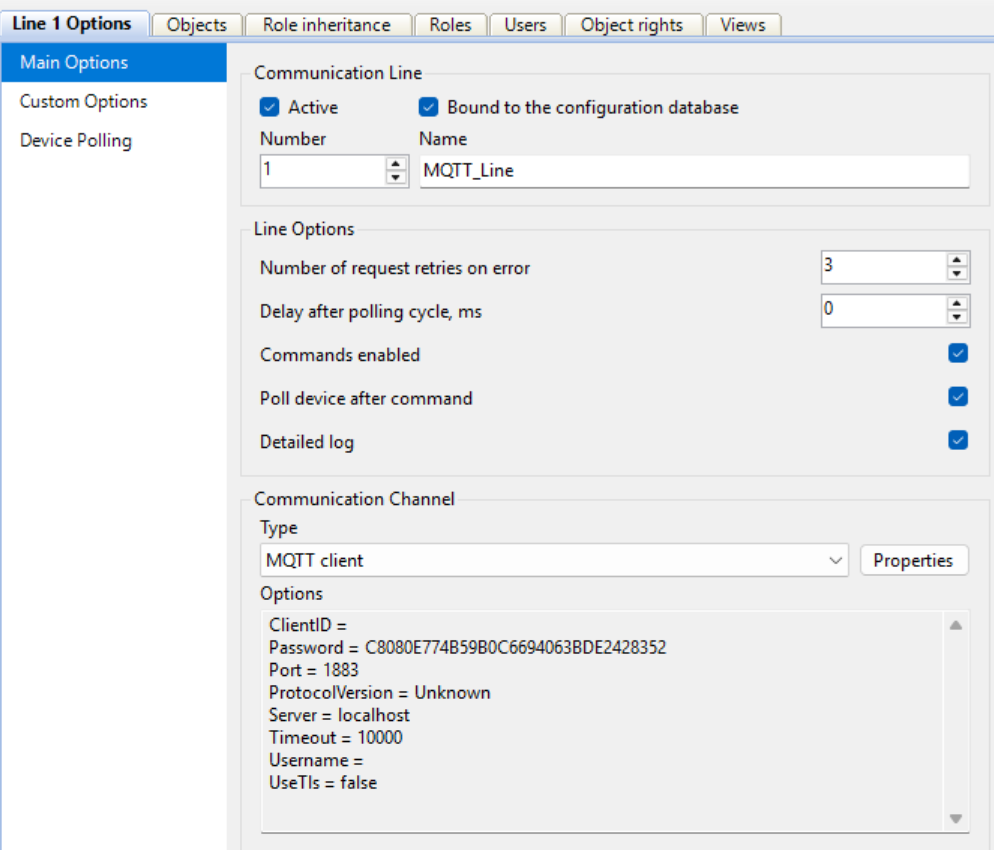
\includegraphics[width=0.45\linewidth]{images/comm_line_mqtt.png}
    \caption{\textit{Communication Line} en RapidScada}
\end{figure}
\subsubsection*{Configuració del dispositiu MQTT}

Un cop definida la línia de comunicació, el següent pas és crear un dispositiu associat a aquesta línia. Dins d'aquest dispositiu, cal configurar el \textbf{Driver}: \texttt{DrvMqttClient}. Aquest és l'encarregat de gestionar la comunicació MQTT dins de RapidSCADA.

\begin{figure}[H]
    \centering
    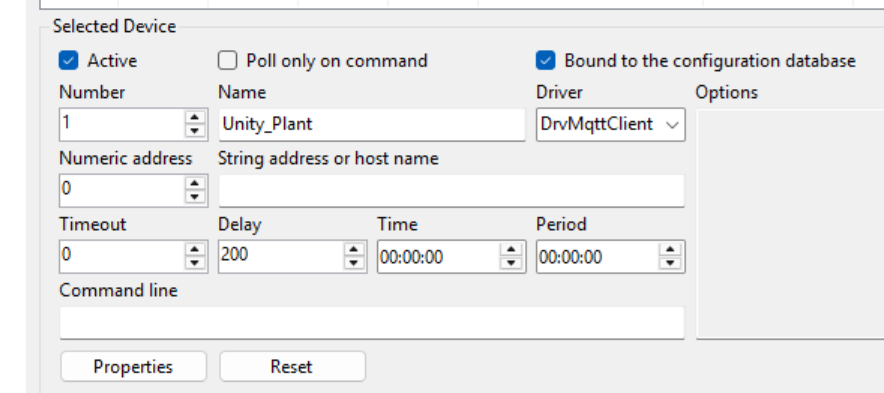
\includegraphics[width=0.5\linewidth]{images/device_mqtt.png}
    \caption{\textit{Device} en RapidScada}
\end{figure}

En aquesta etapa es defineixen dos elements fonamentals:

\paragraph{Subscripcions (\textit{Subscriptions})}:  Permeten especificar els \textit{topics} als quals RapidSCADA es subscriurà per rebre dades des de Unity. Per a cada subscripció es defineix:
\begin{itemize}
    \item El \textbf{topic MQTT}
    \item Un \textbf{identificador o tag}
    \item El tipus d'accés (normalment només lectura)
    \item Opcionalment, un codi en JavaScript per processar les dades rebudes
\end{itemize}

En aquest projecte, no s'ha utilitzat processament addicional, ja que cada variable es publica en un \textit{topic} independent, facilitant el seu tractament directe.

És important destacar que, tot i que una subscripció està pensada principalment per a la lectura de dades, en el context de Rapid SCADA el canal associat pot utilitzar-se tant com a \textit{input channel} com a \textit{output channel}. Això permet que un mateix \textit{topic} pugui servir tant per rebre com per enviar valors, depenent de la configuració del canal.

\paragraph{Comandes (\textit{Commands})}

Permeten definir els \textit{topics} als quals RapidSCADA enviarà informació. Aquests \textit{topics} corresponen a les ordres que controlen el comportament de la planta en Unity, com per exemple ordres manuals o canvis de mode de funcionament.

A diferència de les subscripcions, els \textit{topics} definits com a comandes tenen un comportament exclusivament d'escriptura, ja que només s'utilitzen per enviar dades des de Rapid SCADA cap a Unity. Aquest funcionament segueix la lògica pròpia del protocol MQTT: per rebre dades és necessari estar subscrit a un \textit{topic}, mentre que per enviar informació només cal publicar-hi missatges, sense necessitat de cap subscripció prèvia.

\begin{figure}[H]
\centering
\begin{minipage}{0.42\textwidth}
    \centering
    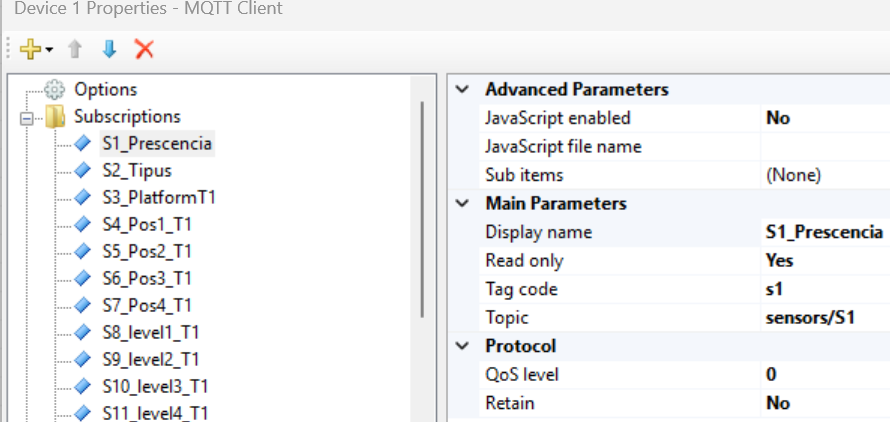
\includegraphics[width=\linewidth]{images/subscription.png}
\end{minipage}
\hfill
\begin{minipage}{0.52\textwidth}
    \centering
    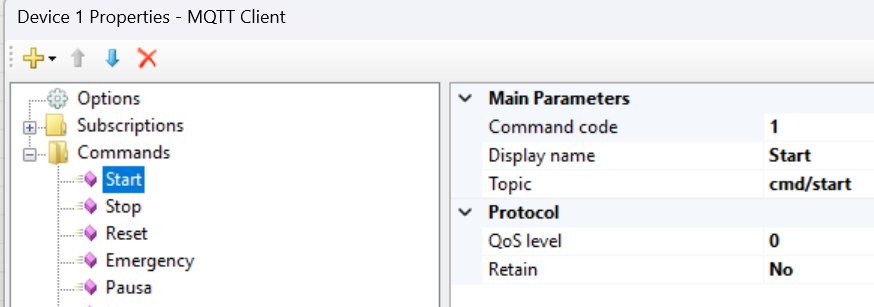
\includegraphics[width=\linewidth]{images/commands.png}
\end{minipage}
\caption{\textit{Subscriptions} i \textit{Commands} en RapidScada}
\end{figure}

\subsubsection*{Creació dels canals}

Una vegada configurat el dispositiu, és necessari crear els canals (\textit{channels}) \cite{rapidscada_channels} que representaran cadascuna de les variables dins del sistema SCADA i els quals actuan com a punt d'accés a les dades. Per a cada canal es defineix:
\begin{itemize}
    \item La línia de comunicació associada
    \item El dispositiu MQTT
    \item L'objecte (habitualment \textit{Enterprise} en cas de no haver creat cap objecte específic)
    \item El valor o índex del canal corresponent
\end{itemize}

\subsubsection*{Configuració avançada dels canals}

Finalment, tots els canals creats es poden visualitzar i configurar des de la base de dades de configuració, concretament a la taula \textit{Channels} dins de \textit{Primary Table}. En aquesta taula es poden ajustar diversos paràmetres:

\begin{itemize}
    \item Tipus d'accés (lectura o escriptura)
    \item Tipus de dada (per exemple: \textit{On-Off}, \textit{Yes-No})
    \item Nombre de decimals
    \item Altres propietats de visualització
\end{itemize}

Cal destacar que, en alguns casos, hauria estat útil treballar amb variables de tipus \textit{string}. No obstant això, no s'ha aconseguit visualitzar correctament aquest tipus de dades dins de RapidSCADA en el context del projecte.


\newpage
\section{Pantalles HMI amb Rapid SCADA}
\label{sec:hmi}
Continuant amb els conceptes de comunicació mitjançant MQTT i la integració amb Rapid SCADA descrits en l'apartat anterior, en aquesta secció es detalla com es dissenyen les pantalles HMI que permeten visualitzar i interactuar amb les variables del sistema.

L'objectiu principal d'aquestes pantalles és oferir una interfície clara i intuïtiva que permeti \textbf{visualitzar} l'estat del sistema en temps real, \textbf{interpretar} el comportament dels sensors i actuadors i \textbf{interactuar} amb el procés industrial simulat


\subsection{Estructura de les vistes en Rapid SCADA}

Per a la creació de pantalles, Rapid SCADA utilitza el mòdul \textit{Views} \cite{rapidscada_views}, des del qual es poden generar diferents tipus d'arxius visuals accessibles per l'usuari.

Inicialment, es va crear una vista de tipus \texttt{.tbl} anomenada \textit{System Overview}, amb l'objectiu de visualitzar totes les variables del sistema a través dels canals configurats. Aquesta vista permetia observar en temps real els valors dels tòpics MQTT, però presentava una limitació important: la manca d'una representació visual intuïtiva. Per aquest motiu, es van desenvolupar \textbf{tres pantalles HMI} orientades a millorar la visualització i el control del sistema.

Pel que fa a la navegació entre pantalles, aquesta es realitza exclusivament mitjançant el menú predefinit de Rapid SCADA (figura \ref{fig:menu_hmi}). L'eina no permet implementar una estructura de navegació interna personalitzada dins de les pròpies vistes, fet que limita la flexibilitat en el disseny de la interfície d'usuari.


\begin{figure}[H]
    \centering
    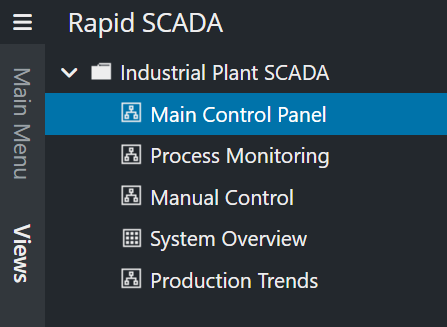
\includegraphics[width=0.32\linewidth]{images/menu_hmi.png}
    \caption{Menú de navegació entre pantalles en Rapid SCADA}
    \label{fig:menu_hmi}
\end{figure}



\subsection{Pantalla de visualització de sensors}

Aquesta pantalla (figura \ref{fig:pantalla_sensors}) està orientada exclusivament al monitoratge del sistema, sense capacitat d'interacció directa.Per al seu desenvolupament s'ha utilitzat el format \texttt{.sch} (\textit{ScadaSchemeEditor}), que permet incloure elements gràfics com textos, imatges i indicadors dinàmics.

\begin{figure}[H]
    \centering
    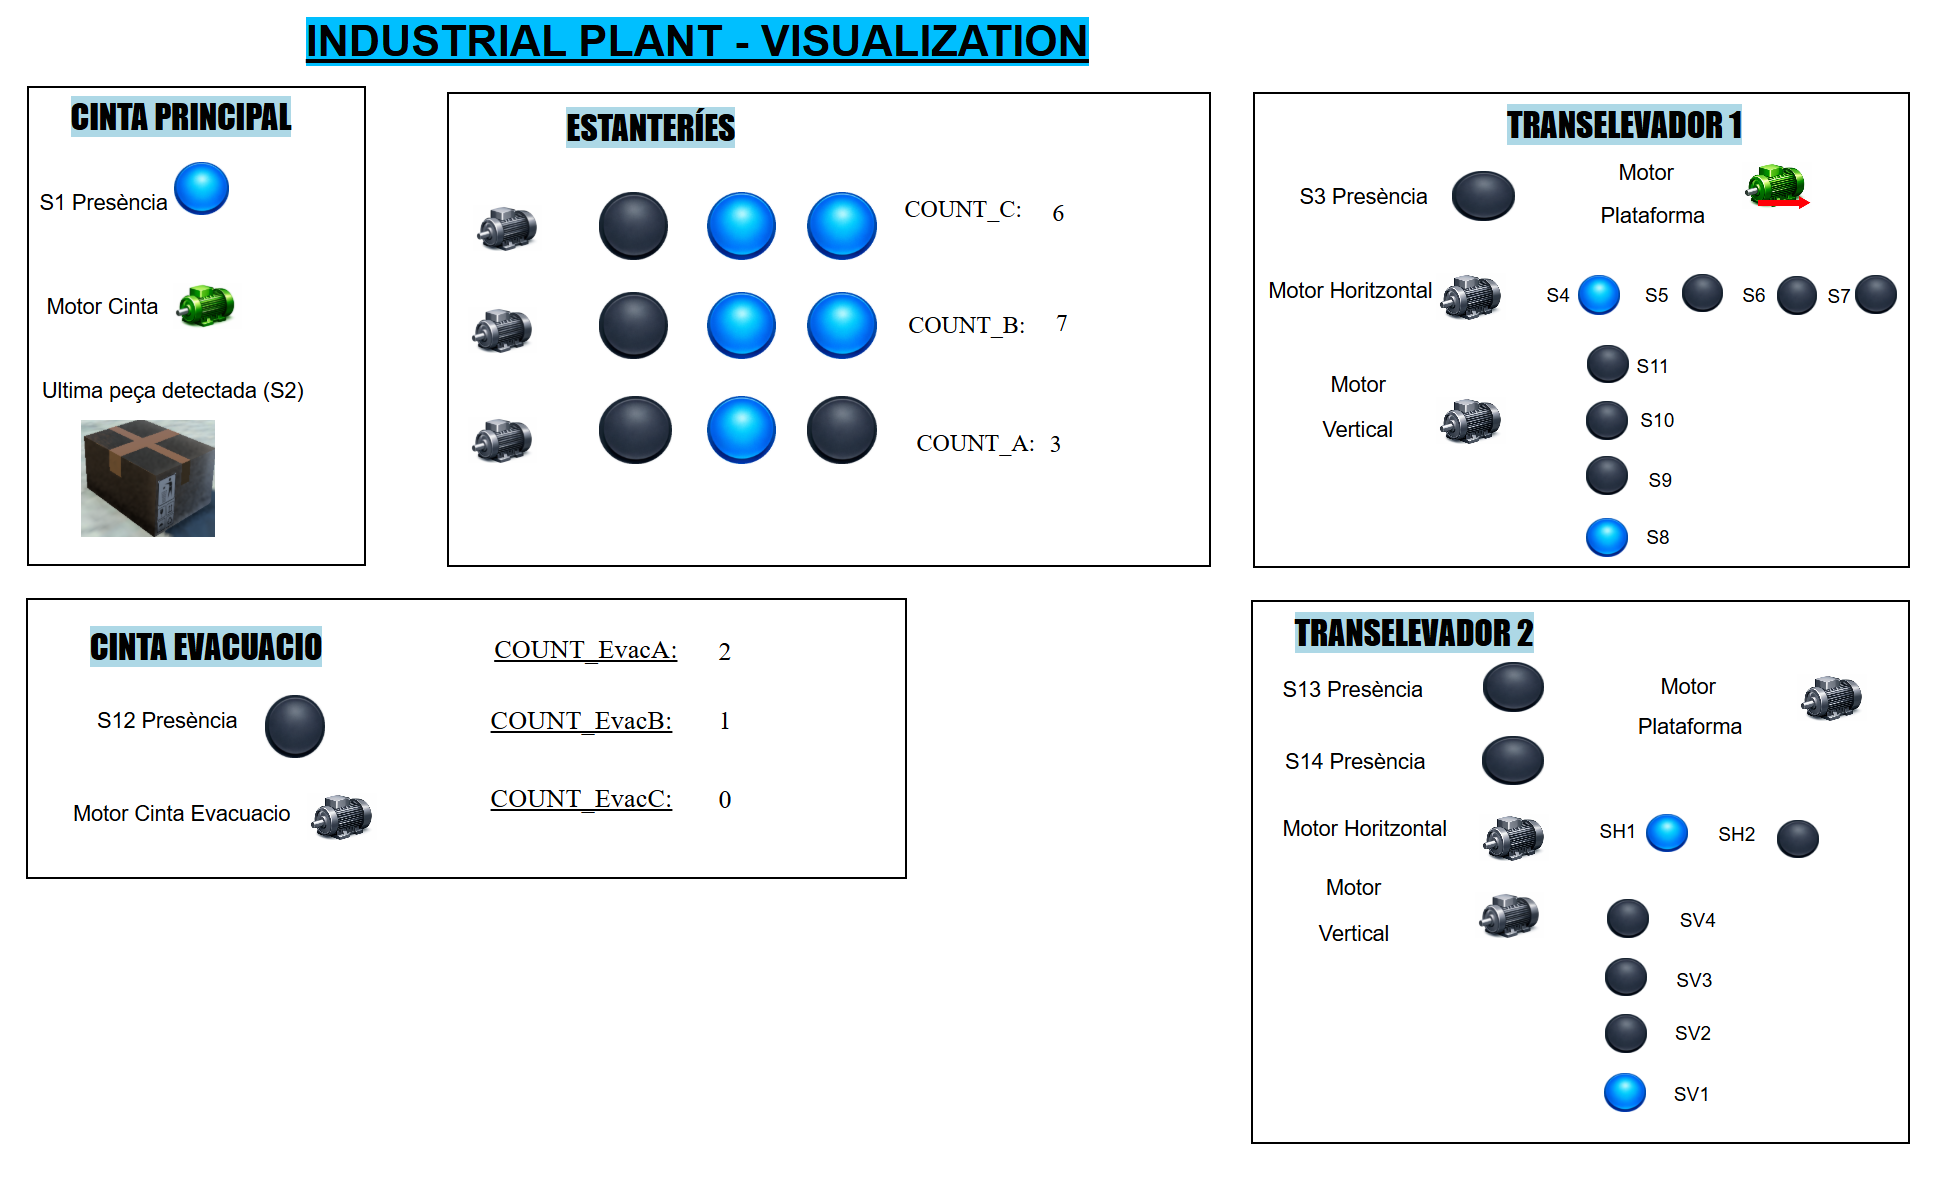
\includegraphics[width=0.9\linewidth]{images/pantalla_sensors.png}
    \caption{Pantalla de visualització de sensors}
    \label{fig:pantalla_sensors}
\end{figure}

%%\subsubsection{Funcionament general}

Les dades generades a Unity (com sensors de presència, posició o comptadors) són publicades mitjançant MQTT i rebudes a Rapid SCADA a través dels canals d'entrada. Aquesta pantalla permet visualitzar en temps real l'estat d'aquestes variables, facilitant la comprensió del comportament del sistema.

\subsubsection{Elements utilitzats}

\begin{itemize}
    \item \textbf{Static Text}: utilitzat per títols i etiquetes fixes.
    \item \textbf{Dynamic Text}: mostra valors en temps real associats a canals.
    \item \textbf{Dynamic Image}: element clau per representar visualment l'estat de sensors i actuadors.
\end{itemize}

Els \textit{Dynamic Text} s'associen a un canal d'entrada (\textit{input channel}), mostrant en tot moment el valor actual publicat al tòpic MQTT corresponent. Aquest element és útil per representar els comptadors dintre de les nostres pantalles, sabent el seu valor en temps real \cite{RapidScadaVideos}.  El component més rellevant és el \textit{Dynamic Image} , que permet canviar la imatge en funció del valor rebut:

\begin{itemize}
    \item Sensors binaris: dues imatges (0 = apagat, 1 = activat) (figura \ref{fig:sensor_estat})
    \item Motors: estat actiu/inactiu (figura \ref{fig:motor_estat1})
    \item Rodets: tres estats (stop, forward, reverse) (figura \ref{fig:motor_estat2})
    \item Sensor òptic: imatge segons el tipus de peça detectada, treta de la simulació realitzada en Unity. 
\end{itemize}

\subsubsection{Representació gràfica dels elements}

A continuació es mostren exemples representatius dels diferents tipus d'elements visuals utilitzats i una imatge de la vista general de la pantalla:

\begin{figure}[H]
    \centering
    
\includegraphics[width=0.1\linewidth]{images/sensor_off.png}
    
\includegraphics[width=0.1\linewidth]{images/sensor_on.png}
    \caption{Representació d'un sensor en estat apagat i activat}
    \label{fig:sensor_estat}
\end{figure}

\begin{figure}[H]
    \centering
    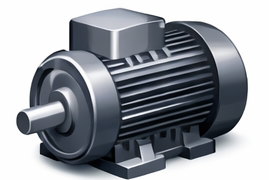
\includegraphics[width=0.1\linewidth]{images/motor_off.png}
    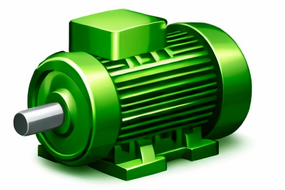
\includegraphics[width=0.1\linewidth]{images/motor_on.png}
    \caption{Representació d'un motor en estat inactiu i actiu}
    \label{fig:motor_estat1}
    \centering
    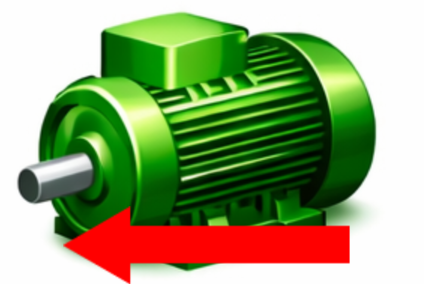
\includegraphics[width=0.1\linewidth]{images/motor_forward.png}
    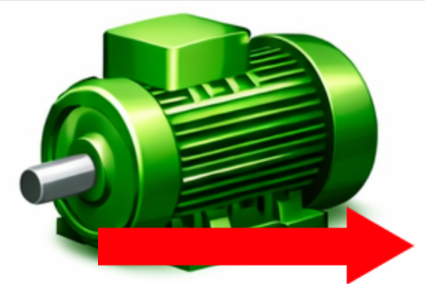
\includegraphics[width=0.1\linewidth]{images/motor_reverse.png}
    \caption{Estats dels rodets: endavant i enrere}
    \label{fig:motor_estat2}
\end{figure}

\subsection{Pantalla de control del procés}

La segona pantalla està orientada al control del sistema i permet enviar comandes als actuadors (figura \ref{fig:main_screen}).

\begin{figure}[H]
    \centering
    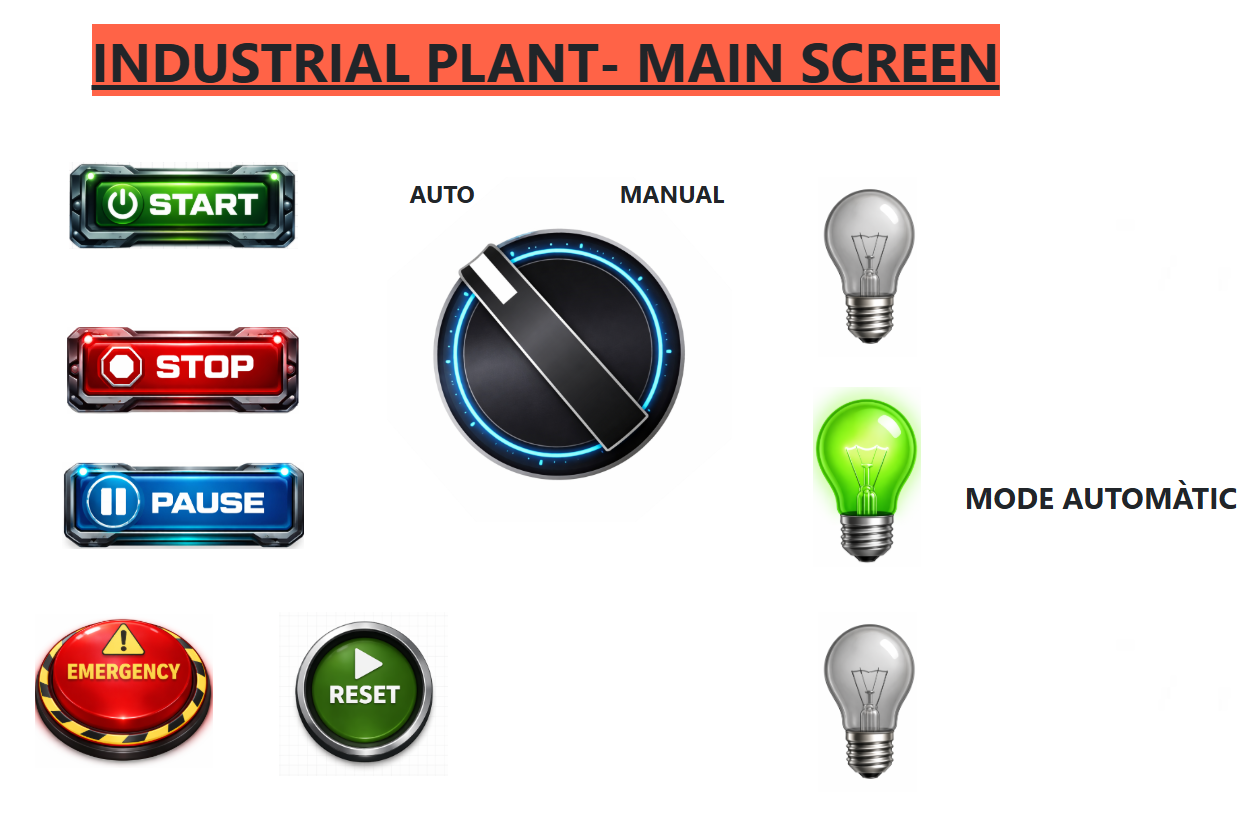
\includegraphics[width=0.75\linewidth]{images/MAIN_SCREEN.png}
    \caption{Pantalla de control del procés}
    \label{fig:main_screen}
\end{figure}


Per a la seva implementació s'ha utilitzat el tipus \textit{Mimic Diagram}, que requereix la instal·lació d'un plugin específic de Rapid SCADA.


A diferència del format \texttt{.sch}, el Mimic Diagram \cite{RapidScadaMimicVideo} permet enviar comandes directament als canals mitjançant la funcionalitat \textit{Send Command}, facilitant la interacció amb el sistema.Aquesta pantalla inclou:

\begin{itemize}
    \item Botons de \textbf{Start} i \textbf{Stop}
    \item Selector de mode (Manual / Automàtic / Neutre)
    \item Botó d'\textbf{Emergència}
    \item Botó de \textbf{Reset}
    \item Botó de \textbf{Pause} 
\end{itemize}

\subsubsection{Implementació dels elements interactius}
\subsubsection*{Selector de mode}

El selector de mode s'ha implementat mitjançant:
\begin{itemize}
    \item Un element visual amb \textit{input channel} (estat actual)
    \item Tres zones invisibles superposades que envien comandes segons la posició seleccionada
\end{itemize}

Aquest mètode permet simular un selector físic dins de l'entorn HMI (figura \ref{fig:selector_mode}). La imatge del selector està vinculada a un \textit{input channel}, de manera que mostra en tot moment l'últim valor assignat a aquest element.

\begin{figure}[H]
\centering
\begin{minipage}{0.32\textwidth}
    \centering
    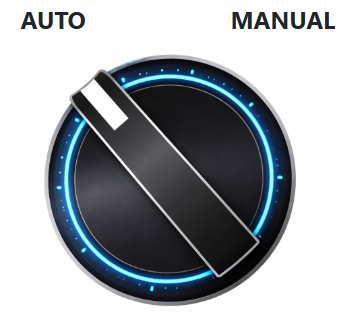
\includegraphics[width=\linewidth]{images/selector_0.png}
    \caption*{Mode automàtic}
\end{minipage}
\begin{minipage}{0.32\textwidth}
    \centering
    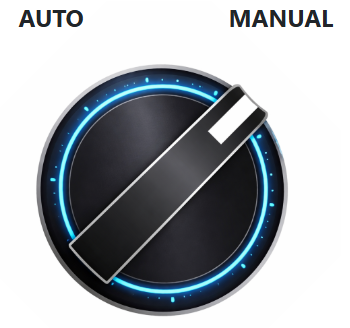
\includegraphics[width=\linewidth]{images/selector_1.png}
    \caption*{Mode manual}
\end{minipage}
\begin{minipage}{0.32\textwidth}
    \centering
    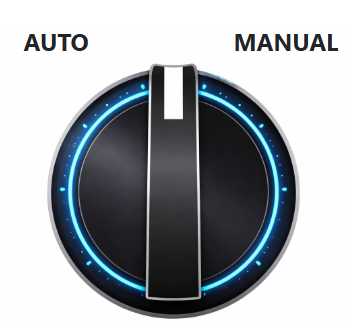
\includegraphics[width=\linewidth]{images/selector_-1.png}
    \caption*{Mode emergència}
\end{minipage}
\caption{Posicions del selector de mode}
\label{fig:selector_mode}
\end{figure}

\subsubsection*{Botons de control}

Durant la implementació de la pantalla de control, es va observar que alguns botons (com Start, Stop o Emergència) presentaven un comportament unidireccional, és a dir, permetien enviar un valor però no gestionar correctament el canvi d'estat.

Per solucionar aquesta limitació \cite{RapidScadaVideos}, es va implementar una tècnica basada en l'ús de \textbf{toggles invisibles} superposats als elements de control. Cada botó es va associar a un canal configurat com a \textit{input} i \textit{output}, permetent conèixer en tot moment el seu estat.

El funcionament consisteix en un botó visual amb una imatge dinàmica vinculada al canal, sobre el qual es col·loca un toggle invisible que, en ser activat, envia el valor contrari a l'estat actual. D'aquesta manera, s'aconsegueix un comportament bidireccional coherent amb la representació gràfica del botó.

Tot i això, aquesta solució presenta una limitació respecte als sistemes industrials reals. Habitualment, botons com \textbf{Start} i \textbf{Stop} són de tipus momentani,és a dir, només estan actius mentre es mantenen premuts, retornant automàticament al seu estat inicial, mentre que altres com el d'\textbf{Emergència} són biestables. En el Mimic Diagram no s'ha pogut reproduir aquest comportament de forma directa, de manera que tots els botons s'han implementat com a biestables.

Aquesta simplificació pot generar situacions no desitjades, com l'activació simultània de \textbf{Start} i \textbf{Stop}, fet que s'ha resolt a nivell de control mitjançant la lògica definida en el GRAFCET (Figura \ref{fig:botons_control}).


\begin{figure}[H]
\centering
\begin{minipage}{0.38\textwidth}
    \centering
    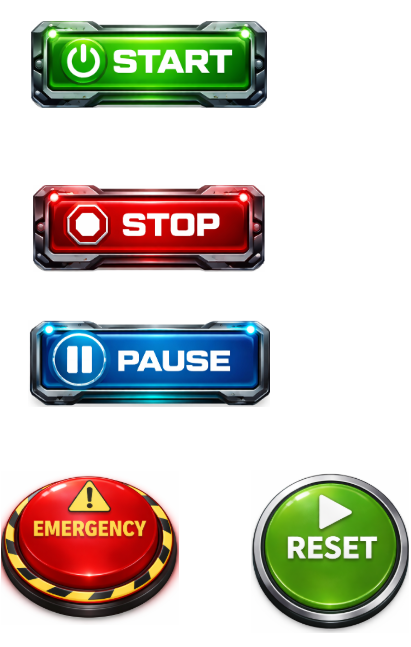
\includegraphics[width=\linewidth]{images/botons_no.png}
    \caption*{Botons en estat inactiu}
\end{minipage}
\hfill
\begin{minipage}{0.40\textwidth}
    \centering
    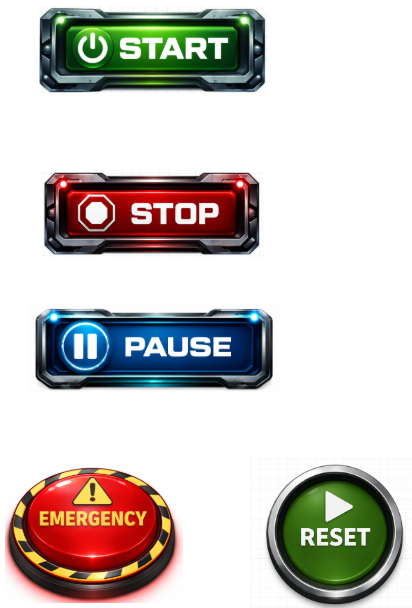
\includegraphics[width=\linewidth]{images/botons_si.png}
    \caption*{Botons en estat actiu}
\end{minipage}
\caption{Comparativa dels estats dels botons de control}
\label{fig:botons_control}
\end{figure}


\subsubsection*{Indicadors visuals}

La pantalla també incorpora indicadors lluminosos que mostren el mode específic en el que es troba el sistema de la planta industrial (emergència, manual o automàtic, figura \ref{fig:indicadors_mode}), acompanyat de 3 textos que apareixen o desapareixen en concordancia amb el mode actiu. 

\begin{figure}[H]
\centering
\begin{minipage}{0.32\textwidth}
    \centering
    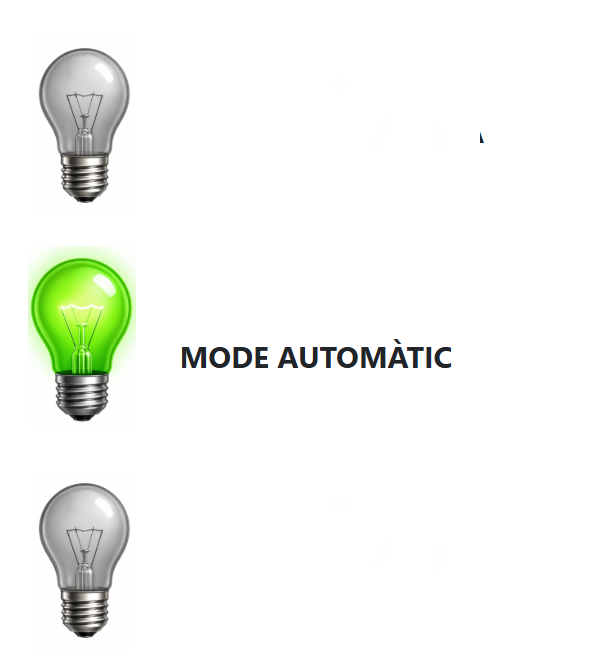
\includegraphics[width=\linewidth]{images/light_auto.png}
    \caption*{Mode automàtic}
\end{minipage}
\begin{minipage}{0.32\textwidth}
    \centering
    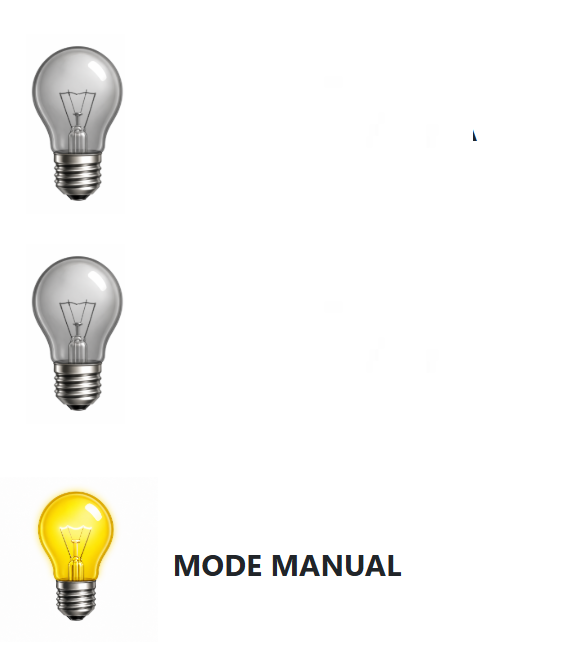
\includegraphics[width=\linewidth]{images/light_manu.png}
    \caption*{Mode manual}
\end{minipage}
\begin{minipage}{0.32\textwidth}
    \centering
    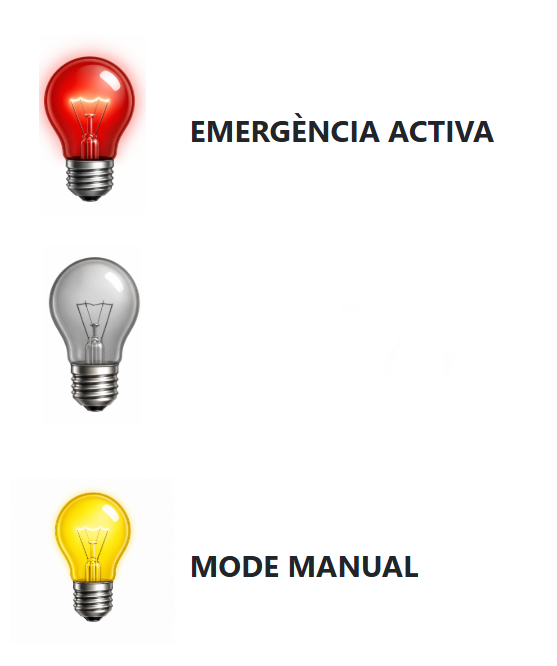
\includegraphics[width=\linewidth]{images/light_emerg.png}
    \caption*{Mode emergència}
\end{minipage}
\caption{Diferents estats dels indicadors de mode}
\label{fig:indicadors_mode}
\end{figure}



\subsection{Pantalla de mode manual}

La tercera pantalla està destinada al control manual dels actuadors del sistema (Figura \ref{fig:manual_screen}). També s'ha implementat mitjançant \textit{Mimic Diagram}, degut a la necessitat d'enviar comandes directes. A diferència de les altres pantalles, aquesta no utilitza canals d'entrada, ja que el seu objectiu és únicament enviar comandes al sistema.


\begin{figure}[H]
    \centering
    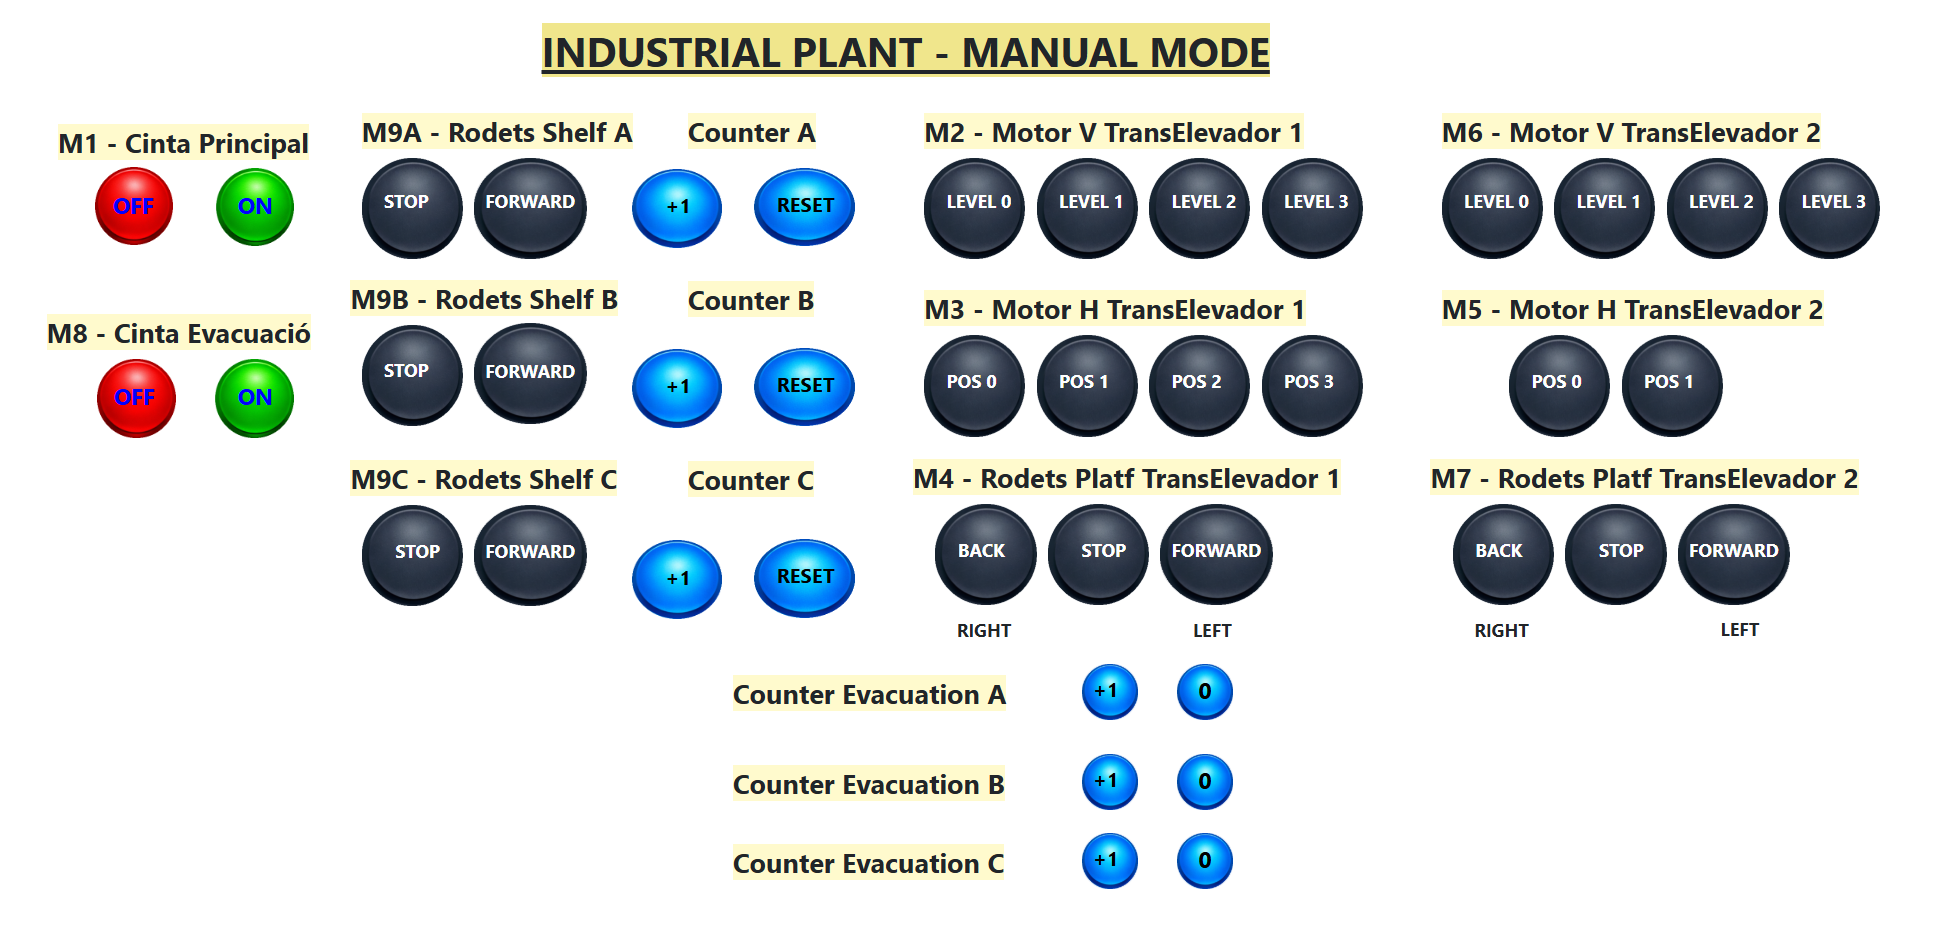
\includegraphics[width=0.9\linewidth]{images/manual_screen.png}
    \caption{Pantalla de control manual}
    \label{fig:manual_screen}
\end{figure}

Els elements disponibles són:

\begin{itemize}
    \item Cintes transportadores: botons de start/stop que permeten activar o aturar el moviment de la cinta. Quan es prem un botó, s'envia un valor binari (0 o 1) al canal corresponent, que Unity interpreta per iniciar o detenir el desplaçament de les peces.

    \item Rodets de plataformes: tres botons associats a cada sistema de rodets:
    \begin{itemize}
        \item Endavant (valor positiu, habitualment 1)
        \item Enrere (valor negatiu, habitualment -1)
        \item Aturat (valor 0)
    \end{itemize}
    \item Transelevadors: el seu control es basa en l'enviament de \textbf{posicions discretes} en lloc de moviments continus.   
    Cada transelevador disposa de dos graus de llibertat:
    
    \begin{itemize}
        \item \textbf{Moviment horitzontal:} cada botó envia un valor enter que representa la posició objectiu al llarg dels carrils (per exemple, entre 1 i 4 segons el nombre de posicions disponibles).
        \item \textbf{Moviment vertical:} de manera anàloga, s'envien valors discrets que indiquen el nivell d'alçada desitjat.
    \end{itemize}

Aquests valors són interpretats a Unity com a consignes de posició, encarregant-se el sistema de moure el transelevador fins a la ubicació indicada.

    \item Comptadors de producció i evacuació: botons que permeten incrementar manualment el valor dels comptadors o reinicialitzar-los a zero.
\end{itemize}



\subsection{Pantalla de gràfics i taula general}

Amb l'objectiu de millorar la visualització i anàlisi de les dades del sistema, s'han incorporat dues noves pantalles: una taula general i una pantalla de gràfics.

\subsubsection{Taula general de dades}

La taula general s'ha implementat mitjançant una vista de tipus \texttt{.tbl}, que permet visualitzar tots els canals configurats dins del sistema. Aquesta vista presenta les següents característiques:
\begin{itemize}
    \item Visualització en temps real dels canals d'entrada (\textit{input channels})
    \item Possibilitat d'enviar comandes als canals de sortida (\textit{output channels})
    \item Accés directe a les dades històriques
\end{itemize}

\subsubsection{Visualització de gràfics amb Chart Pro}

Per a la representació gràfica de dades, s'ha utilitzat el plugin \textbf{Chart Pro} \cite{rapidscada_chart_pro}, que amplia les funcionalitats del sistema base (Figura \ref{fig:tabla_grafico}). Les millores principals que aporta són:
\begin{itemize}
    \item Visualització de múltiples canals en un mateix gràfic
    \item Comparació simultània de variables
    \item Exportació de gràfics i dades en formats com PDF o PNG
\end{itemize}

A diferència del sistema base, que només permet visualitzar un canal per gràfic, aquest plugin facilita una anàlisi més completa del comportament del sistema.


\begin{figure}[H]
\centering
\begin{minipage}{0.48\textwidth}
    \centering
    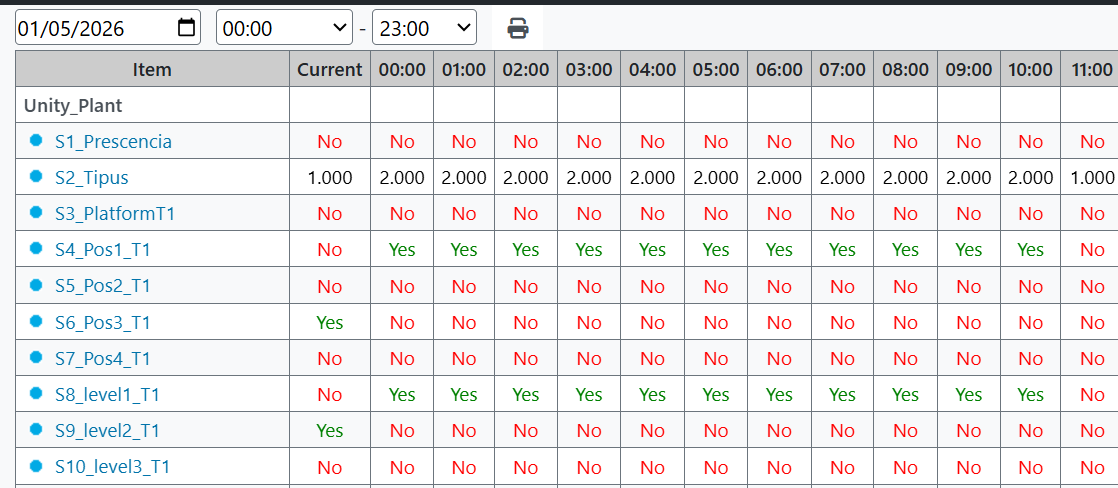
\includegraphics[width=\linewidth]{images/tabla_general.png}
    \caption*{Vista parcial de la taula de dades}
\end{minipage}
\hfill
\begin{minipage}{0.48\textwidth}
    \centering
    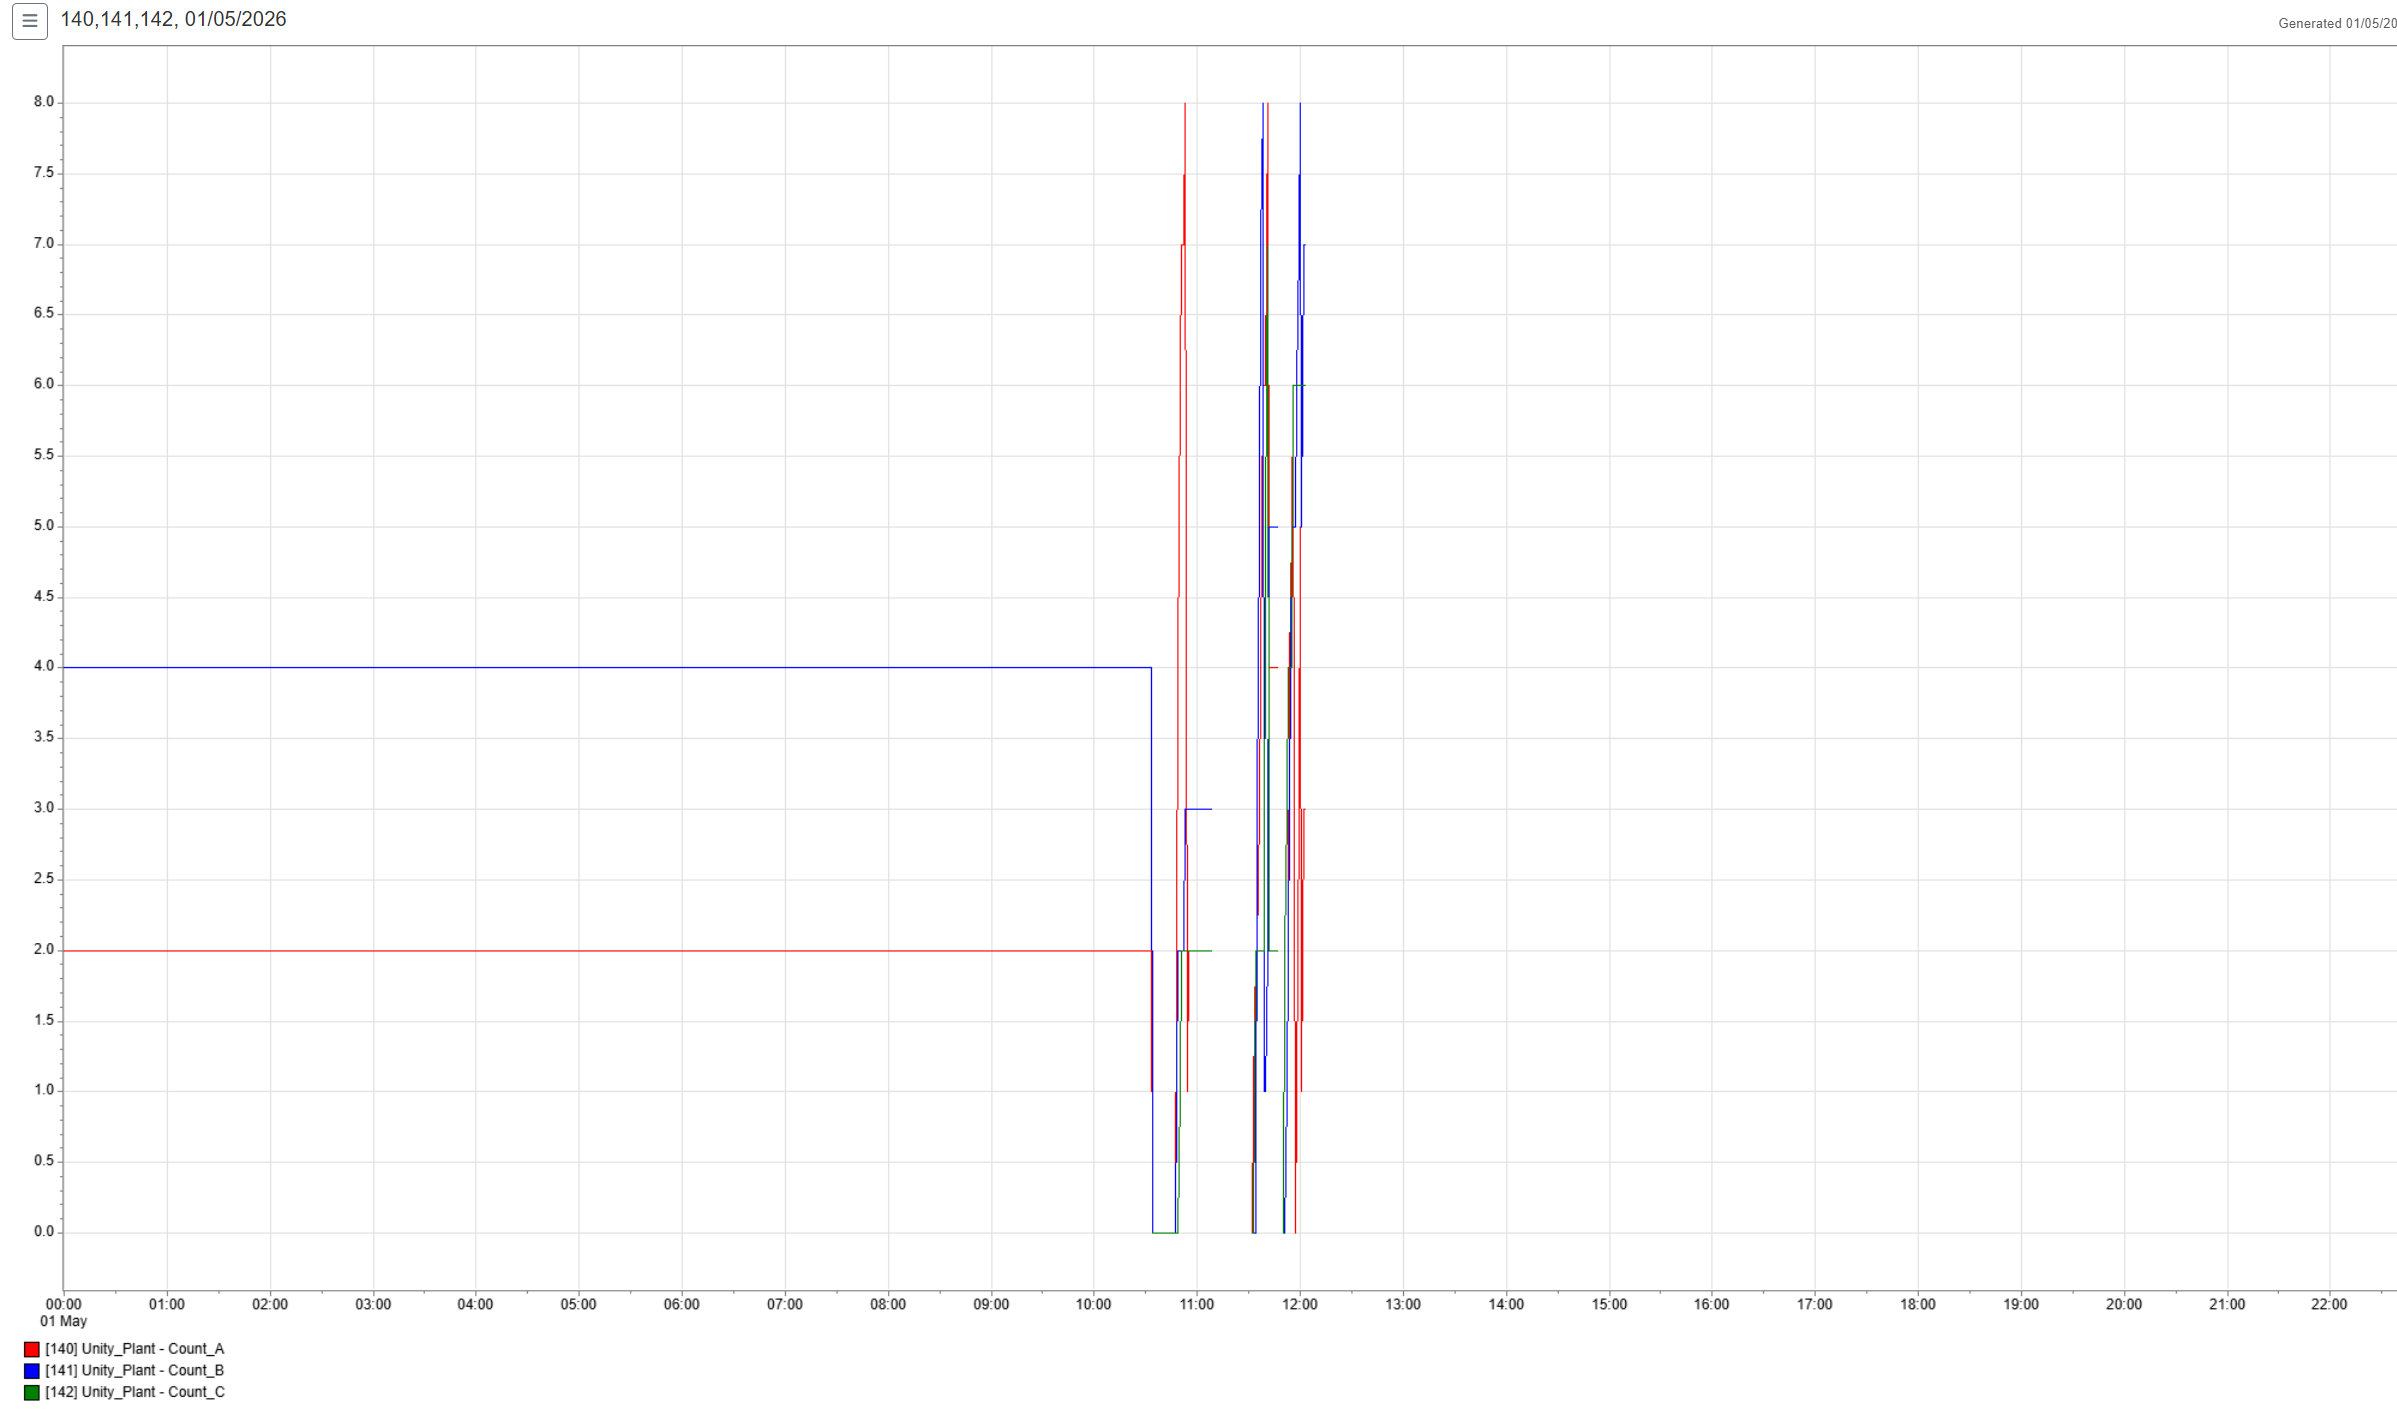
\includegraphics[width=\linewidth]{images/grafico_tabla.png}
    \caption*{Gràfic generat a partir de  les variables dels comptadors d'evacuació}
\end{minipage}
\caption{Relació entre la visualització tabular i la representació gràfica de dades}
\label{fig:tabla_grafico}
\end{figure}


La vista en format taula permet accedir directament als valors de les variables, mentre que la selecció d'un canal concret facilita la generació de gràfics per a l'anàlisi de la seva evolució temporal.

\subsubsection{Integració de gràfics en esquemes}

Addicionalment, s'ha creat una pantalla de tipus \texttt{.sch} utilitzant el plugin \textit{Extra Scheme Editor}, que permet integrar gràfics directament dins dels esquemes visuals. En aquest cas, s'ha implementat un gràfic (Figura \ref{fig:grafico_esquema}) que mostra les variables de comptador d'evacuació (EvacA, EvacB i EvacC), amb l'objectiu de comparar el rendiment del sistema.

Cal destacar que els gràfics integrats en fitxers \texttt{.sch} presenten certes limitacions en comparació amb els gràfics generats des de les vistes de tipus \texttt{.tbl} els quals, en seleccionar una variable, ofereixen funcionalitats més avançades, com:
\begin{itemize}
    \item Selecció d'intervals de temps
    \item Visualització detallada de l'evolució de la variable
    \item Major capacitat d'anàlisi de dades
\end{itemize}

Per tant, els gràfics en esquemes són útils per a una visualització integrada i immediata, mentre que les vistes \texttt{.tbl} resulten més adequades per a l'anàlisi detallada del sistema.

Cal destacar també que la correcta configuració de Chart Pro és necessària per visualitzar múltiples canals. En cas contrari, només es mostrarà un únic canal. A més, aquest plugin requereix una llicència (trial o permanent). De la mateixa manera passa amb el \textit{ExtraSchemeEditor}, que és necessari per veure el gràfic en aquesta mateixa pantalla, sinó l'única manera de visualitzar els gràfics és a través de la taula.


\begin{figure}[H]
    \centering
    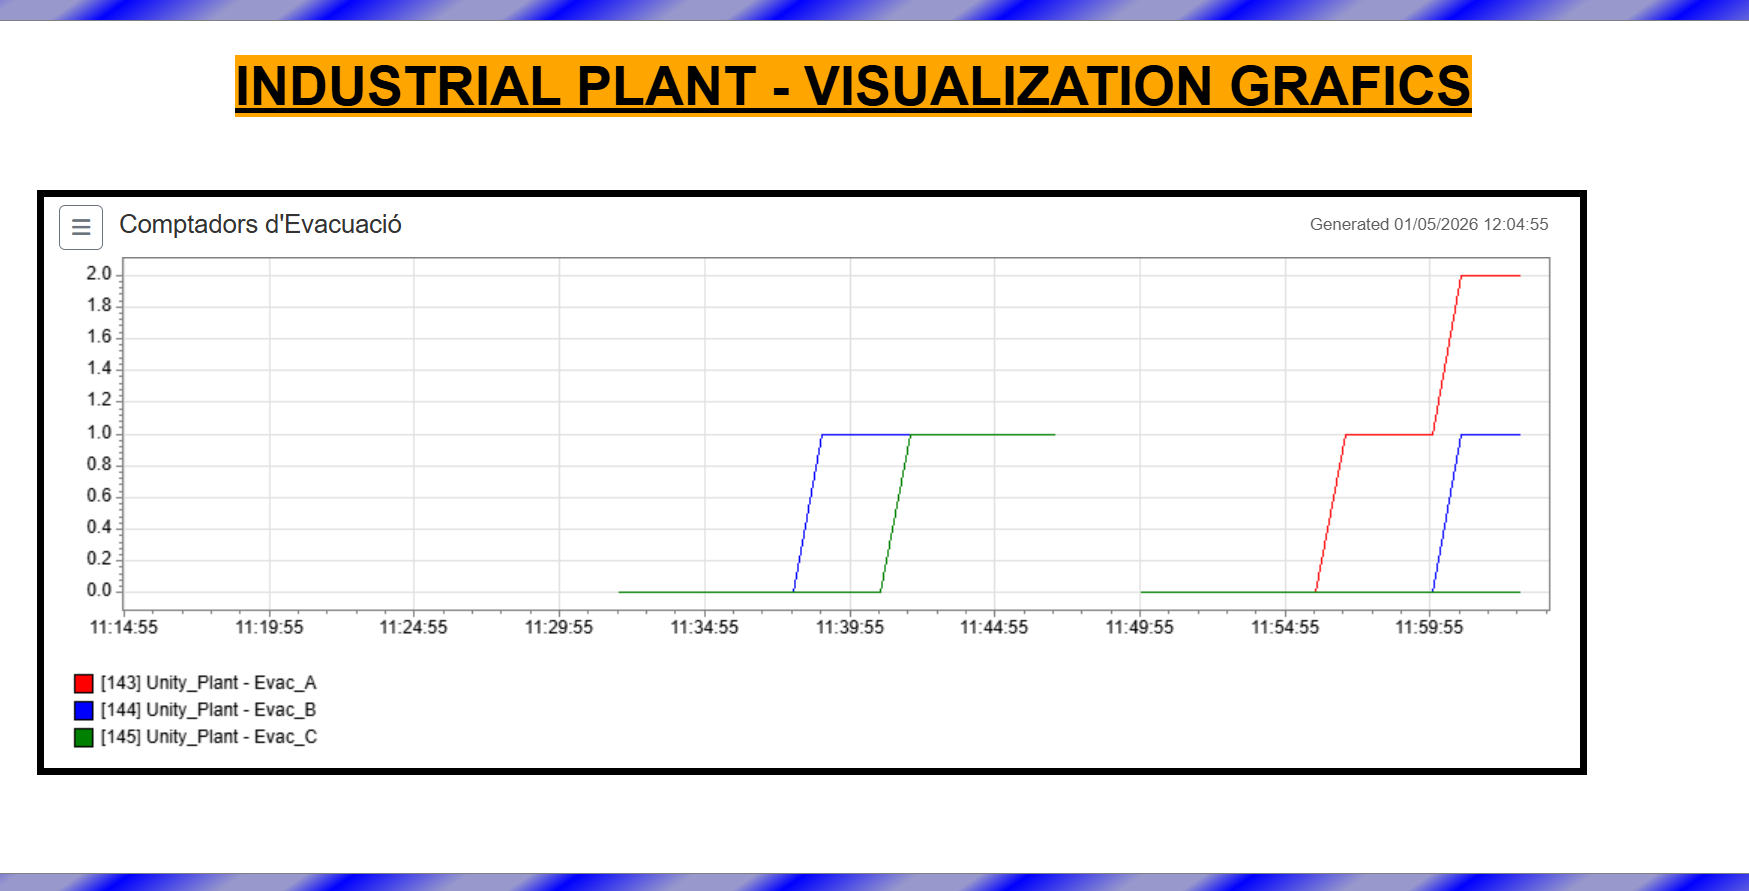
\includegraphics[width=0.8\linewidth]{images/grafico_esquema.png}
    \caption{Gràfic integrat dins d'un esquema utilitzant Extra Scheme Editor}
    \label{fig:grafico_esquema}
\end{figure}

\subsection{Configuració d'usuaris i control d'accés}

Per tal de gestionar correctament l'accés a les diferents funcionalitats del sistema, s'ha implementat un sistema de control basat en rols i permisos (Figura \ref{fig:objects_scada}). Primer de tot, s'han creat tres rols principals \cite{rapidscada_user_management}:  
\begin{itemize}
    \item \textbf{Supervisor}: accés complet al sistema
    \item \textbf{Operator}: accés parcial amb capacitat de control limitada
    \item \textbf{User}: accés únicament de visualització
\end{itemize}

\begin{figure}[H]
    \centering
    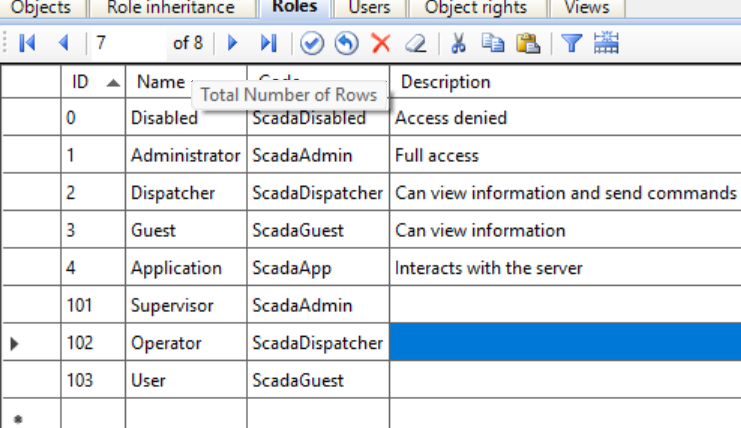
\includegraphics[width=0.5\linewidth]{images/rols_scada.png}
    \caption{Rols en RapidScada}
    \label{fig:rols_scada}
\end{figure}

Seguidament, les pantalles del sistema s'han organitzat en diferents categories amb l'objectiu de facilitar la gestió dels permisos d'accés mitjançant els \textit{Object rights} de Rapid SCADA (Figura \ref{fig:objects_scada}):

\begin{itemize}
    \item \textbf{Mode}: inclou les vistes generals del sistema (Vista\_Planta.tbl i MainScreen.mim)
    \item \textbf{Manual}: pantalla de control manual dels actuadors (ModeManual.mim)
    \item \textbf{Gràfics}: visualització de dades històriques (Grafics.sch)
    \item \textbf{Visualització}: pantalla de visualització de sensors, motors i comptadors (Visualization.sch)
\end{itemize}


Aquests grups permeten assignar permisos de forma estructurada mitjançant la configuració de \textit{Object rights}. Com a detall, indicar que els canals també tenen la opció de ser assignats a diferents categories, i si volem que poguin ser accesibles per un rols concrets, és necessari també assignar la categoria correctament.

\begin{figure}[H]
\centering
\begin{minipage}{0.5\textwidth}
    \centering
    \includegraphics[width=\linewidth]{images/objects_scada.png}
    \caption*{Creació objectes}
\end{minipage}
\hfill
\begin{minipage}{0.7\textwidth}
    \centering
    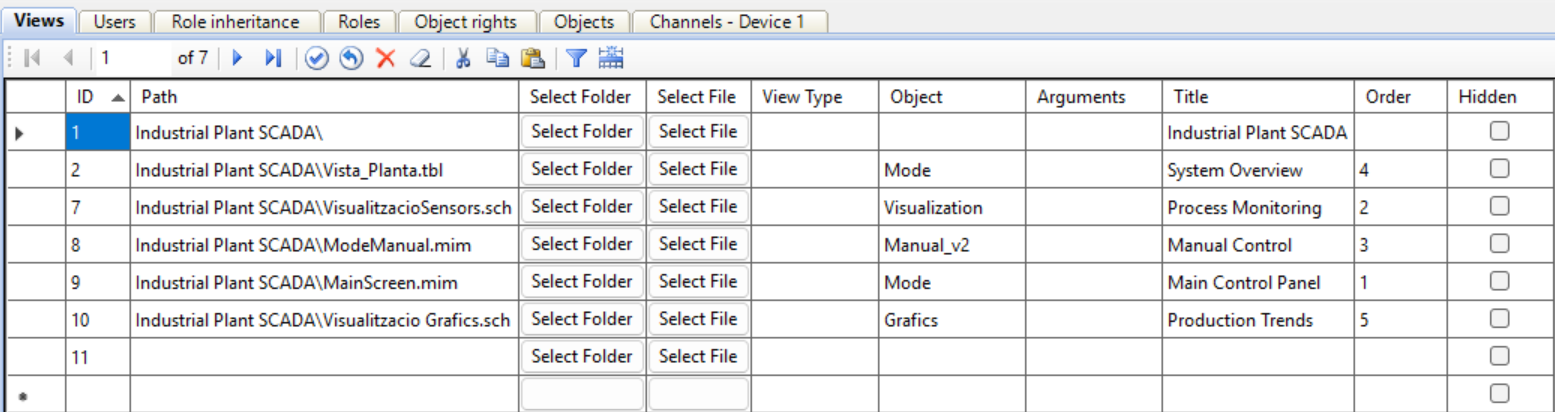
\includegraphics[width=\linewidth]{images/views_scada.png}
    \caption*{Assignació objectes}
\end{minipage}
\caption{Taules referents a objectes en RapidScada}
\label{fig:objects_scada}
\end{figure}
\subsubsection{Assignació de permisos}

Els permisos s'han distribuït de la següent manera (Figura \ref{fig:objectsrights_scada}):
\begin{itemize}
    \item \textbf{Supervisor}: accés complet a totes les pantalles i funcionalitats, amb permisos de \textit{View} i \textit{Control} en tots els casos.

    \item \textbf{Operator}: accés a la majoria de pantalles amb permisos de visualització en tots els modes, però amb capacitat de control restringida únicament a la pantalla de mode manual. Per aconsegui això, és necessari que tots els canals associats a la pantala de control manual, tinguin assignats la categoria \textbf{Manual}, així tant el supervisor com l'operador tenen accés a aquestes funcionalitats.

    \item \textbf{User}: accés limitat exclusivament a la visualització de dades, sense capacitat d'interacció amb el sistema.
\end{itemize}
\begin{figure}[H]
    \centering
    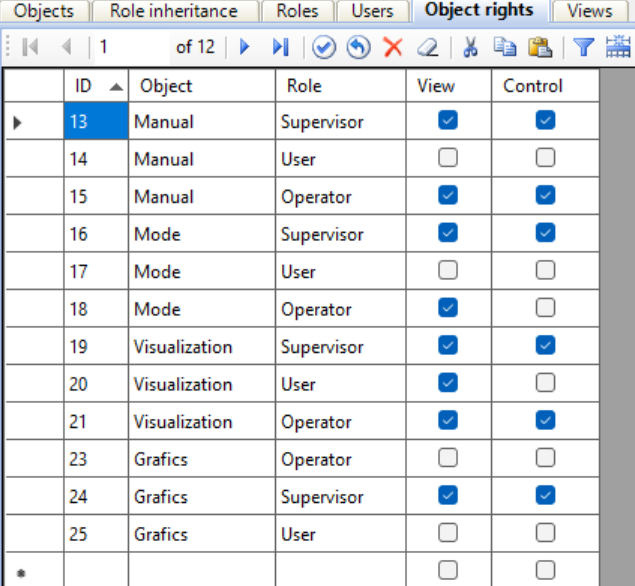
\includegraphics[width=0.32\linewidth]{images/objectsrights_scada.png}
    \caption{Assignació objectes a rols en RapidScada}
    \label{fig:objectsrights_scada}
\end{figure}

\subsubsection{Creació d'usuaris}

S'han creat diferents usuaris associats als rols definits, cadascun amb les seves credencials d'accés. Per tal de simplificar la gestió, els noms dels usuaris coincideixen amb els rols corresponents.

La configuració de les credencials es realitza des de l'eina d'administració de Rapid SCADA, on es poden definir les contrasenyes i assignar els rols de manera individual.

Cal destacar que Rapid SCADA inclou usuaris i rols predefinits (com l'usuari \textit{Admin}), que també poden ser utilitzats dins del sistema. En aquells casos en què no es defineixen explícitament permisos de \textit{View} o \textit{Control}, el comportament per defecte vindrà determinat per la configuració interna del sistema \ref{sec:scada_users}.



\newpage
\section{Possibles millores i línies futures}

Tot i que el sistema desenvolupat compleix els objectius plantejats, existeixen diverses línies de millora que permetrien augmentar el seu realisme, escalabilitat i aproximació a entorns industrials reals.

En primer lloc, una millora significativa seria la substitució del protocol MQTT per una arquitectura basada en \textbf{OPC UA}, on Unity actuaria com a servidor i Rapid SCADA com a client. Aquesta aproximació permetria una comunicació més estandarditzada i pròpia de la indústria, així com una millor gestió de les dades i menor càrrega en determinats escenaris.

En segon lloc, es planteja la migració del sistema a un entorn amb \textbf{accés remot mitjançant IP pública}, permetent visualitzar la Webstation de Rapid SCADA des de fora de la màquina local. Aquesta millora facilitaria l'accés remot, la demostració del sistema i la seva escalabilitat en entorns distribuïts. Aquest fet també ajudaria a que el broker MQTT que s'ha fet servir sigués també públic pero conrolat personalment, provocant que no fes falta al usuari configurar el broker MQTT en el seu dispositiu, ja que el sistema estaria configurat per connectar-se automàticament al broker públic. En cas d'aplicar aquesta millora, seria necessari implementar mesures de seguretat adequades, com ara l'ús de connexions segures (TLS) i autenticació per garantir la protecció de les dades i el control d'accés al sistema.

A nivell funcional, es proposa augmentar la complexitat del sistema mitjançant la incorporació de nous \textbf{modes de funcionament} i una gestió més avançada de situacions d'\textbf{emergència i avaria}. Això inclouria la simulació de fallades addicionals i la implementació de mecanismes de protecció dins de Unity, millorant el realisme del model.

També es planteja com a possible millora l'augment del realisme visual i funcional de l'entorn desenvolupat en Unity. Això inclouria la incorporació de \textbf{sons ambientals industrials}, efectes d'àudio associats al funcionament de cintes transportadores, motors o alarmes, així com millores gràfiques relacionades amb il·luminació, materials i animacions. De la mateixa manera, seria interessant implementar un \textbf{operari virtual} o personatge interactiu capaç de desplaçar-se per la planta industrial i interactuar amb determinats elements del sistema.

Pel que fa a la visualització i explotació de dades, seria convenient aprofundir en l'ús de \textbf{plugins i mòduls de Rapid SCADA}, així com integrar \textbf{bases de dades externes} (com PostgreSQL o InfluxDB). Aquesta integració és especialment rellevant, ja que el sistema intern de Rapid SCADA es basa en fitxers \texttt{.dat} i no permet la realització de consultes SQL directes, limitant l'anàlisi avançada de la informació. La qüestió important dels plugins que l'óptim seria tindre una clau permanent d'aquests plugins que permetés utilitzar-ho amb tota la llibertat possible, sense necessitat de demanar una \textit{Trial Key} cada dia.

Finalment, com a línia de futur amb alt valor afegit, es proposa la incorporació de tecnologies de \textbf{realitat virtual (VR)} dins de Unity, permetent una visualització immersiva de la planta industrial i millorant tant la interacció com el realisme del sistema.
\newpage

\section{Conclusió}

Com a conclusió d'aquest Treball de Fi de Grau, es pot afirmar que els objectius plantejats inicialment s'han assolit de manera satisfactòria. S'ha aconseguit dissenyar i implementar un sistema capaç d'integrar una plataforma SCADA de codi obert amb un entorn de visualització 3D en temps real aplicat a una planta industrial simulada, permetent així supervisar i controlar diferents processos industrials dins d'un entorn virtual interactiu.

Pel que fa a Rapid SCADA, el treball ha permès analitzar el funcionament i les possibilitats d'un sistema SCADA basat en programari lliure. Durant el desenvolupament s'ha comprovat que Rapid SCADA ofereix funcionalitats molt adequades per a tasques de supervisió i control industrial bàsic, permetent monitoritzar variables, visualitzar dades en temps real i establir comunicacions amb dispositius externs mitjançant protocols industrials habituals com MQTT, Modbus o OPC UA. A més, el fet de tractar-se d'un programari gratuït i relativament senzill de configurar el converteix en una eina molt interessant per a entorns educatius o petits projectes d'automatització.

No obstant això, també s'han identificat algunes limitacions. La interfície gràfica proporcionada per defecte és bastant simple i ofereix poques opcions de personalització i de navegació entre les diferents pantalles en comparació amb altres plataformes SCADA comercials. Per aconseguir interfícies més modernes o funcionals és necessari utilitzar plugins externs, molts dels quals són de pagament o disposen de versions de prova limitades. 

Respecte a Unity, el desenvolupament del projecte ha permès comprovar el gran potencial que ofereix aquest motor gràfic més enllà de l'àmbit dels videojocs. Tot i no haver treballat prèviament amb aquesta eina, la seva flexibilitat ha facilitat la creació d'una planta industrial virtual amb sensors, actuadors, sistemes de transport, transelevadors i diferents modes de funcionament. 

Pel que fa a la comunicació entre plataformes, la implementació mitjançant MQTT ha resultat especialment adequada gràcies a la seva simplicitat, flexibilitat i facilitat d'integració tant amb Rapid SCADA com amb Unity. Aquesta arquitectura ha permès establir una comunicació bidireccional en temps real entre el sistema SCADA i la simulació tridimensional de manera estable i escalable.

Finalment, en relació amb les possibilitats educatives i tècniques del projecte, es considera que la integració desenvolupada té un gran potencial com a eina d'aprenentatge dins de l'àmbit de l'automatització industrial i la indústria 4.0. La combinació d'un sistema SCADA amb un entorn virtual interactiu permet entendre de manera més visual i pràctica conceptes relacionats amb sensors, actuadors, comunicacions industrials i lògica de control.

Tot i això, en entorns industrials reals o en aplicacions de major complexitat, probablement seria convenient valorar l'ús de plataformes SCADA més avançades i orientades a entorns professionals, com Ignition, Wonderware, Zenon o Atvise SCADA, que ofereixen una major capacitat de personalització, eines més potents i una experiència d'usuari més completa.

\newpage
\addcontentsline{toc}{section}{13 Referències}

\printbibliography

\newpage
\section*{ANNEX}
\addcontentsline{toc}{section}{ANNEX}

\subsection*{\textbf{A} Condicions d'execució}
\addcontentsline{toc}{subsection}{\textbf{A} Condicions d'execució}

Per tal de poder executar correctament el sistema desenvolupat en aquest treball, és necessari disposar prèviament de determinats components instal·lats i configurats en el mateix equip. Al repositori públic del projecte es proporcionen tots els fitxers necessaris tant per a l'execució del sistema com per a la seva modificació i estudi.

En tots els casos, és imprescindible tenir instal·lat Rapid SCADA \cite{rapidscada_windows_install}. Un cop instal·lat, cal descarregar el projecte disponible dins de la carpeta \texttt{PROJECTE\_FINAL/SCADA} del repositori i carregar-lo des de l'aplicació \textit{Administrator} de Rapid SCADA. Després d'importar el projecte, aquest s'haurà de publicar a la Webstation per tal de poder visualitzar correctament la interfície SCADA i el funcionament del sistema.

Pel que fa a Unity, es proporcionen dues opcions diferents d'utilització:

\begin{itemize}
    \item \textbf{Projecte complet de Unity:} es proporciona el projecte complet desenvolupat amb Unity. Si es descarrega de \texttt{PROJECTE\_FINAL/UNITY} i s'obre mitjançant Unity Hub, és possible accedir a tots els fitxers, scripts, escenes i configuracions del projecte, permetent així estudiar-ne el funcionament i modificar qualsevol element segons les necessitats de l'usuari.

    \item \textbf{Aplicació executable (.exe):} també es proporciona una versió compilada dins de la carpeta \texttt{PROJECTE\_FINAL/UNITY/BuildApp}. Aquesta carpeta conté l'arxiu executable principal i les dependències necessàries, com ara \texttt{UnityPlayer.dll}. Aquesta opció permet executar directament l'aplicació i interactuar amb el sistema de manera similar a un videojoc o simulador industrial. No obstant això, aquesta versió no permet modificar el sistema intern ni accedir als scripts o configuracions del projecte.
\end{itemize}

És important destacar que tant l'executable com el projecte de Unity només funcionaran correctament si Rapid SCADA i el broker Mosquitto es troben instal·lats i executant-se en \texttt{localhost} dins del mateix dispositiu. Això és degut al fet que la comunicació entre Unity i Rapid SCADA es realitza mitjançant MQTT sobre una configuració local.

Per tant, el sistema actual està pensat per funcionar íntegrament en entorn local. Tot i això, com a possible ampliació futura, seria interessant migrar la infraestructura a un entorn amb IP pública i domini propi. Aquesta millora permetria allotjar Rapid SCADA en un servidor remot i utilitzar un broker MQTT públic, possibilitant l'accés al sistema des de qualsevol dispositiu connectat a Internet. En aquest escenari, únicament seria necessari disposar de l'executable de Unity per interactuar amb el sistema, facilitant considerablement la seva distribució i accessibilitat.

\subsection*{\textbf{B} Scripts del sistema}
\addcontentsline{toc}{subsection}{\textbf{B} Scripts del sistema}
\label{sec:scripts_unity}

Aqui trobareu una descripció detallada de les principals classes i scripts desenvolupats en Unity per a la implementació del sistema de planta industrial. Aquesta taula està organitzada per categories segons la funcionalitat de cada script, facilitant així la comprensió de l'estructura del projecte i les seves diferents components. Tots aquest codis els podreu trobar en el següent repositori públic: 

\begin{center}
\href{https://github.com/marcosgarciajamal-droid/TFG_MarcosGarcia}{https://github.com/marcosgarciajamal-droid/TFG\_MarcosGarcia}
\end{center}

\begin{table}[H]
\centering
\footnotesize
\caption{Descripció de les principals classes desenvolupades en Unity}
\label{tab:unity_classes}
\begin{tabularx}{\textwidth}{|p{2.5cm}|p{3.4cm}|p{3.2cm}|X|}\hline
\textbf{Classe} & \textbf{Entrades} & \textbf{Sortides} & \textbf{Descripció} \\
\hline

\multicolumn{4}{|c|}{\textbf{Scripts generals del sistema}} \\
\hline

\textit{Timer} & Senyal booleana d'activació, temps predefinit 
& Variable booleana \texttt{done} & Implementa un temporitzador basat en \texttt{Time.deltaTime}.  \\
\hline

\textit{FreeCamera }& Entrada de teclat i ratolí
& Posició, rotació i zoom de càmera, velocitat de simulació & Gestiona el moviment lliure de la càmera i modificació de la velocitat de simulació. \\
\hline

\textit{LightSystem} & Estat d'emergència, mode manual i estat general
& Activació de llums verd, groc i vermell & Controla els indicadors lluminosos del sistema. \\
\hline

\textit{PieceSpawner} & Interval de generació, probabilitats, estat del sistema & Instanciació de peces & Genera automàticament peces segons probabilitats configurables. \\
\hline

\textit{DestroyPiece} & Col·lisions amb objectes & Eliminació d'objectes & Elimina peces en entrar en una zona determinada. \\
\hline


\textit{PlantController} & Sensors, botons, selectors, ordres manuals
& Comandes als actuadors i gestió d'estats GRAFCET
& Classe principal de control de la planta. \\ \hline

\textit{MQTTManager} & Sensors, actuadors i ordres MQTT
& Publicació MQTT i actualització de variables de control
& Gestiona la comunicació entre Unity i Rapid SCADA.  \\ \hline

\multicolumn{4}{|c|}{\textbf{Scripts relacionats amb actuadors}} \\
\hline

\textit{MotorBelt} & Estat d'activació, velocitat, objectes detectats
& Moviment de peces i animació visual
& Simula el funcionament d'una cinta transportadora.  \\
\hline

\textit{RollerConveyor}
& Estat d'activació, sentit de gir, objectes detectats
& Desplaçament de peces sobre els rodets
& Gestiona el moviment dels rodets, permetent activar-los, invertir el sentit de gir o aturar-los. \\
\hline

\textit{RollerVisual}
& Estat i direcció del sistema de rodets
& Animació visual de la textura dels rodets
& Sincronitza el moviment visual dels rodets amb el seu estat de funcionament. \\
\hline

\textit{ASRSHorizontal}
& Posició objectiu, ordres de moviment
& Desplaçament horitzontal i senyals de posició
& Controla el moviment horitzontal del transelevador entre diferents posicions de treball. \\
\hline

\textit{ASRSVertical}
& Nivell objectiu, ordres de moviment
& Desplaçament vertical i senyals de nivell
& Gestiona el moviment vertical del transelevador entre diferents nivells utilitzant coordenades locals. \\
\hline

\end{tabularx}
\end{table}

\begin{table}[H]
\centering
\small
\caption{Scripts relacionats amb sensors, visualització i eines auxiliars}
\label{tab:unity_classes_2}
\begin{tabularx}{\textwidth}{|p{2.9cm}|p{3.4cm}|p{3.4cm}|X|}
\hline
\textbf{Classe} & \textbf{Entrades} & \textbf{Sortides} & \textbf{Descripció} \\
\hline

\multicolumn{4}{|c|}{\textbf{Scripts relacionats amb sensors i visualització}} \\
\hline

\textit{PieceData}
& Tipus geomètric configurat
& Identificació del tipus de peça
& Defineix el tipus geomètric de cada peça mitjançant un sistema enumerat. \\
\hline

\textit{OpticalSensor}
& Presència de peces, configuració de fallada
& Tipus de peça detectada, estat del sensor
& Detecta el tipus de peça present dins la zona de lectura i permet simular fallades del sensor. \\
\hline

\textit{OpticalSensorDisplay}
& Dades del sensor òptic
& Informació textual mostrada en pantalla
& Mostra textualment el tipus de peça detectada pel sensor òptic. \\
\hline

\textit{PresenceSensor}
& Col·lisions amb peces
& Senyal booleana de presència i indicador visual
& Detecta la presència de peces dins una zona determinada mitjançant col·lisions. \\
\hline


\textit{LEDIndicator}
& Estat d'activació
& Canvi visual de materials LED
& Gestiona el canvi de materials per simular indicadors LED activats o desactivats. \\
\hline

\textit{DisplayCounter}
& Comptadors del sistema
& Visualització numèrica en pantalla
& Mostra en pantalla el nombre de peces emmagatzemades en diferents prestatgeries del sistema. \\
\hline

\multicolumn{4}{|c|}{\textbf{Scripts auxiliars externs}} \\ 
\hline

Scripts Python Graphviz
& Definició d'etapes i transicions GRAFCET
& Generació automàtica de diagrames
& Scripts desenvolupats en Python per generar diagrames GRAFCET de forma automàtica mitjançant Graphviz. \\
\hline

\end{tabularx}
\end{table}

\subsection*{\textbf{C} Programes d'automatització}
\addcontentsline{toc}{subsection}{\textbf{C} Programes d'automatització}

En aquest apartat trobareu un exemple de cada tipus de GRAFECT que s'ha implementat per al control de la planta industrial. Aquests diagrames han estat generats mitjançant scripts en Python que utilitzen la llibreria Graphviz, permetent així una creació automàtica i estructurada dels GRAFCETs a partir de definicions textuals de les seves etapes i transicions. La resta de grafcets es poden trobar al repositori públic del projecte, juntament amb dos grafcets generals amb la seva llegenda explican diferents paràmetres dels grafcets i els scripts utilitzats per a la seva generació.
\subsubsection*{\textbf{C.1} GRAFCET general del sistema (G0)}
\addcontentsline{toc}{subsubsection}{\textbf{C.1} GRAFCET general del sistema (G0)}
\label{sec:grafcets_g0}

\begin{figure}[H]
\centering
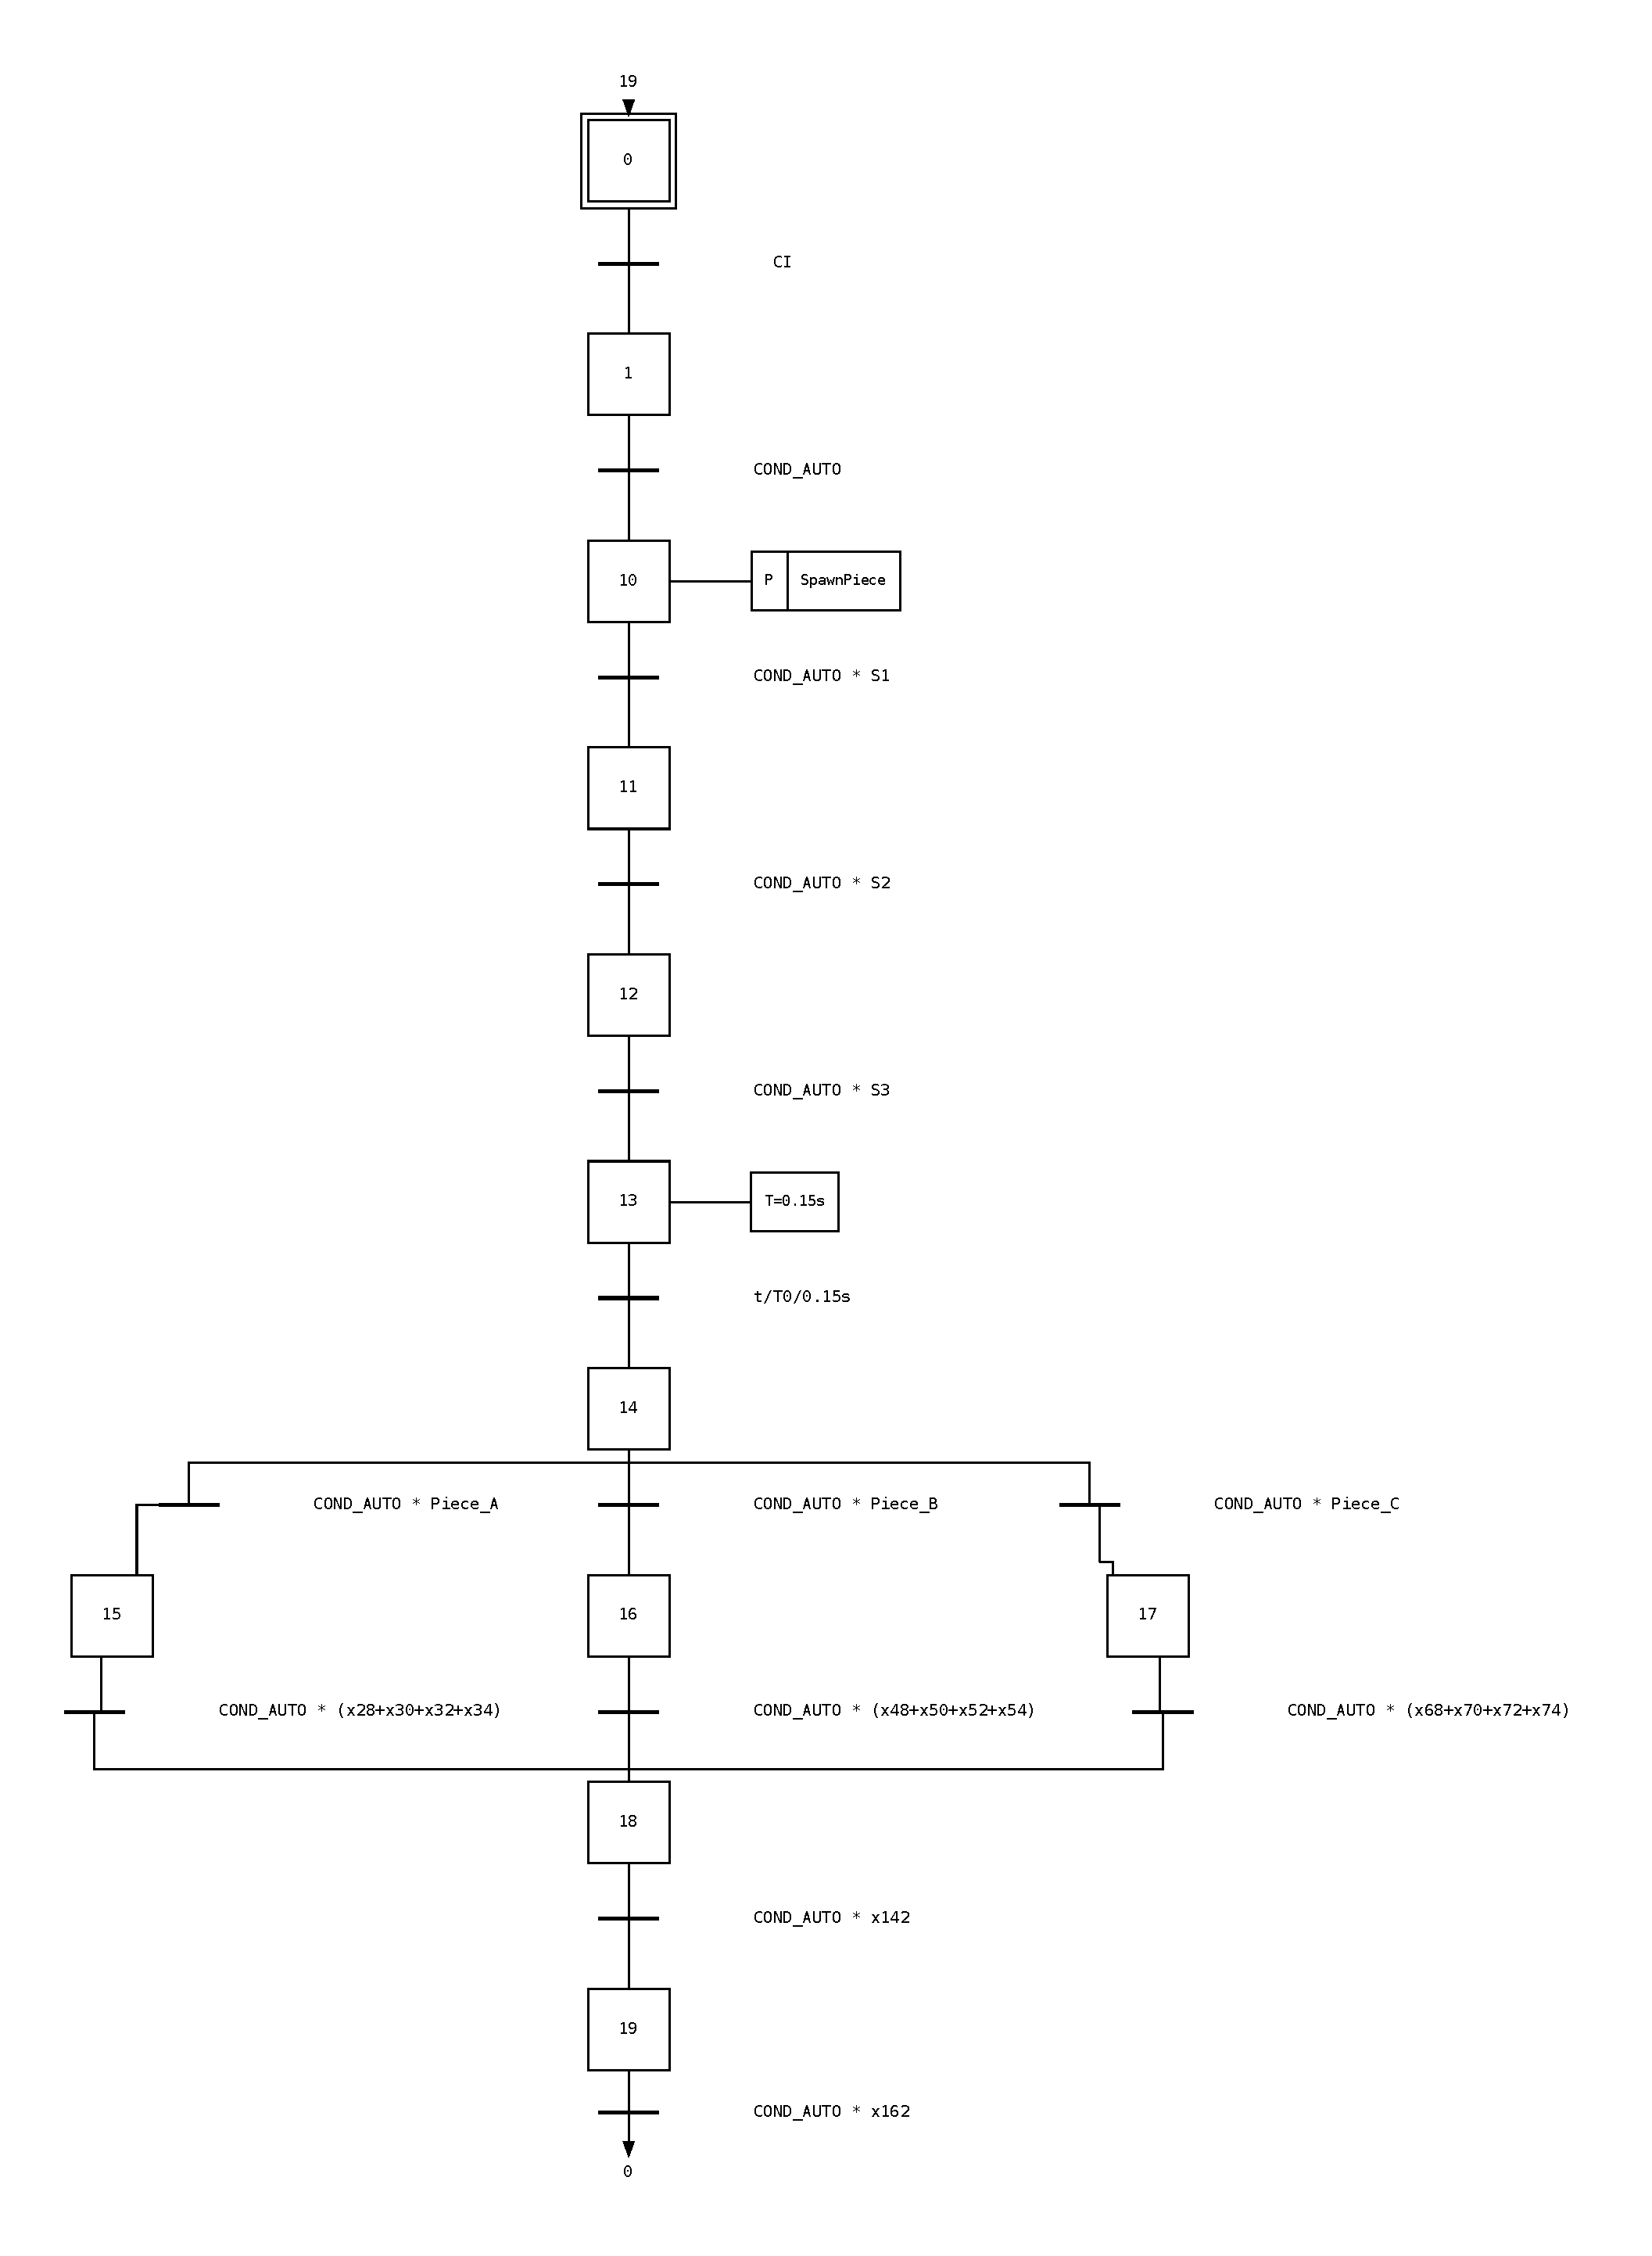
\includegraphics[width=0.85\textwidth]{PDF_GRAFCET/G0.pdf}
\caption{GRAFCET general del sistema}
\label{fig:annex_g0}
\end{figure}

\subsubsection*{\textbf{C.2} GRAFCET de classificació - Estanteria A (G20)}
\addcontentsline{toc}{subsubsection}{\textbf{C.2} GRAFCET de classificació - Estanteria A (G20)}
\label{sec:grafcets_g20}

\begin{figure}[H]
\centering
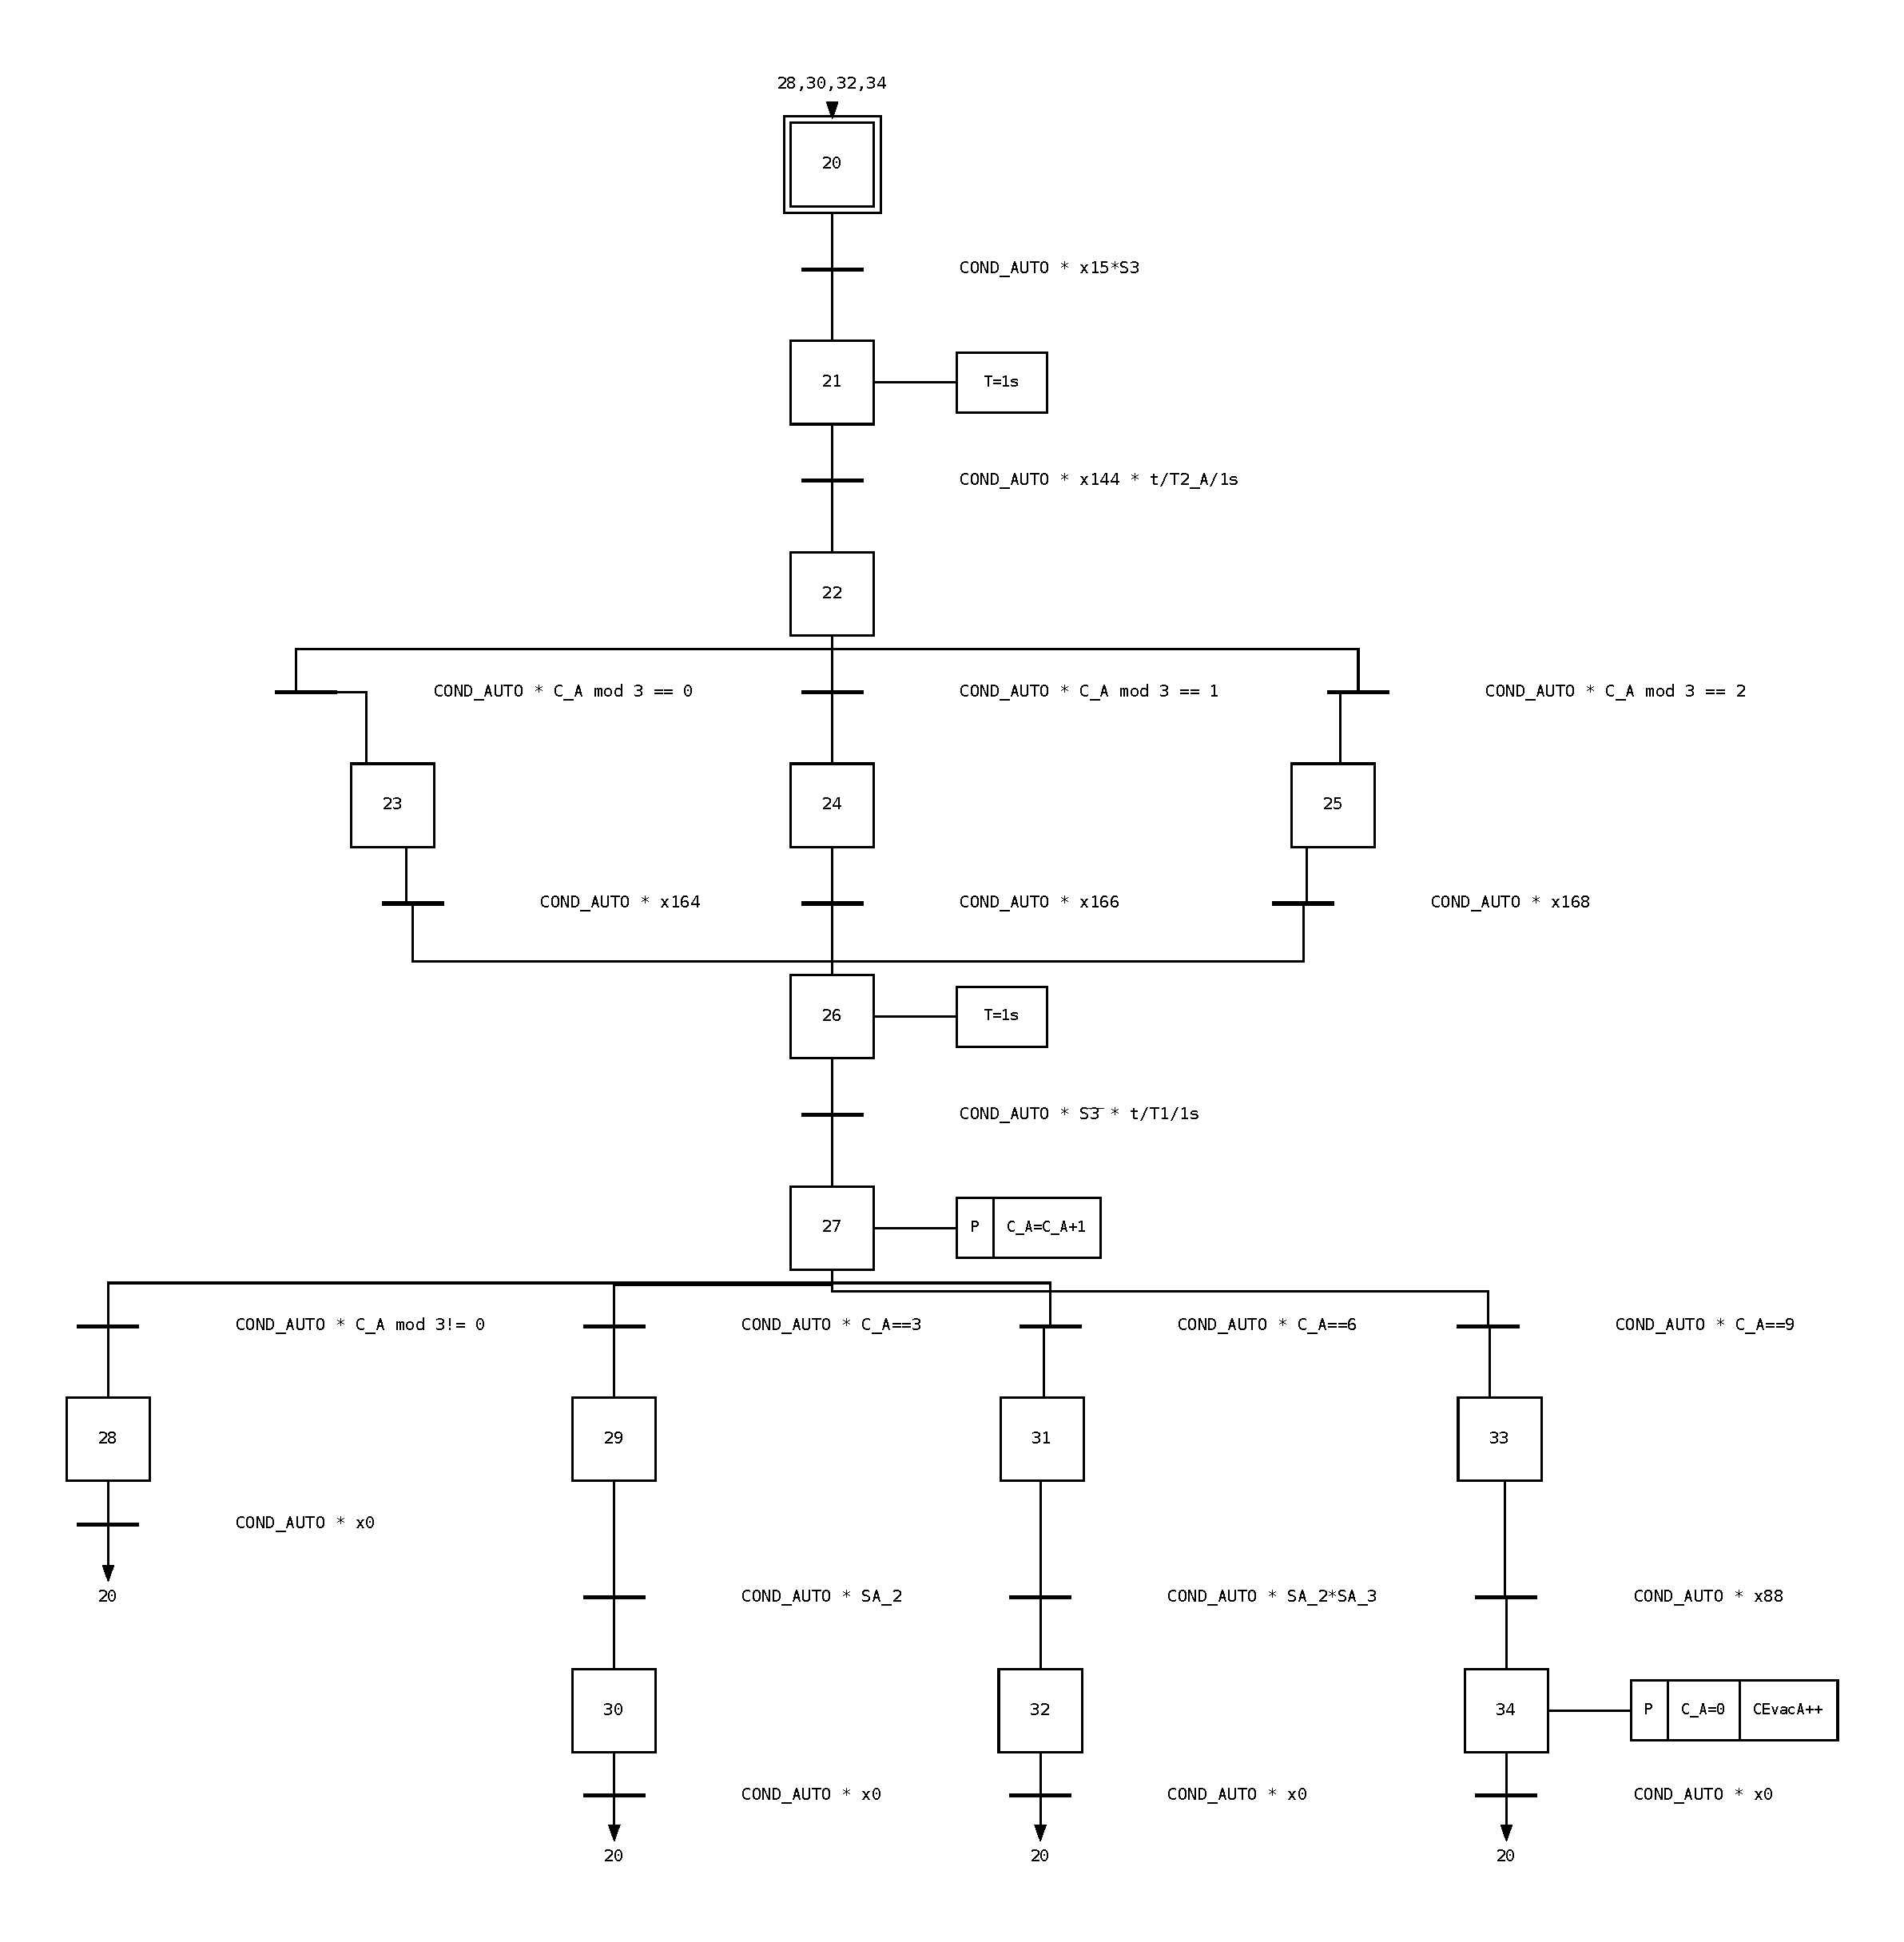
\includegraphics[width=0.85\textwidth]{PDF_GRAFCET/G20.pdf}
\caption{GRAFCET de classificació - Estanteria A}
\label{fig:annex_g20}
\end{figure}

\subsubsection*{\textbf{C.3} GRAFCET d'evacuació}
\addcontentsline{toc}{subsubsection}{\textbf{C.3} GRAFCET d'evacuació}
\label{sec:grafcets_g80}

\begin{figure}[H]
\centering
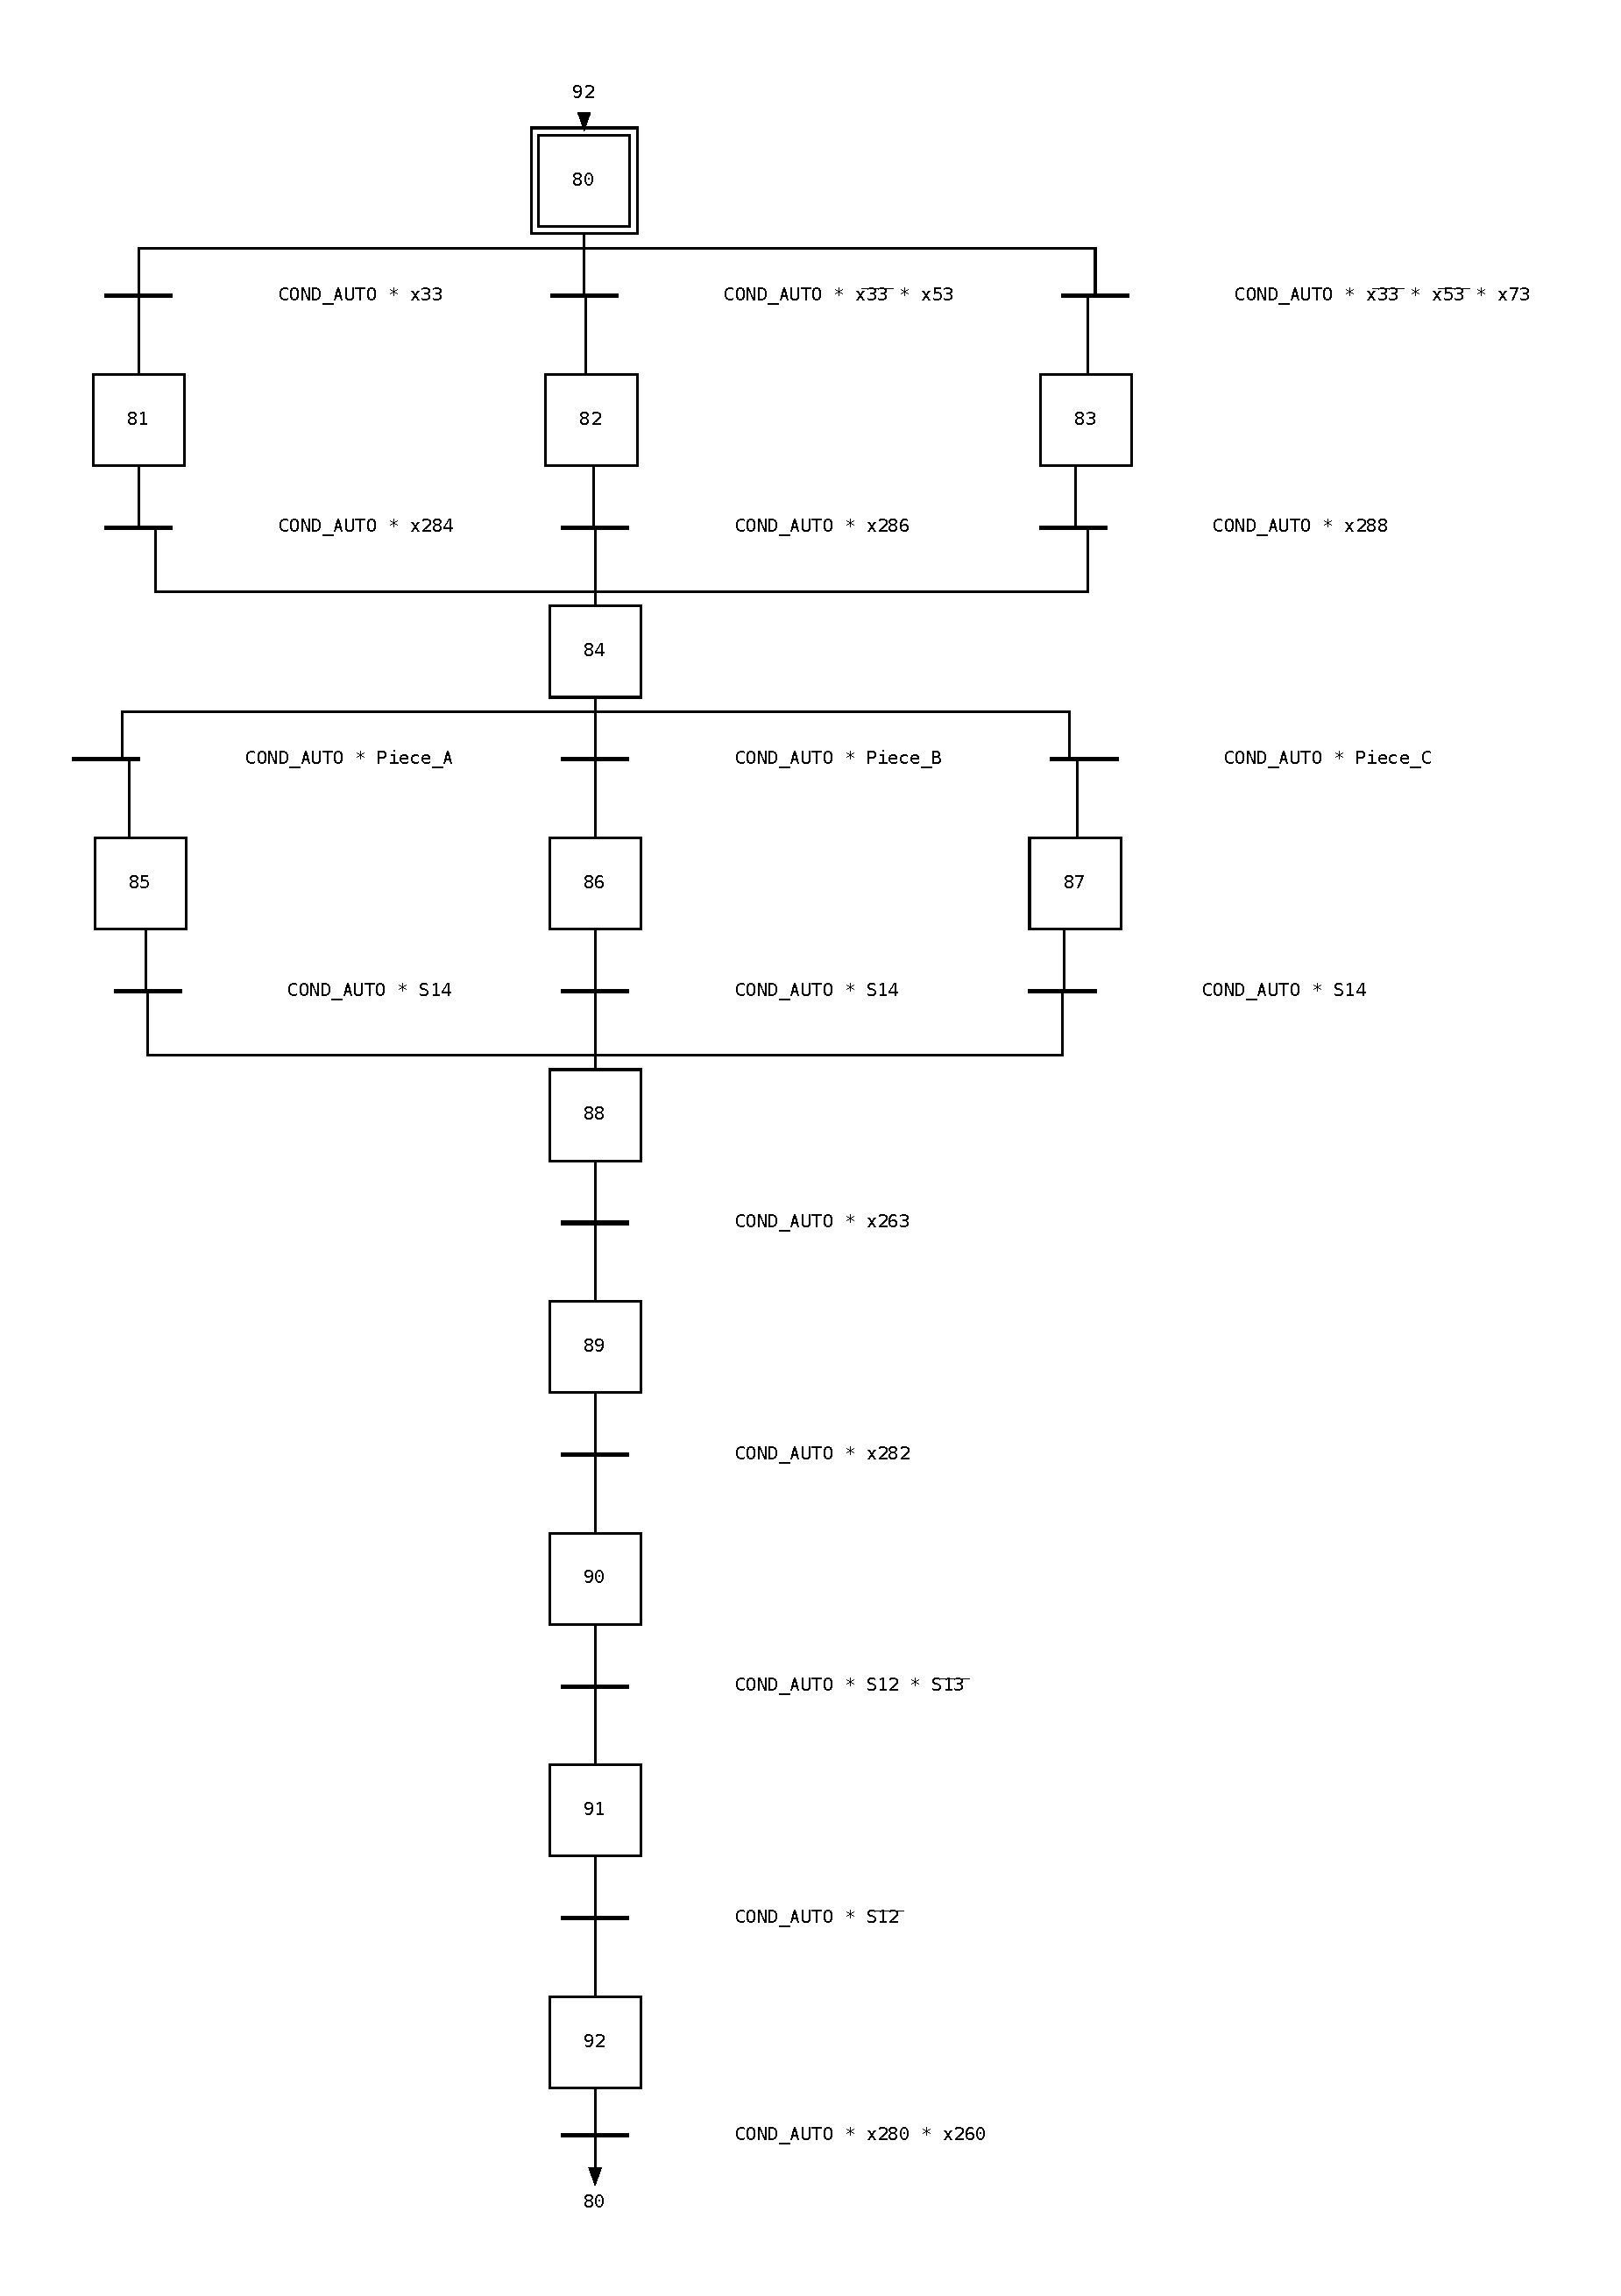
\includegraphics[width=0.85\textwidth]{PDF_GRAFCET/G80.pdf}
\caption{GRAFCET d'evacuació del sistema}
\label{fig:annex_g80}
\end{figure}

\subsubsection*{\textbf{C.4} GRAFCETs de cintes transportadores i rodets de plataforma}
\addcontentsline{toc}{subsubsection}{\textbf{C.4} GRAFCETs de cintes transportadores i rodets de plataforma}
\label{sec:grafcets_g100}
\begin{figure}[H]
\centering
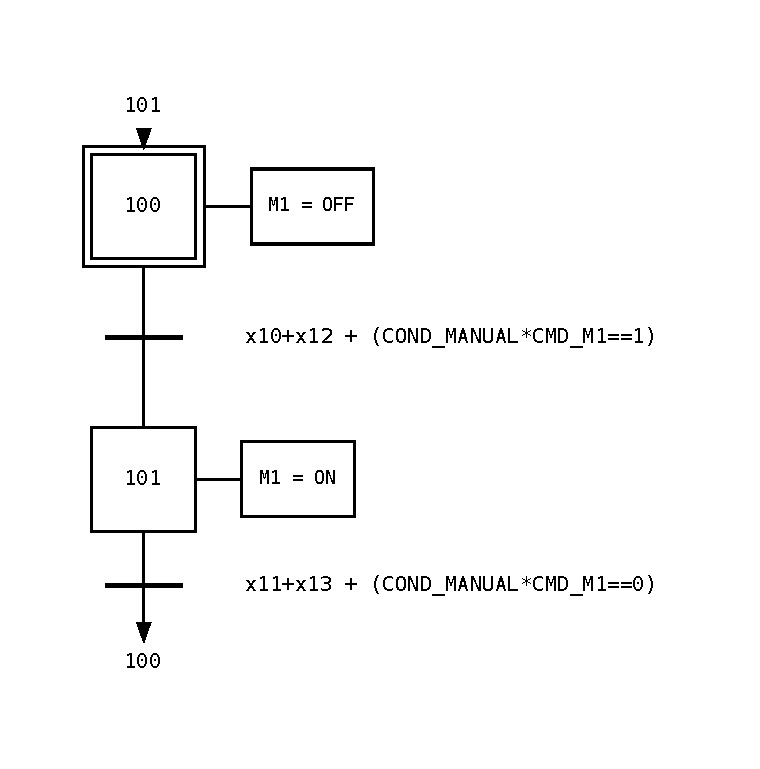
\includegraphics[width=0.75\textwidth]{PDF_GRAFCET/G100.pdf}
\caption{GRAFCET de control de la cinta transportadora}
\label{fig:annex_g100}
\end{figure}

\begin{figure}[H]
\centering
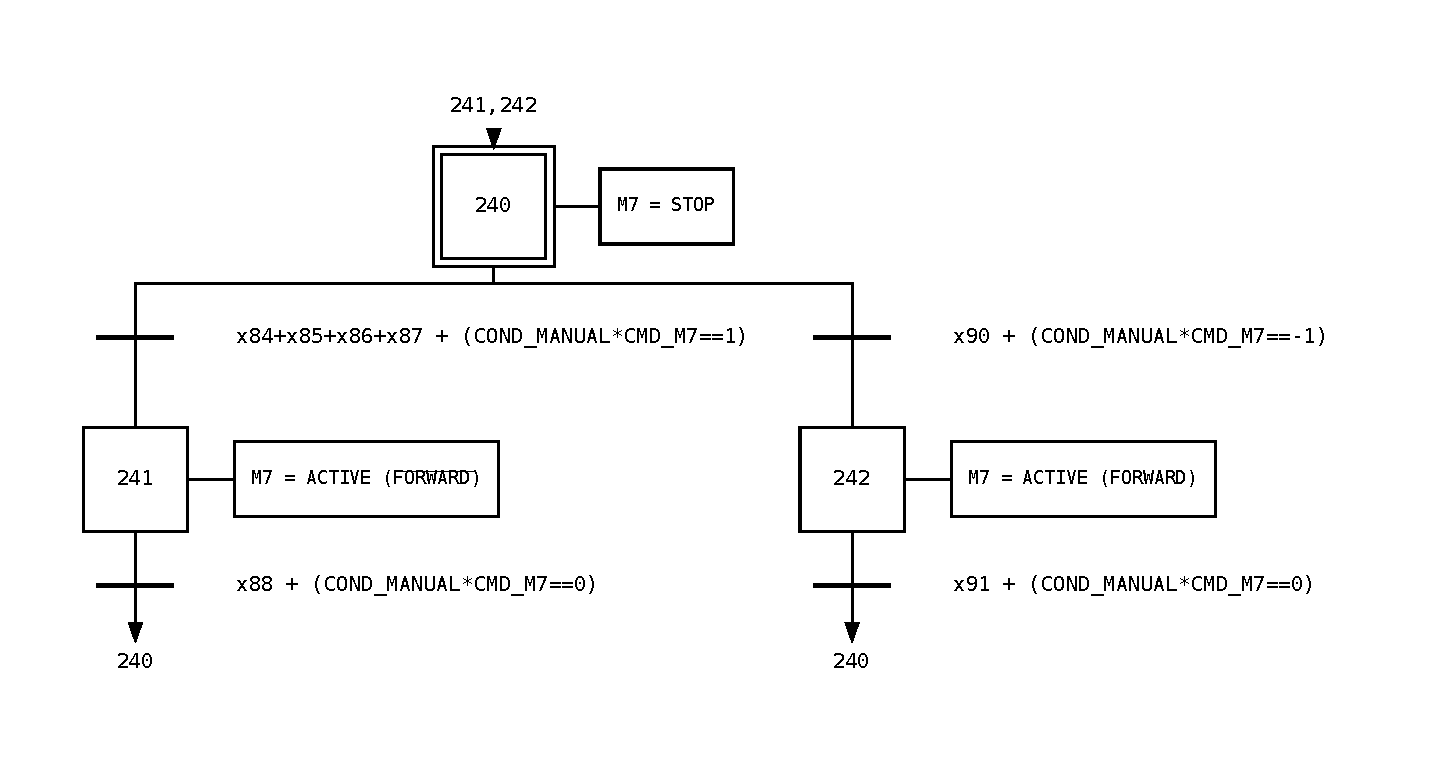
\includegraphics[width=0.75\textwidth]{PDF_GRAFCET/G240.pdf}
\caption{GRAFCET de control dels rodets de plataforma}
\label{fig:annex_g240}
\end{figure}

\subsubsection*{\textbf{C.5} GRAFCET dels transelevadors}
\addcontentsline{toc}{subsubsection}{\textbf{C.5} GRAFCET dels transelevadors}
\label{sec:grafcets_g140}


\begin{figure}[H]
\centering
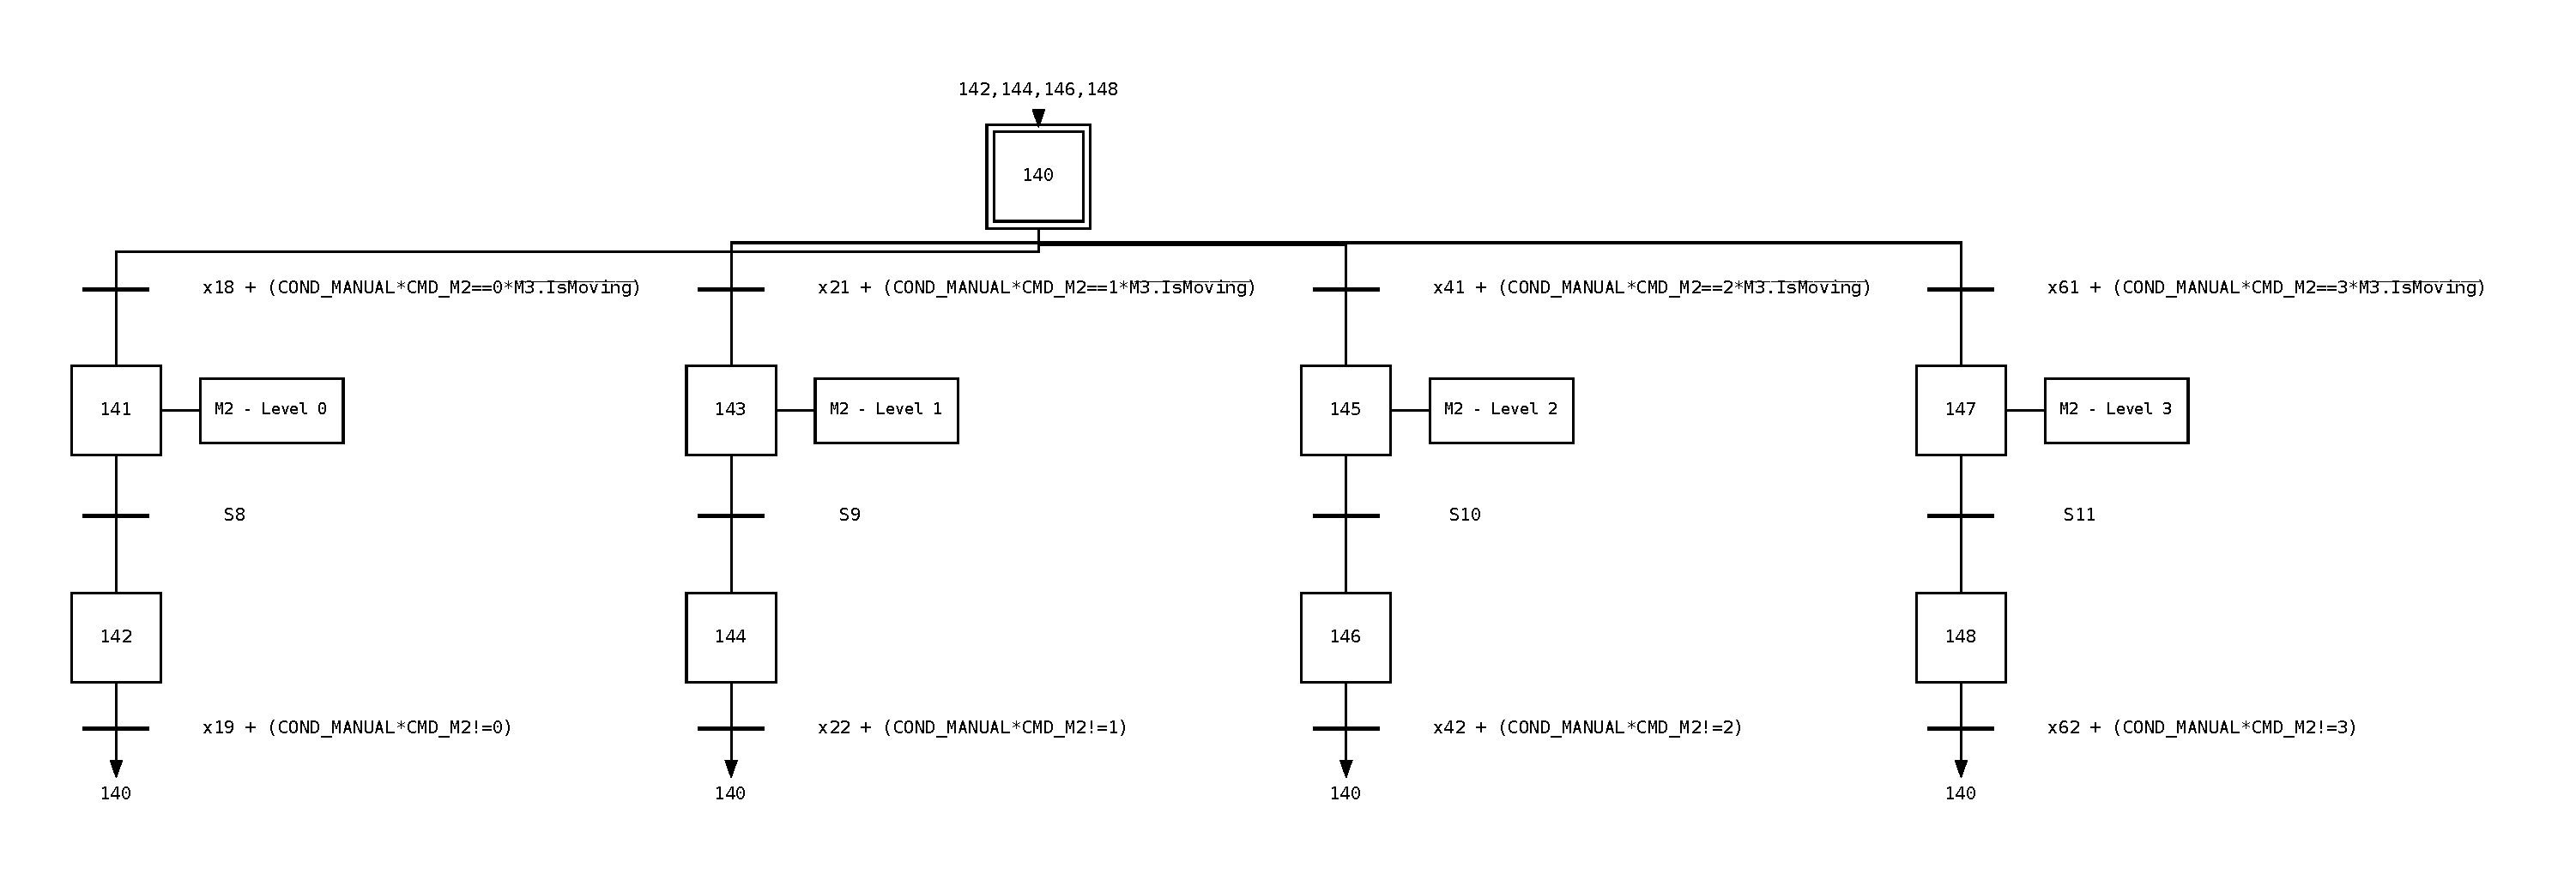
\includegraphics[width=1.1\textwidth]{PDF_GRAFCET/G140.pdf}
\caption{GRAFCET moviment vertical del transelevador 1}
\label{fig:annex_g140}
\end{figure}

\begin{figure}[H]
\centering
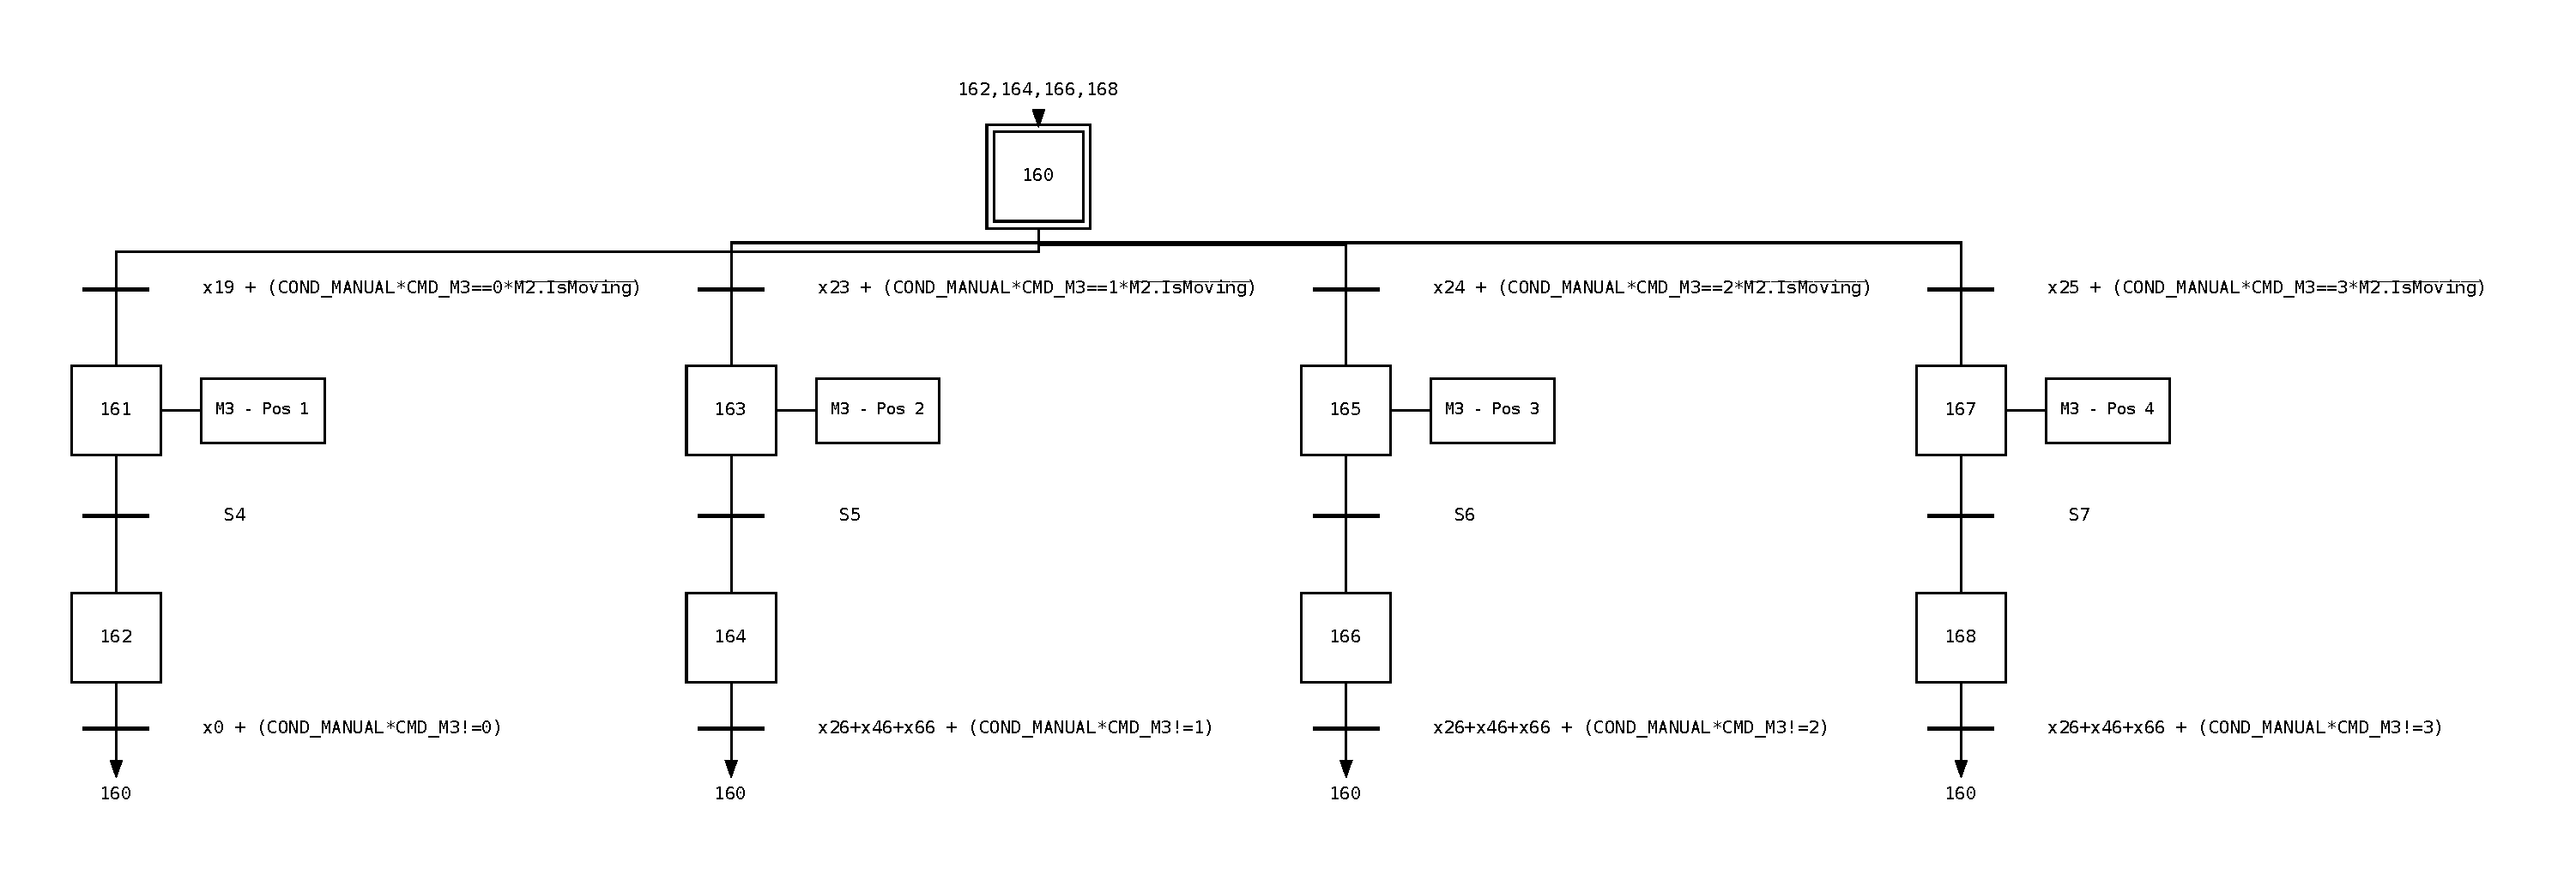
\includegraphics[width=1.1\textwidth]{PDF_GRAFCET/G160.pdf}
\caption{GRAFCET moviment horitzontal del transelevador 1}
\label{fig:annex_g160}
\end{figure}



\subsubsection*{\textbf{C.6} GRAFCET de control i seguretat}
\addcontentsline{toc}{subsubsection}{\textbf{C.6} GRAFCET de control i seguretat}
\label{sec:grafcets_g500}

\begin{figure}[H]
\centering
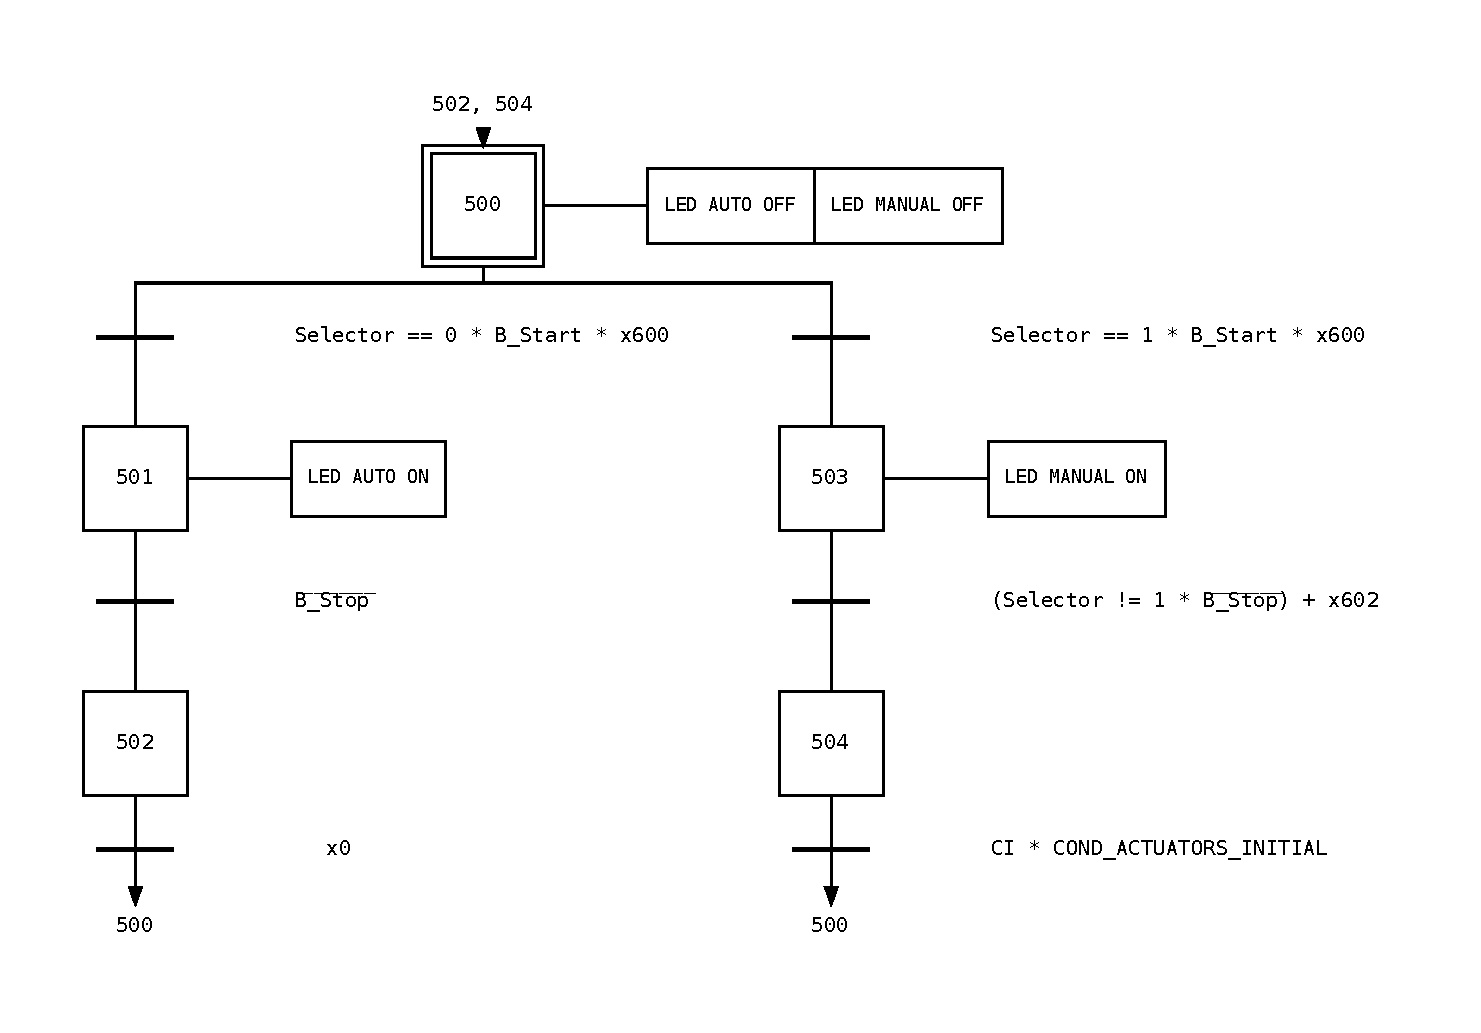
\includegraphics[width=0.8\textwidth]{PDF_GRAFCET/G500.pdf}
\caption{GRAFCET del selector de mode de funcionament}
\label{fig:annex_g500}
\end{figure}


\begin{figure}[H]
\centering
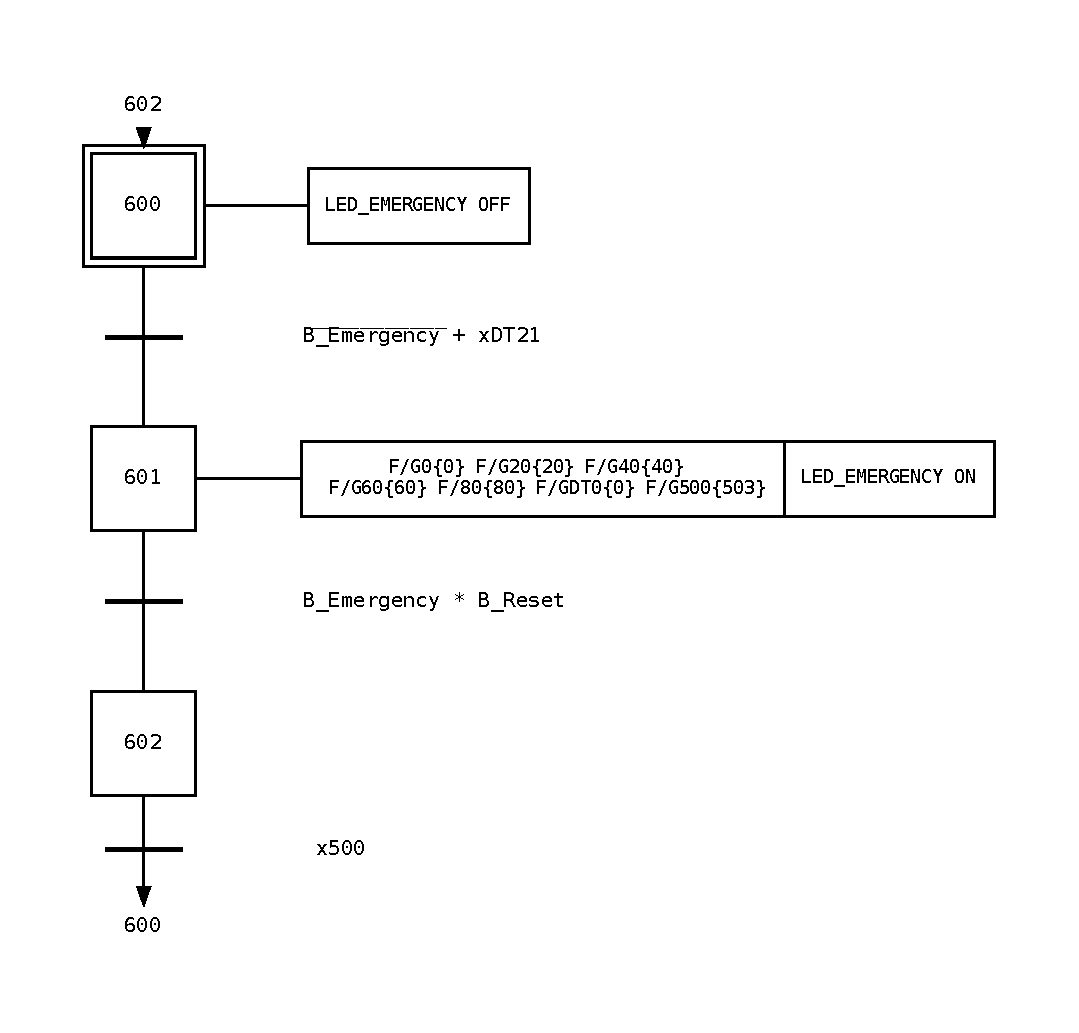
\includegraphics[width=0.6\textwidth]{PDF_GRAFCET/G600.pdf}
\caption{GRAFCET del sistema d'emergència}
\label{fig:annex_g600}
\end{figure}



\begin{figure}[H]
\centering
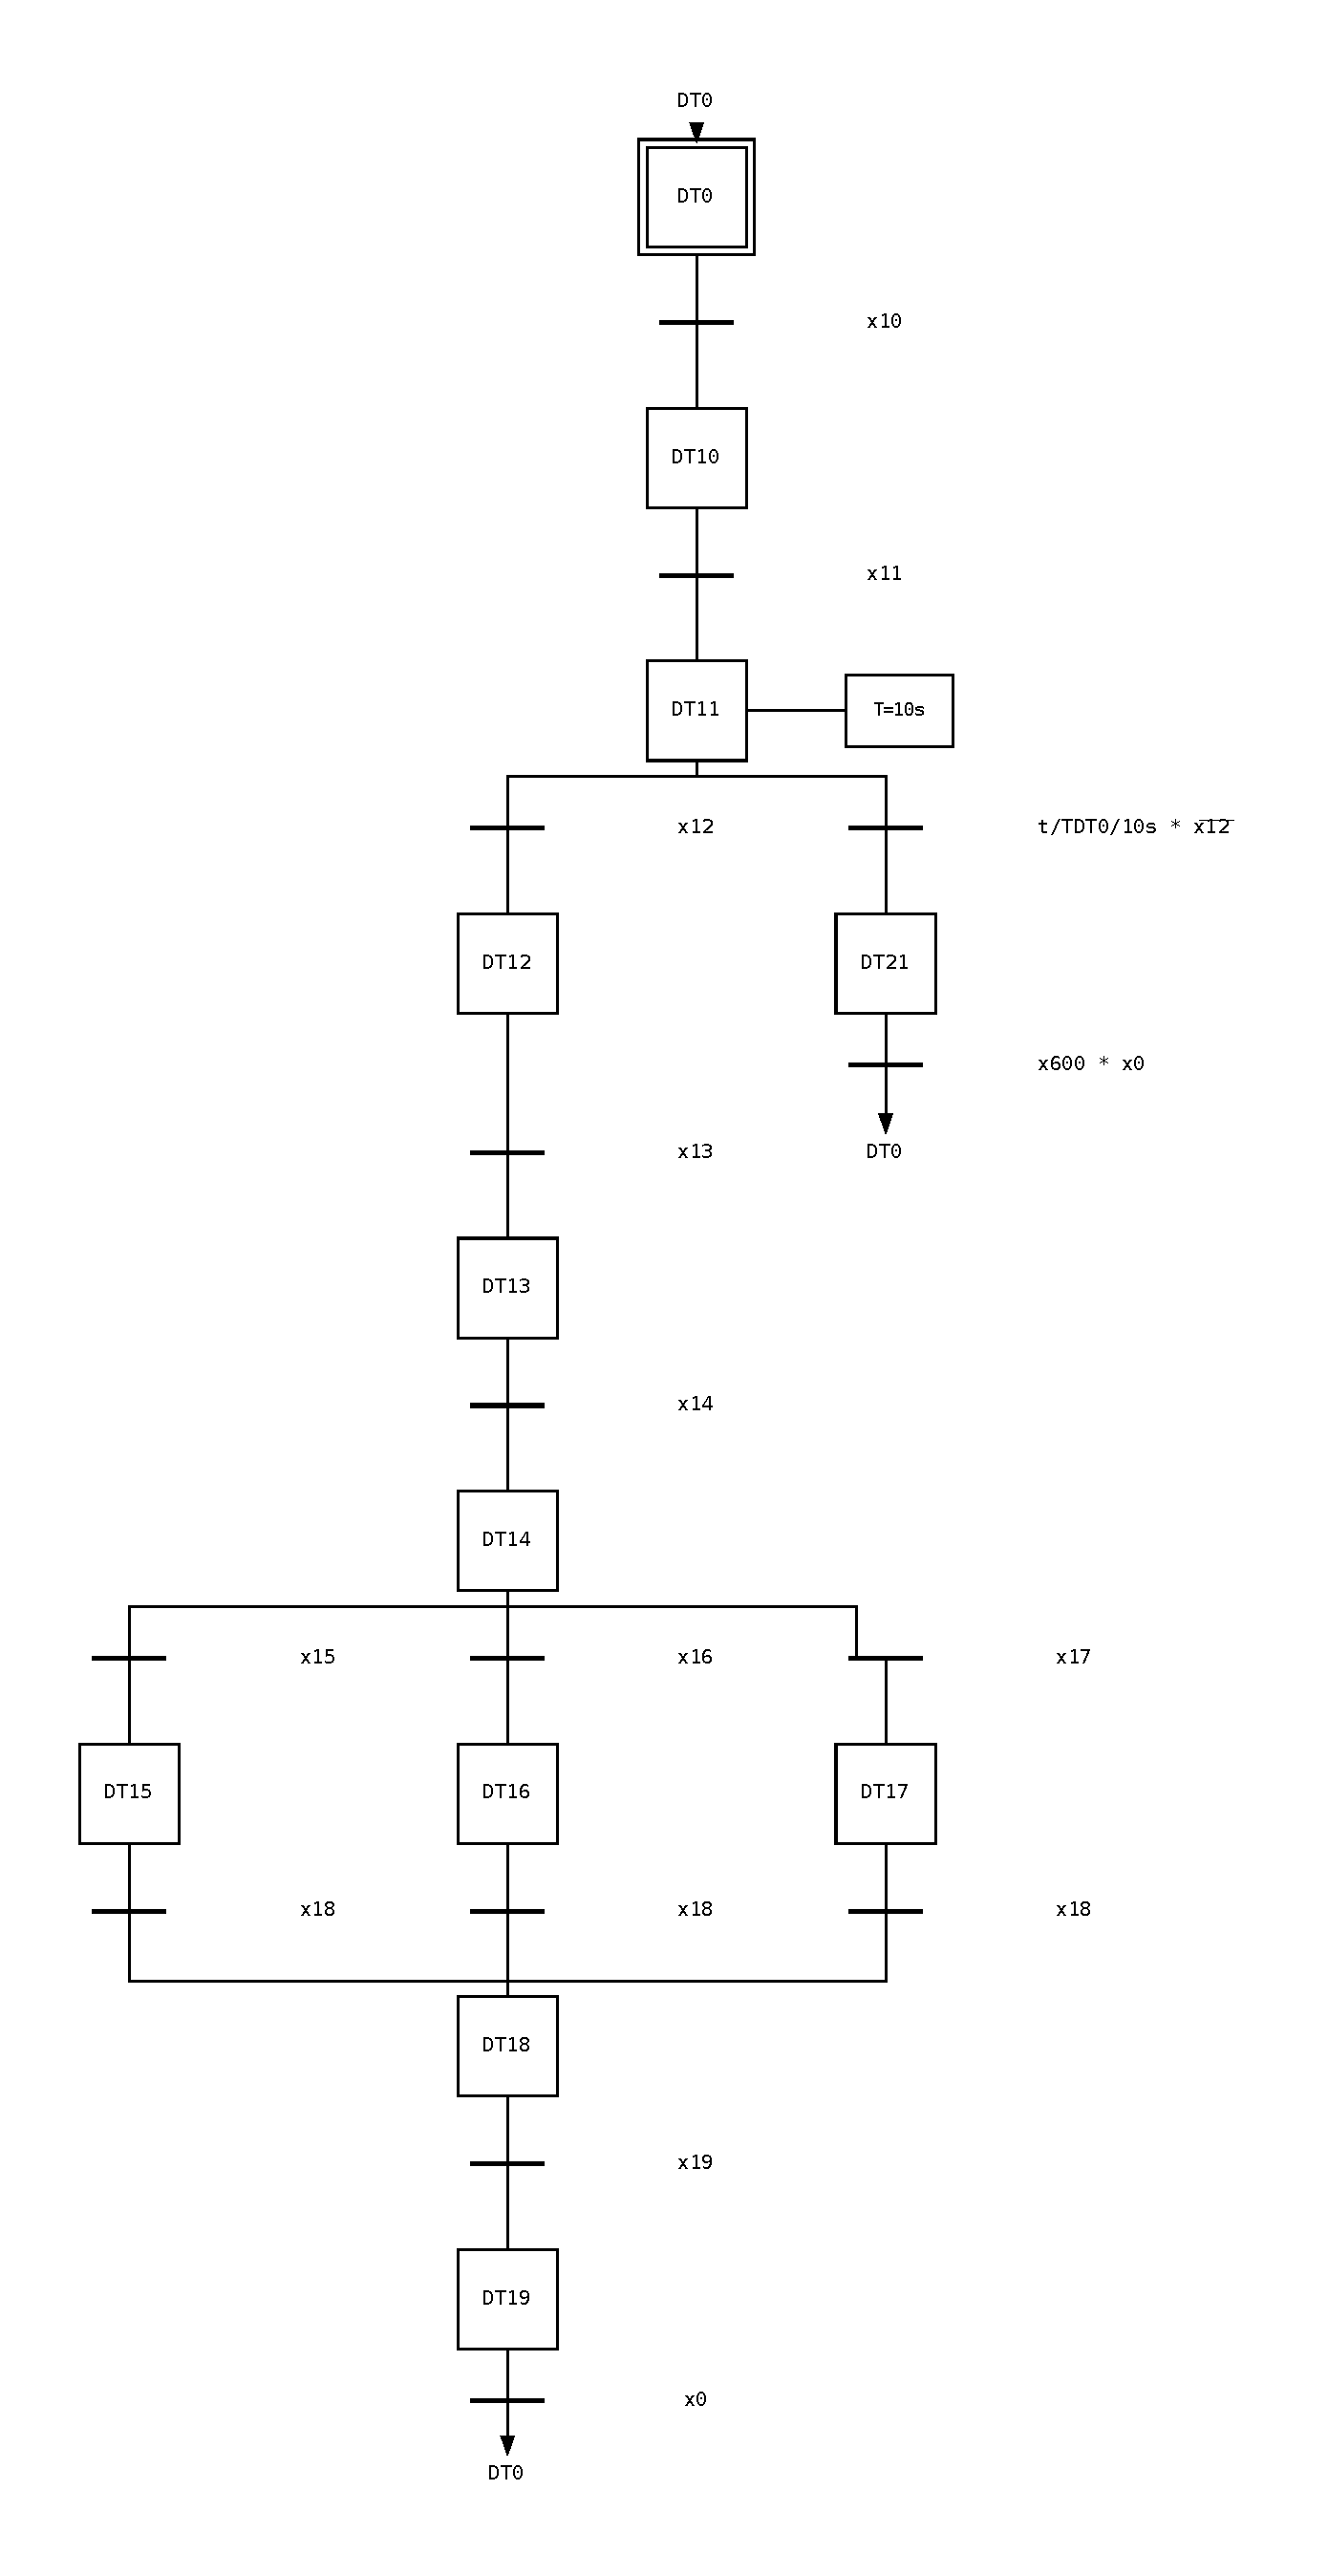
\includegraphics[width=0.75\textwidth]{PDF_GRAFCET/GDT0.pdf}
\caption{GRAFCET de detecció d'avaries (Dual TWEEN)}
\label{fig:annex_gdt0}
\end{figure}

\end{document}
